\chapter{Evaluation}
\label{chap:evaluation}

In this chapter, we evaluate the results of our experiments in the following three sections.
First, we analyze the performance of the \gls{ocr} algorithms for each distortion type.
Then, we compare the performance of the \gls{ocr} algorithms against human judgment.
Finally, we investigate the feasibility of using recognized text \gls{gt} to compare the performance of video codecs.

\section{Performance of Optical Character Recognition}
\label{sec:ocr_performance}

First, we assess the impact of different distortion types on \gls{ocr} performance by comparing the $\overline{\text{CER}}_{\text{c}}$ for various quality levels.
In this section, the $\text{CER}_{\text{c}}$ is calculated in relation to the true \gls{gt} for each image.
We perform this analysis separately for EasyOCR and Tesseract \gls{ocr} compare their performance.
Additionally, we conduct this analysis separately for all nine distortion types.
For the comparison, we plot the $\overline{\text{CER}}_{c}$ with in relation to the \gls{gt} on the y-axis against different quality levels on the x-axis.

\begin{figure}[h!]
\centering
    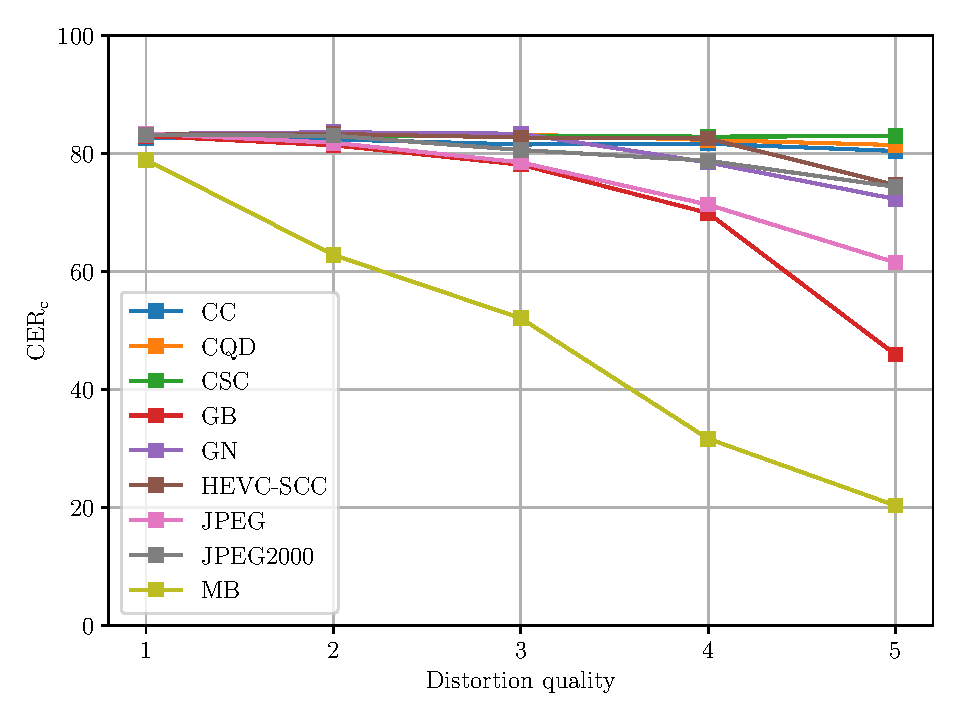
\includegraphics[width=\textwidth]{../../images/analyze/cer_dist_quality_gt_ezocr.pdf}
    \caption{$\overline{\text{CER}}_{\text{c}}$ in relation to the \gls{gt} for different quality levels with EasyOCR.}
\label{fig:cer_dist_quality_gt_ezocr}
\end{figure}

In \autoref{fig:cer_dist_quality_gt_ezocr}, we observe the $\overline{\text{CER}}_{\text{c}}$ in relation to the \gls{gt} for different quality levels using EasyOCR.
We notice a trend that \gls{mb} has the most significant impact on EasyOCR's performance, exhibiting a nearly linear decrease from 80 to 20.
For \gls{jpeg} and \gls{gb} EasyOCR displays similar behavior until quality level 4, after which it experiences a steeper decline for \gls{gb}.
This may be due to the blurring of images greatly affecting the legibility of text, with letters becoming indistinct and merging together.
For \gls{gn}, \gls{jpeg2000} and \gls{hevcscc} EasyOCR exhibits similar performance, experiencing a slight decline at quality level 5.
The remaining distortions have minimal impact on performance, which we expect since color distortions do not directly affect text shapes.

\begin{figure}[h!]
\centering
    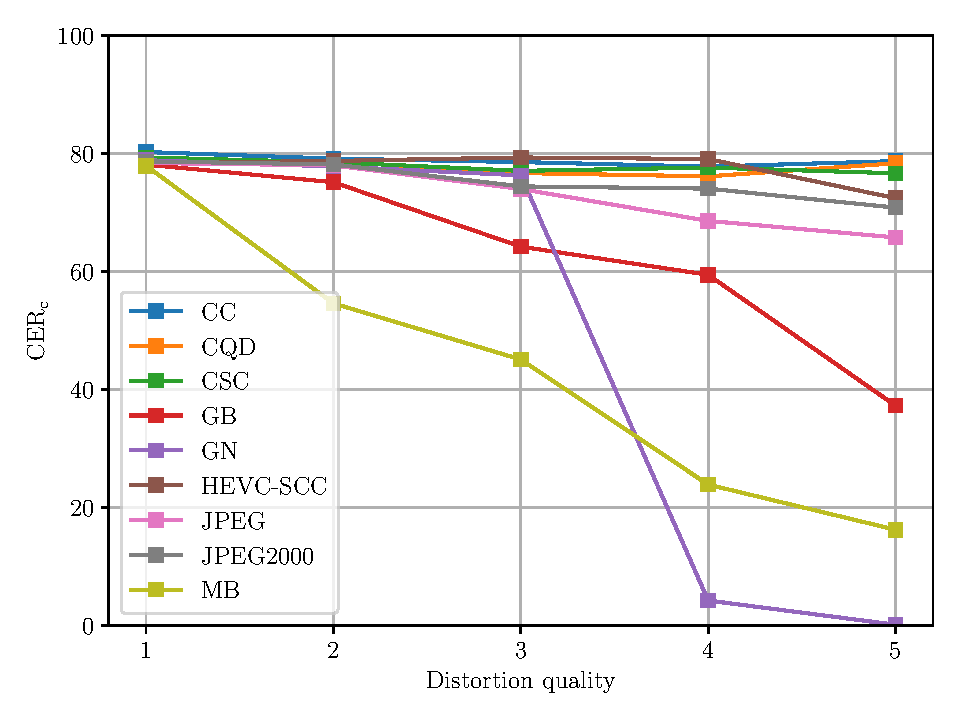
\includegraphics[width=\textwidth]{../../images/analyze/cer_dist_quality_gt_tess.pdf}
    \caption{$\overline{\text{CER}}_{\text{c}}$ in relation to the \gls{gt} for different quality levels with Tesseract \gls{ocr}.}
\label{fig:cer_dist_quality_gt_tesseract}
\end{figure}

In \autoref{fig:cer_dist_quality_gt_tesseract}, we can see the same analysis for Tesseract \gls{ocr}.
We see a steady decrease in $\overline{\text{CER}}_{\text{c}}$ for \gls{mb} and \gls{gb}, with the former exhibiting a steeper decline.
However, the most noteworthy finding is the significant drop in $\overline{\text{CER}}_{\text{c}}$ for \gls{gn} at quality level 4, reaching 0 at quality level 5.
This sudden decline is particularly surprising when compared to other types of distortion.
Among the distortions analyzed, \gls{cc}, \gls{cqd}, and \gls{csc} do not impact the performance.
The results for \gls{cc} even demonstrate a slightly higher $\overline{\text{CER}}_{\text{c}}$ at quality level 5 compared to previous levels.
This phenomenon can possibly be attributed to \gls{cc}'s ability to enhance the distinction between the text and the background, acting almost like an image preprocessing step for the \gls{ocr}.

In summary, our results reveal that \gls{mb} and \gls{gb} have a substantial impact on the performance of both EasyOCR and Tesseract \gls{ocr} algorithms.
Additionally, both \gls{ocr} algorithms demonstrate superior performance across images with \gls{cc}, \gls{cqd}, and \gls{csc}.
However, the most remarkable discovery is the significant drop in the $\overline{\text{CER}}_{\text{c}}$ for Gaussian noise at quality level 4, even reaching 0 at quality level 5, for Tesseract OCR.
This suggests that EasyOCR exhibits greater robustness to \gls{gn} compared to Tesseract \gls{ocr} .
Overall, EasyOCR outperforms Tesseract \gls{ocr}, with the highest $\overline{\text{CER}}_{\text{c}}$ of approximately 83 for EasyOCR, while Tesseract \gls{ocr} only achieves around 80.




\section{Comparison With Human Judgment}
\label{sec:comparison_with_human_judgment}

In this section, we compare the performance of the \gls{ocr} algorithms with human judgment.
We first plot the $\overline{\text{CER}}_{\text{c}}$ on the x-axis against the \gls{mos} on the y-axis for each distortion type.
Furthermore, we separate the plots, one for EasyOCR and one for Tesseract \gls{ocr}.
For each metric, the mean is calculated over all images for each quality level and distortion type.
Additionally, compared to the last section, we calculate the $\text{CER}_{\text{c}}$ in relation to the text predictions on the reference image instead of the \gls{gt}.
Since the \gls{mos} is created by humans comparing the distorted images to the reference images, it makes it a fairer comparison.

% mos vs cer mean in relation to reference for easyocr
\begin{figure}[h!]
\centering
    \begin{subfigure}[b]{0.32\textwidth}
        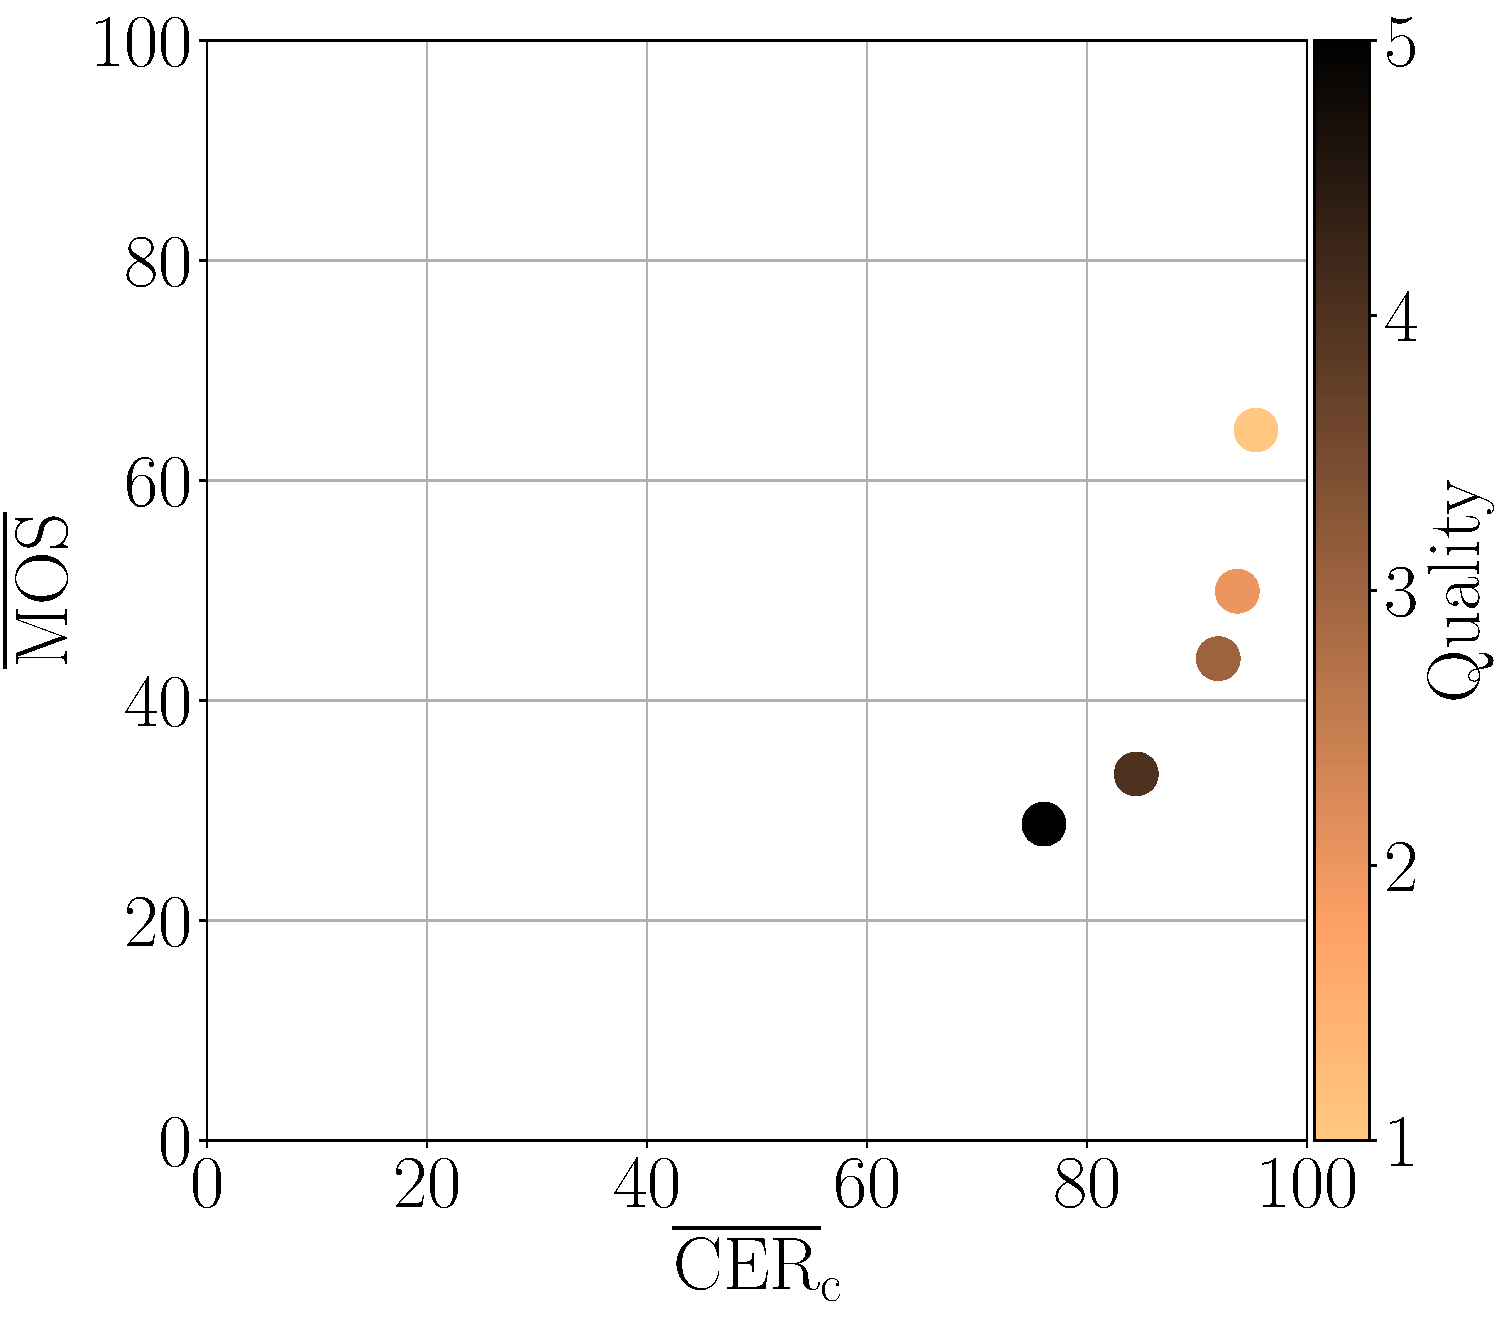
\includegraphics[width=\textwidth]{../../images/analyze/mos_cer_ref_mean_ezocr_GN.pdf}
        \caption{GN}
        \label{fig:mos_cer_ref_mean_ezocr_GN}
    \end{subfigure}%
    \hfill
    \begin{subfigure}[b]{0.32\textwidth}
        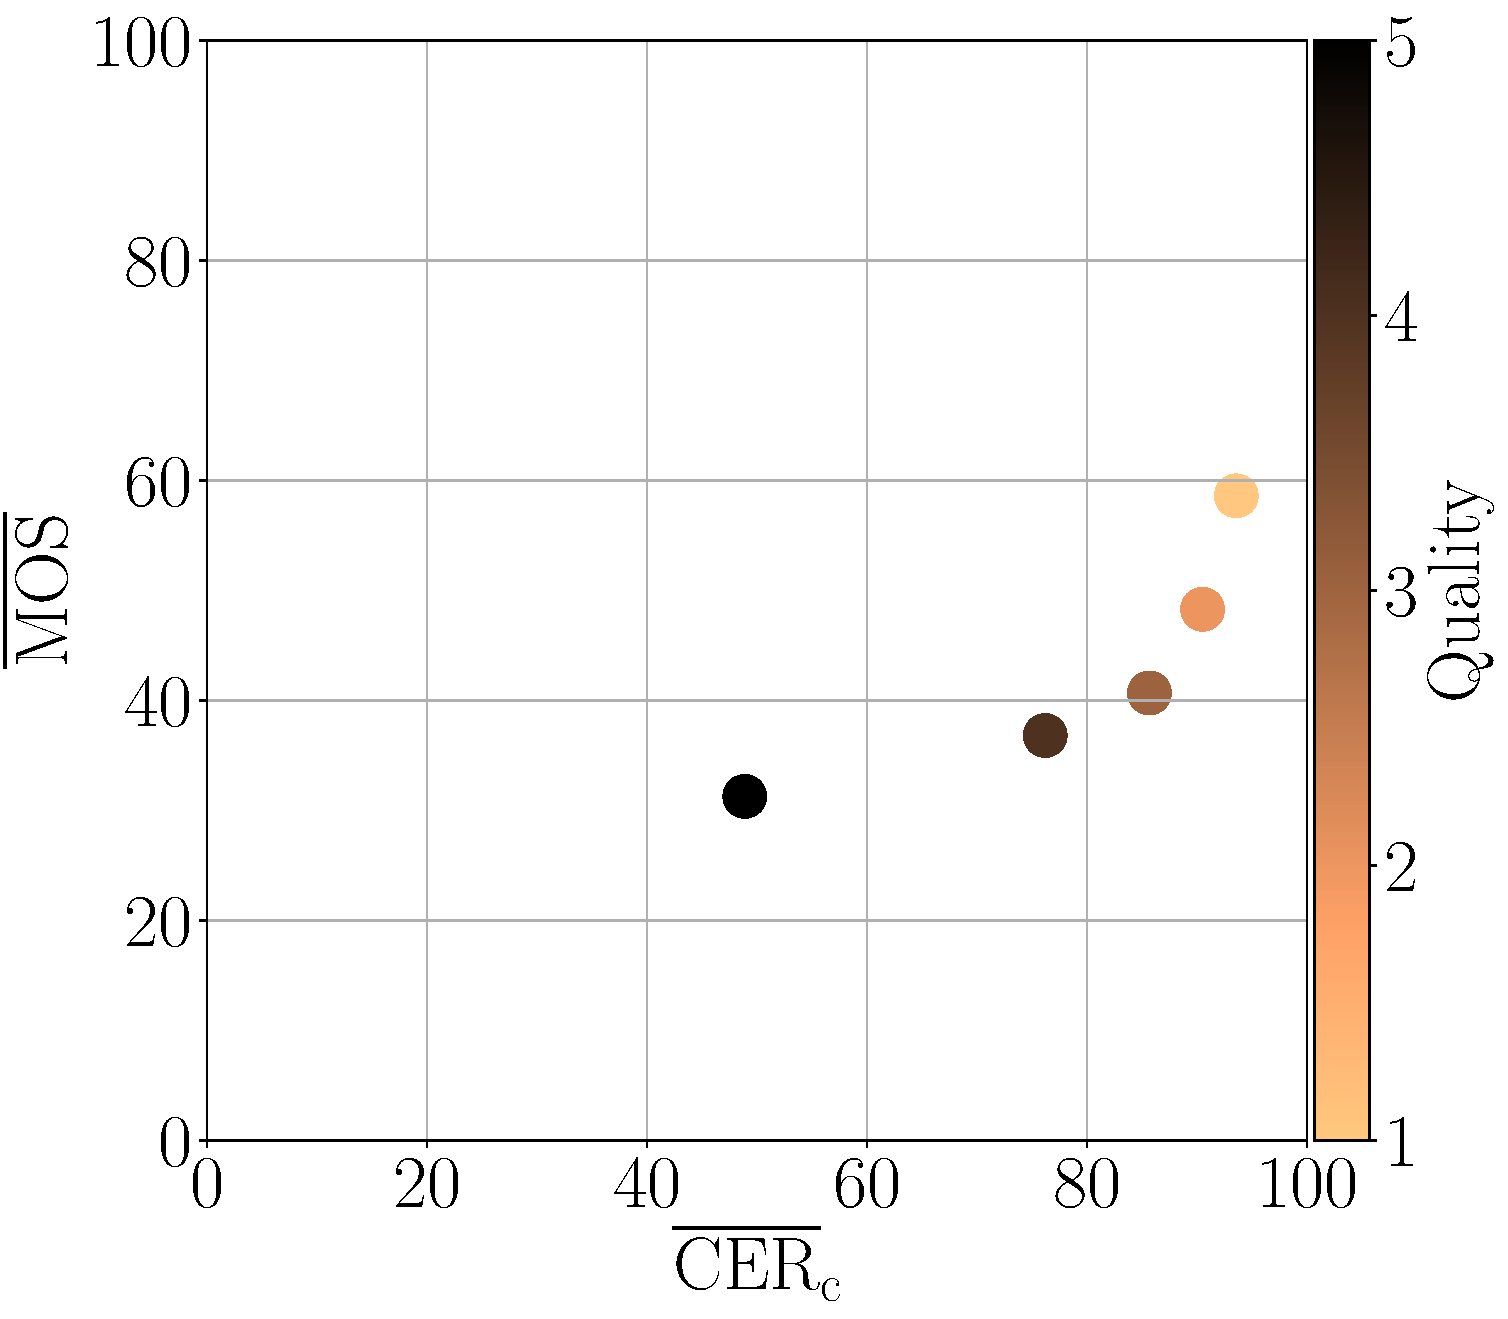
\includegraphics[width=\textwidth]{../../images/analyze/mos_cer_ref_mean_ezocr_GB.pdf}
        \caption{GB}
        \label{fig:mos_cer_ref_mean_ezocr_GB}
    \end{subfigure}%
    \hfill
    \begin{subfigure}[b]{0.32\textwidth}
        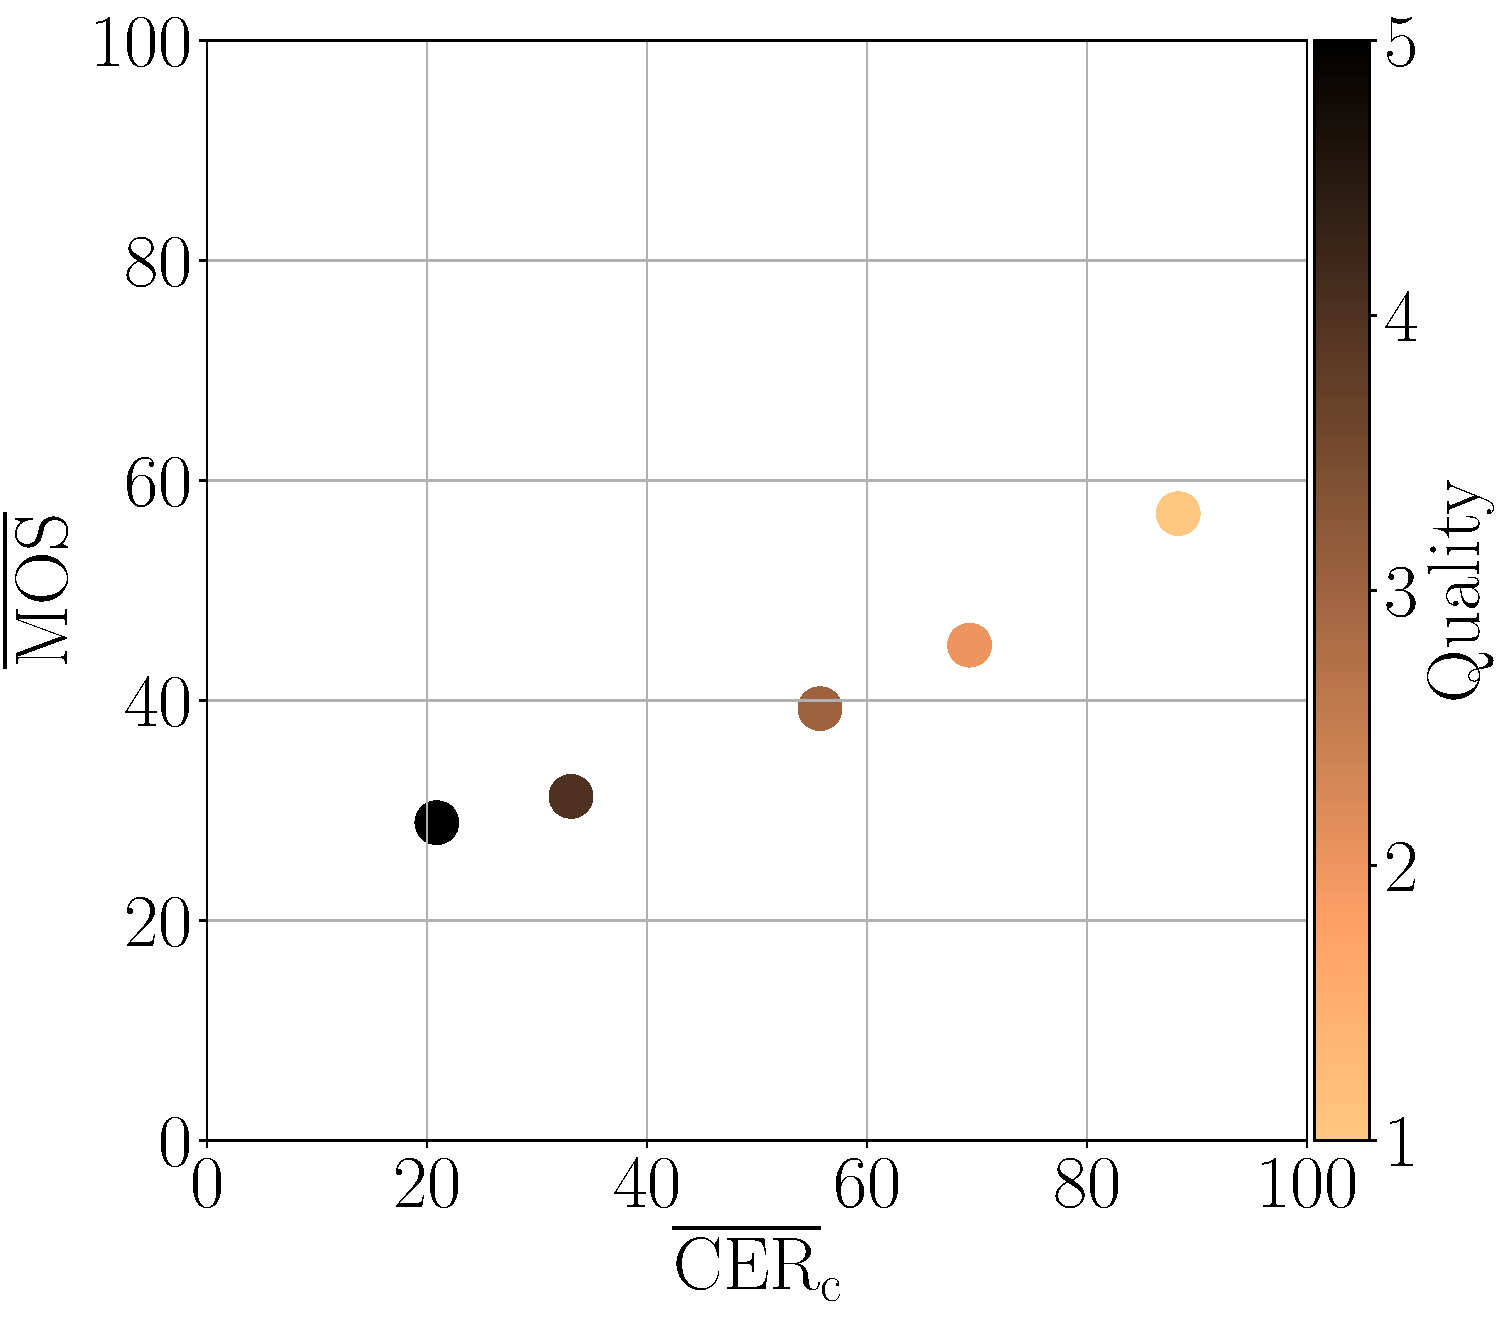
\includegraphics[width=\textwidth]{../../images/analyze/mos_cer_ref_mean_ezocr_MB.pdf}
        \caption{MB}
        \label{fig:mos_cer_ref_mean_ezocr_MB}
    \end{subfigure}%
    \newline
    \begin{subfigure}[b]{0.32\textwidth}
        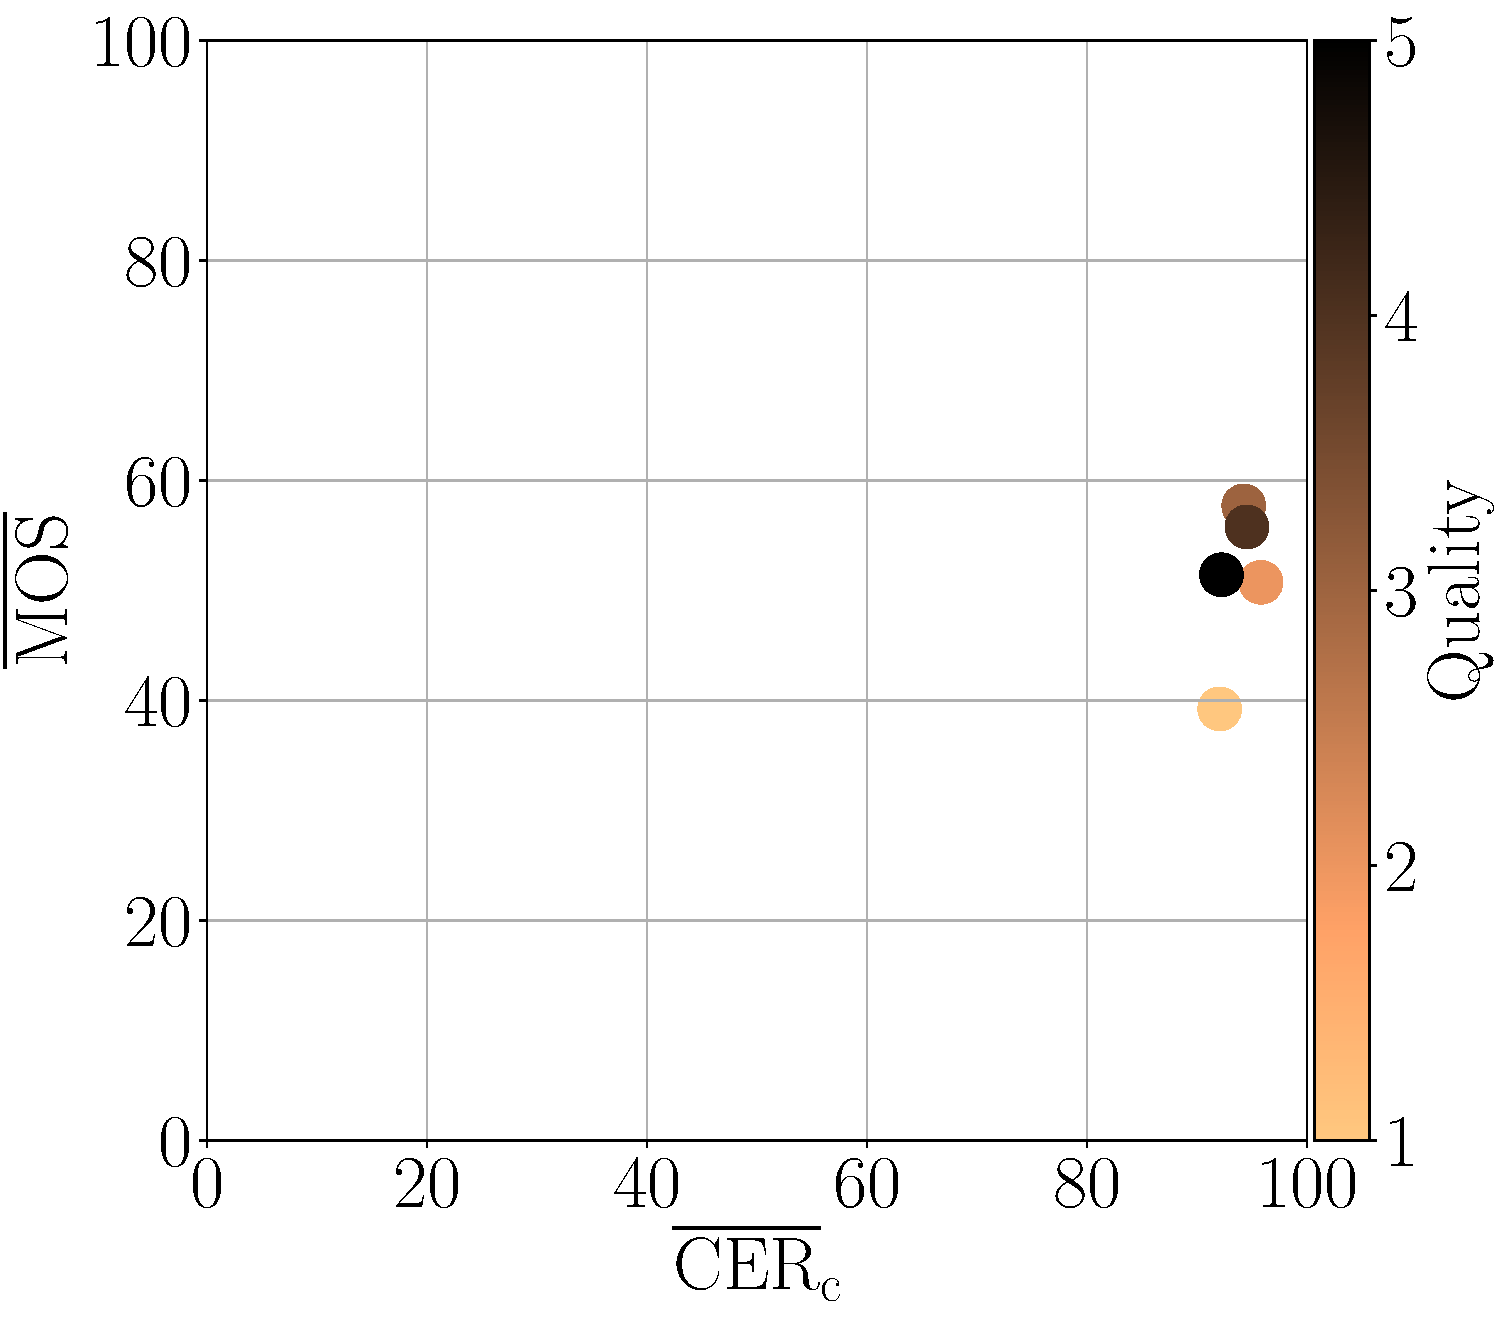
\includegraphics[width=\textwidth]{../../images/analyze/mos_cer_ref_mean_ezocr_CC.pdf}
        \caption{CC}
        \label{fig:mos_cer_ref_mean_ezocr_CC}
    \end{subfigure}%
    \hfill
    \begin{subfigure}[b]{0.32\textwidth}
        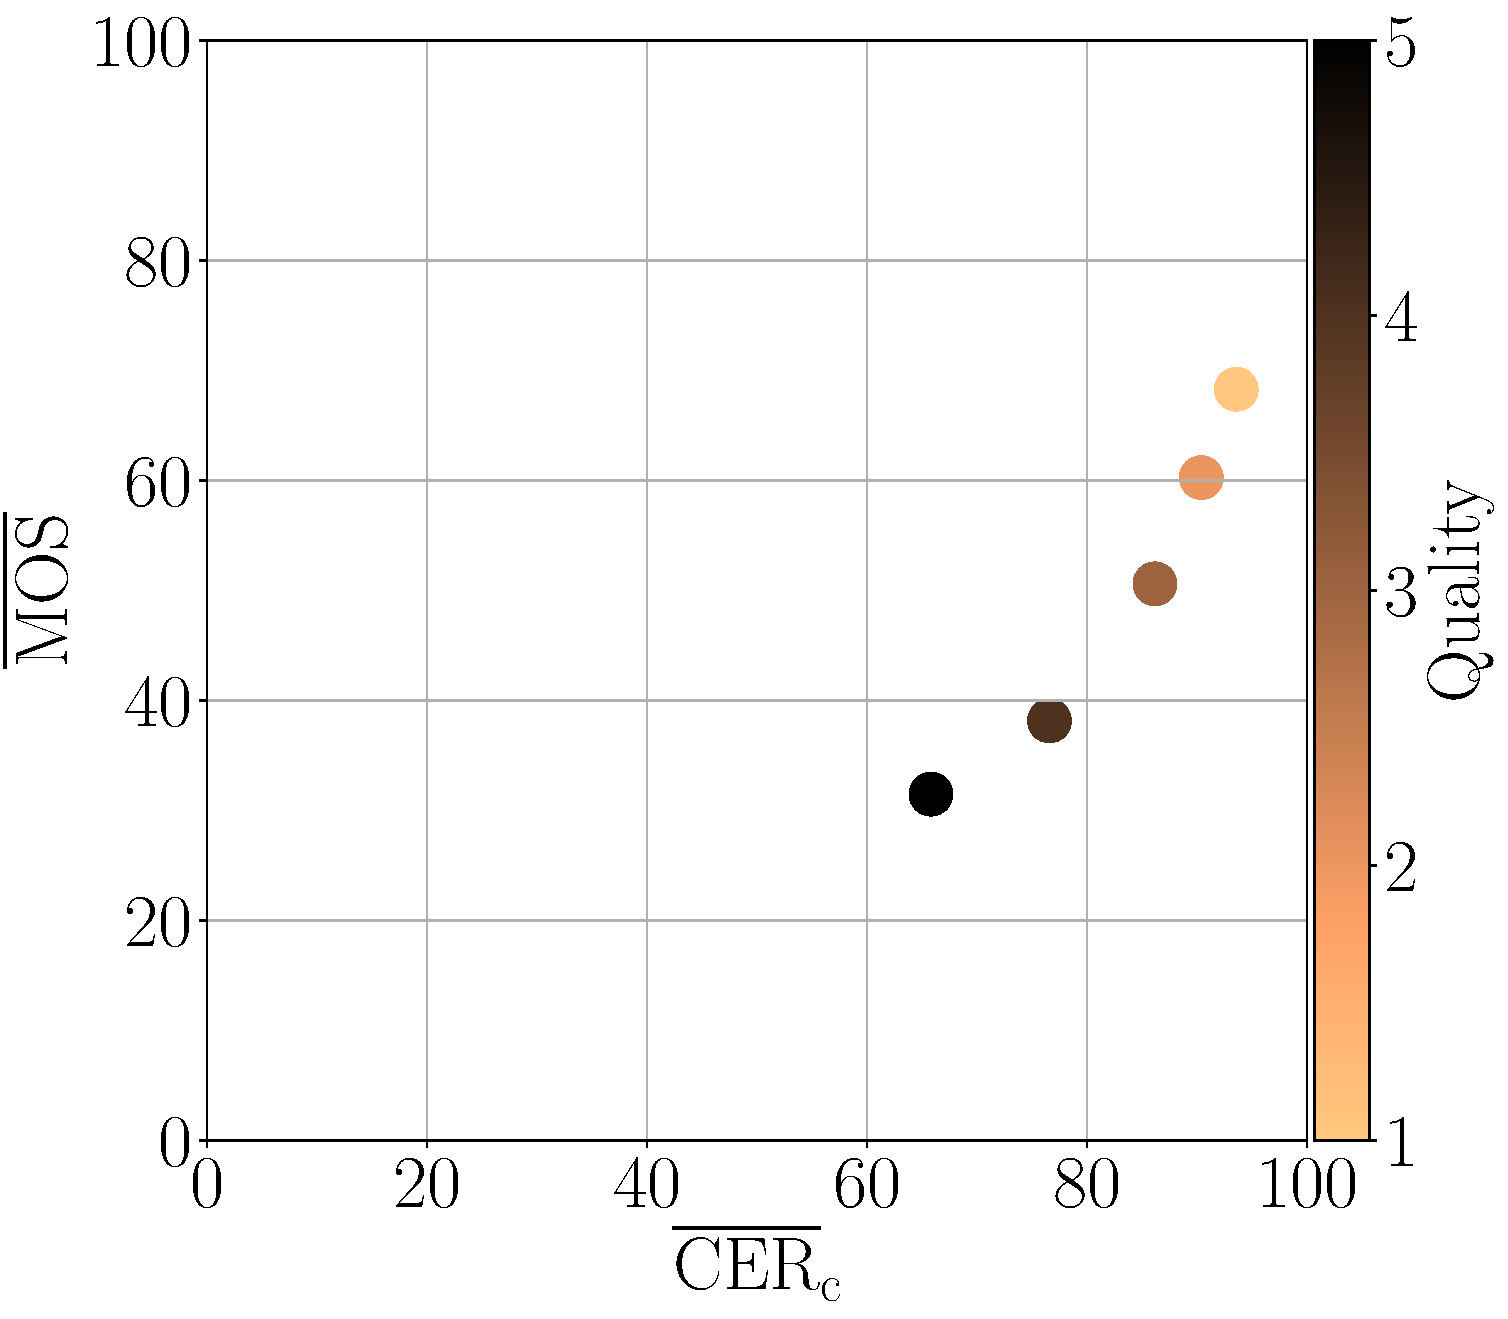
\includegraphics[width=\textwidth]{../../images/analyze/mos_cer_ref_mean_ezocr_JPEG.pdf}
        \caption{JPEG}
        \label{fig:mos_cer_ref_mean_ezocr_JPEG}
    \end{subfigure}%
    \hfill
    \begin{subfigure}[b]{0.32\textwidth}
        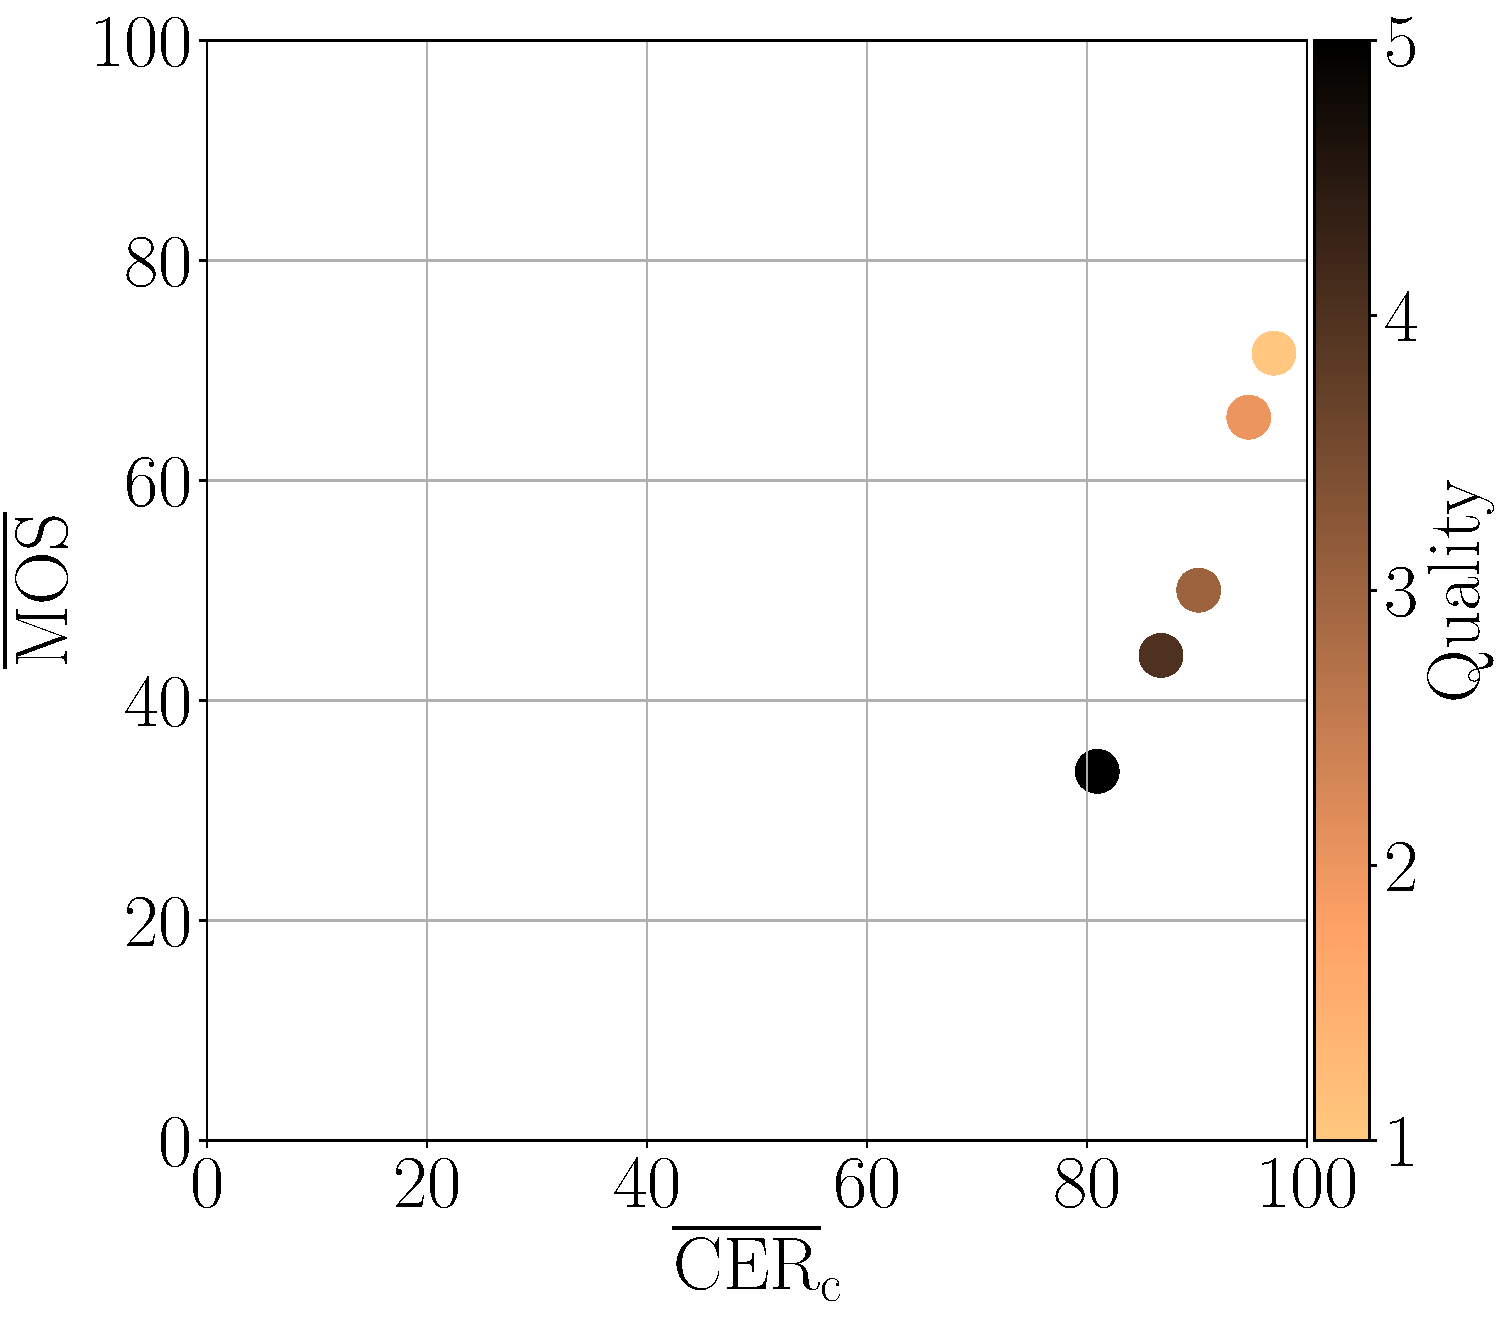
\includegraphics[width=\textwidth]{../../images/analyze/mos_cer_ref_mean_ezocr_JPEG2000.pdf}
        \caption{JPEG2000}
        \label{fig:mos_cer_ref_mean_ezocr_JPEG2000}
    \end{subfigure}%
    \newline
    \begin{subfigure}[b]{0.32\textwidth}
        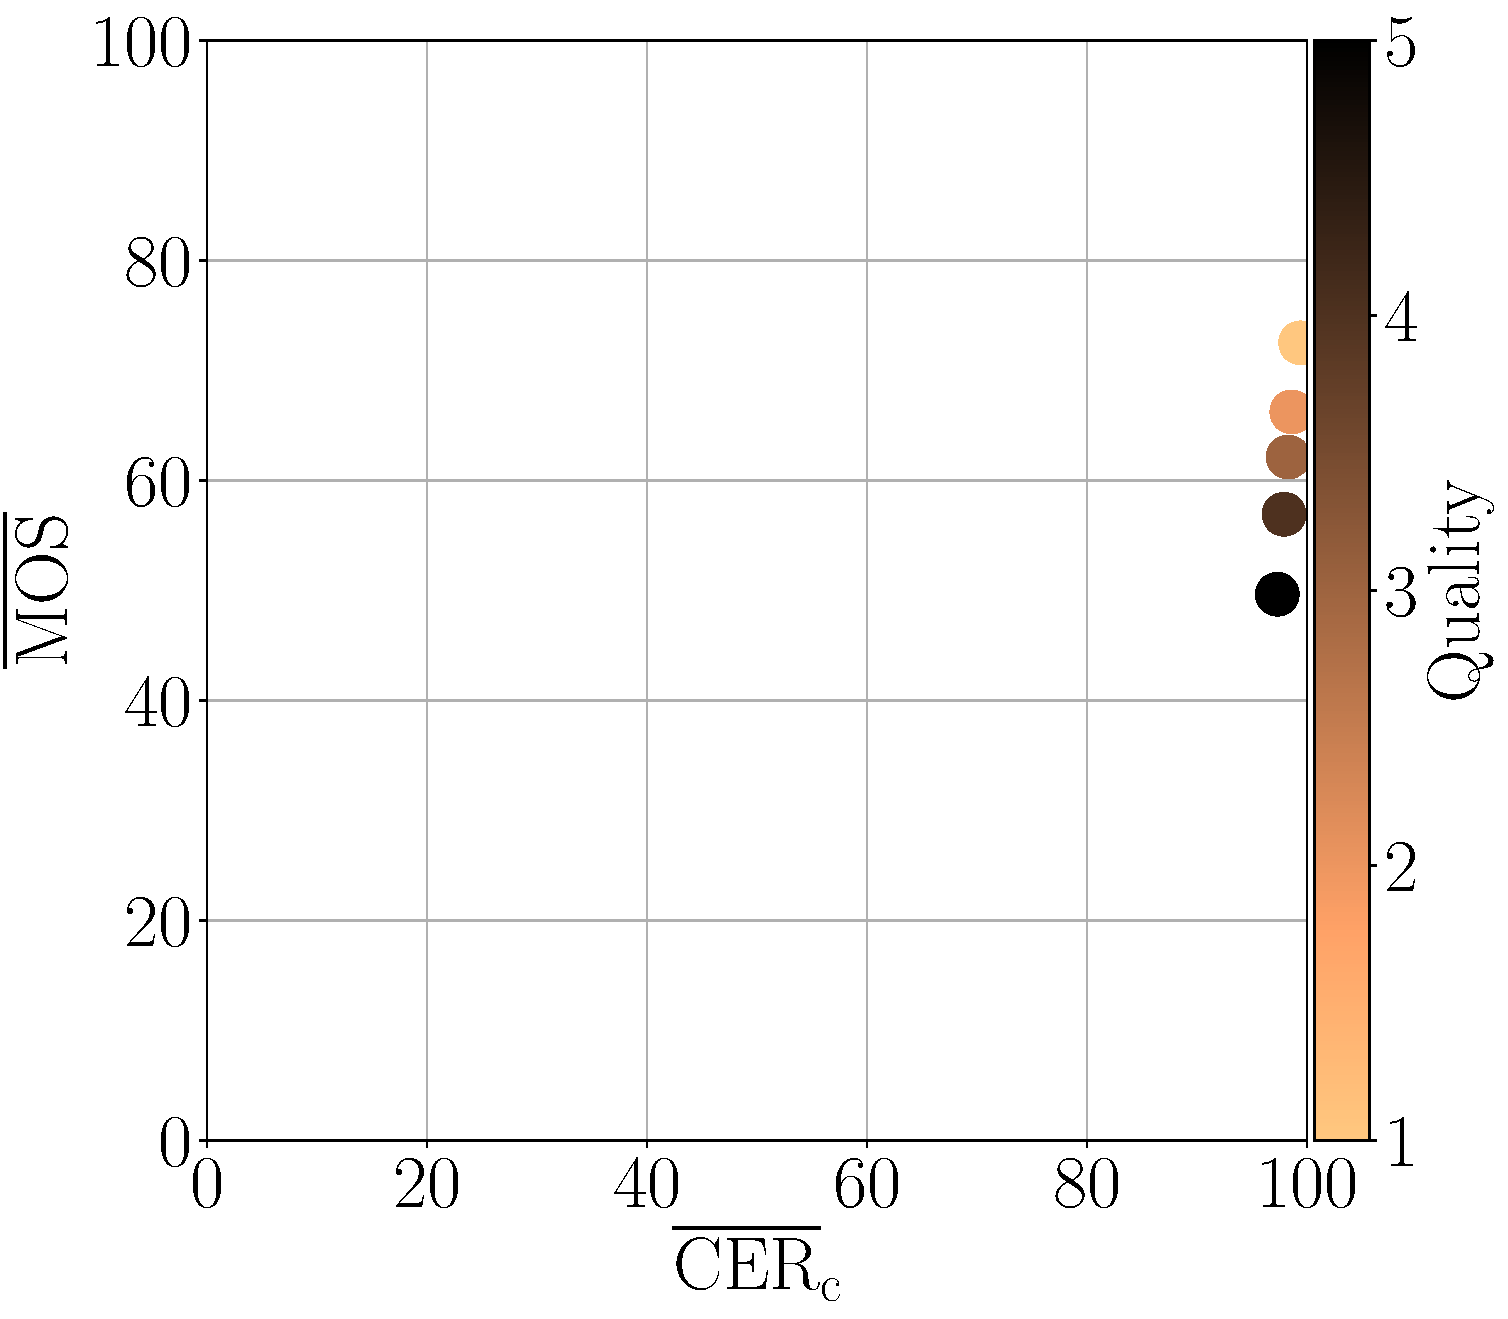
\includegraphics[width=\textwidth]{../../images/analyze/mos_cer_ref_mean_ezocr_CSC.pdf}
        \caption{CSC}
        \label{fig:mos_cer_ref_mean_ezocr_CSC}
    \end{subfigure}%
    \hfill
    \begin{subfigure}[b]{0.32\textwidth}
        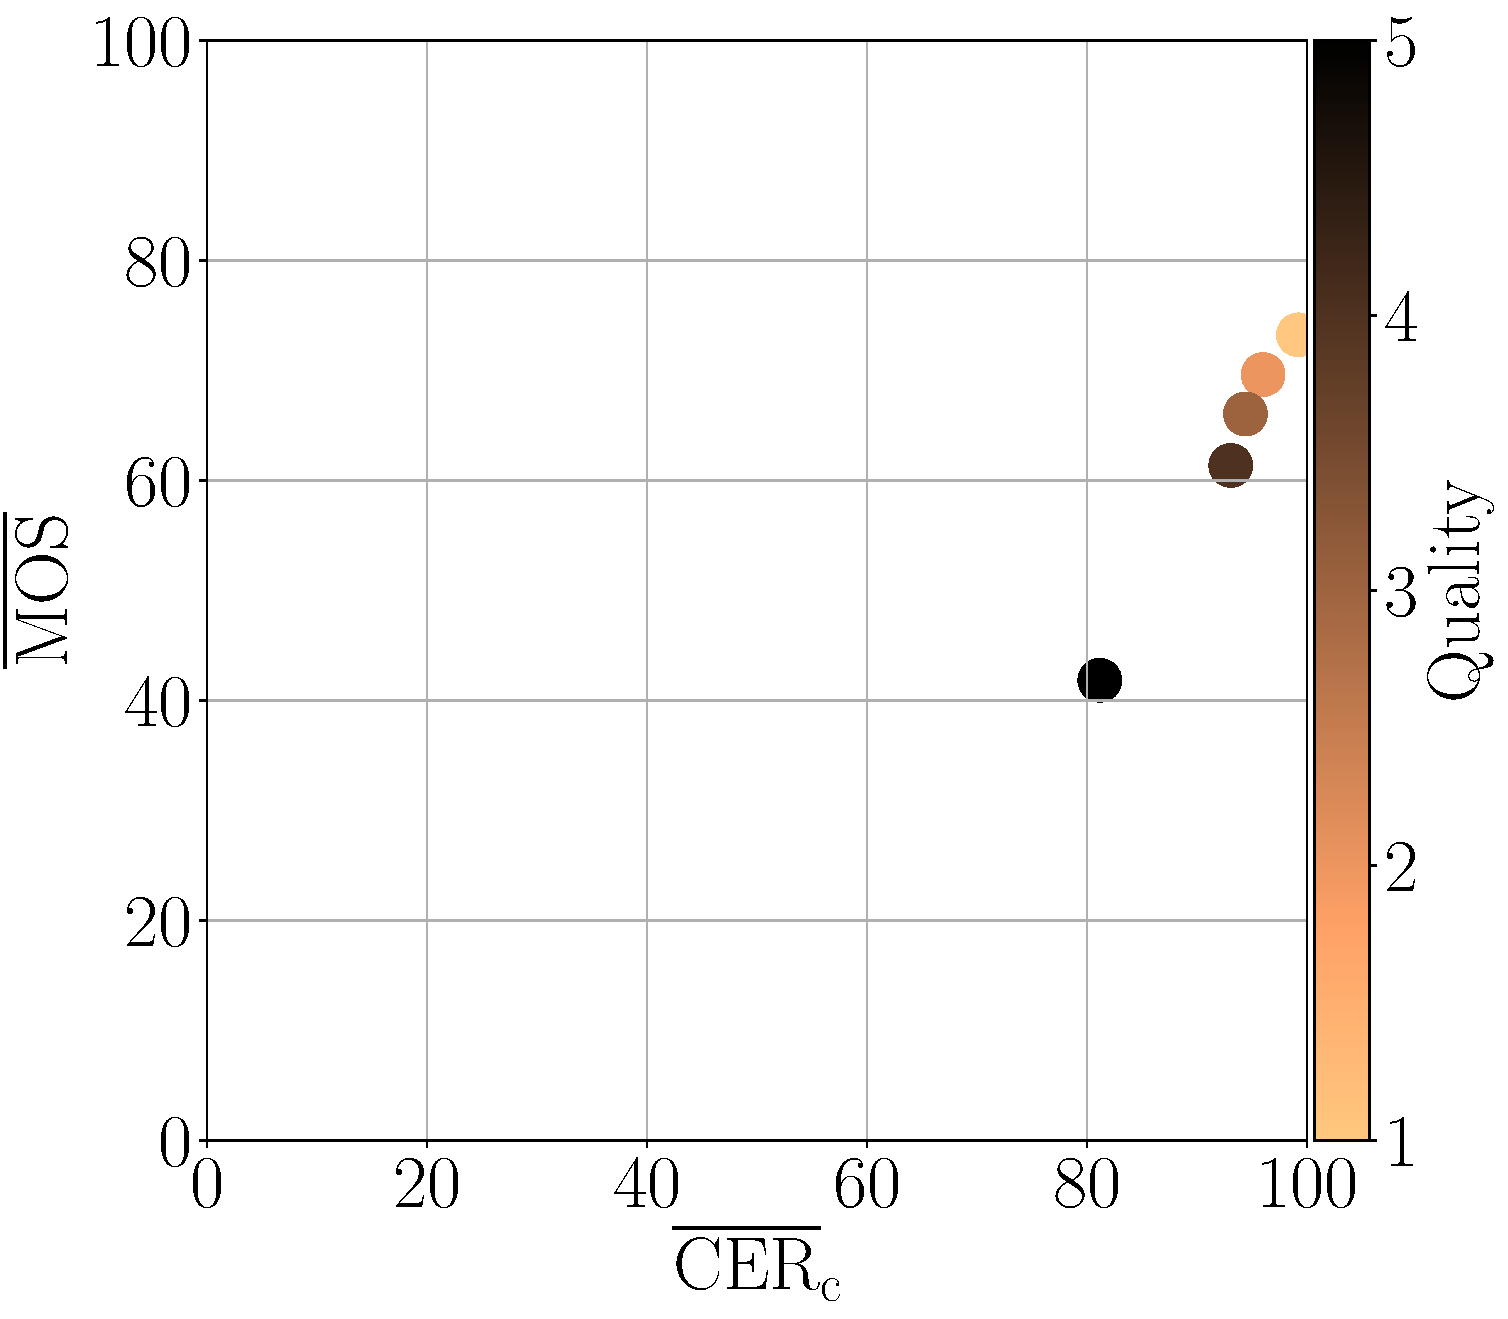
\includegraphics[width=\textwidth]{../../images/analyze/mos_cer_ref_mean_ezocr_HEVC-SCC.pdf}
        \caption{HEVC-SCC}
        \label{fig:mos_cer_ref_mean_ezocr_HEVC-SCC}
    \end{subfigure}%
    \hfill
    \begin{subfigure}[b]{0.32\textwidth}
        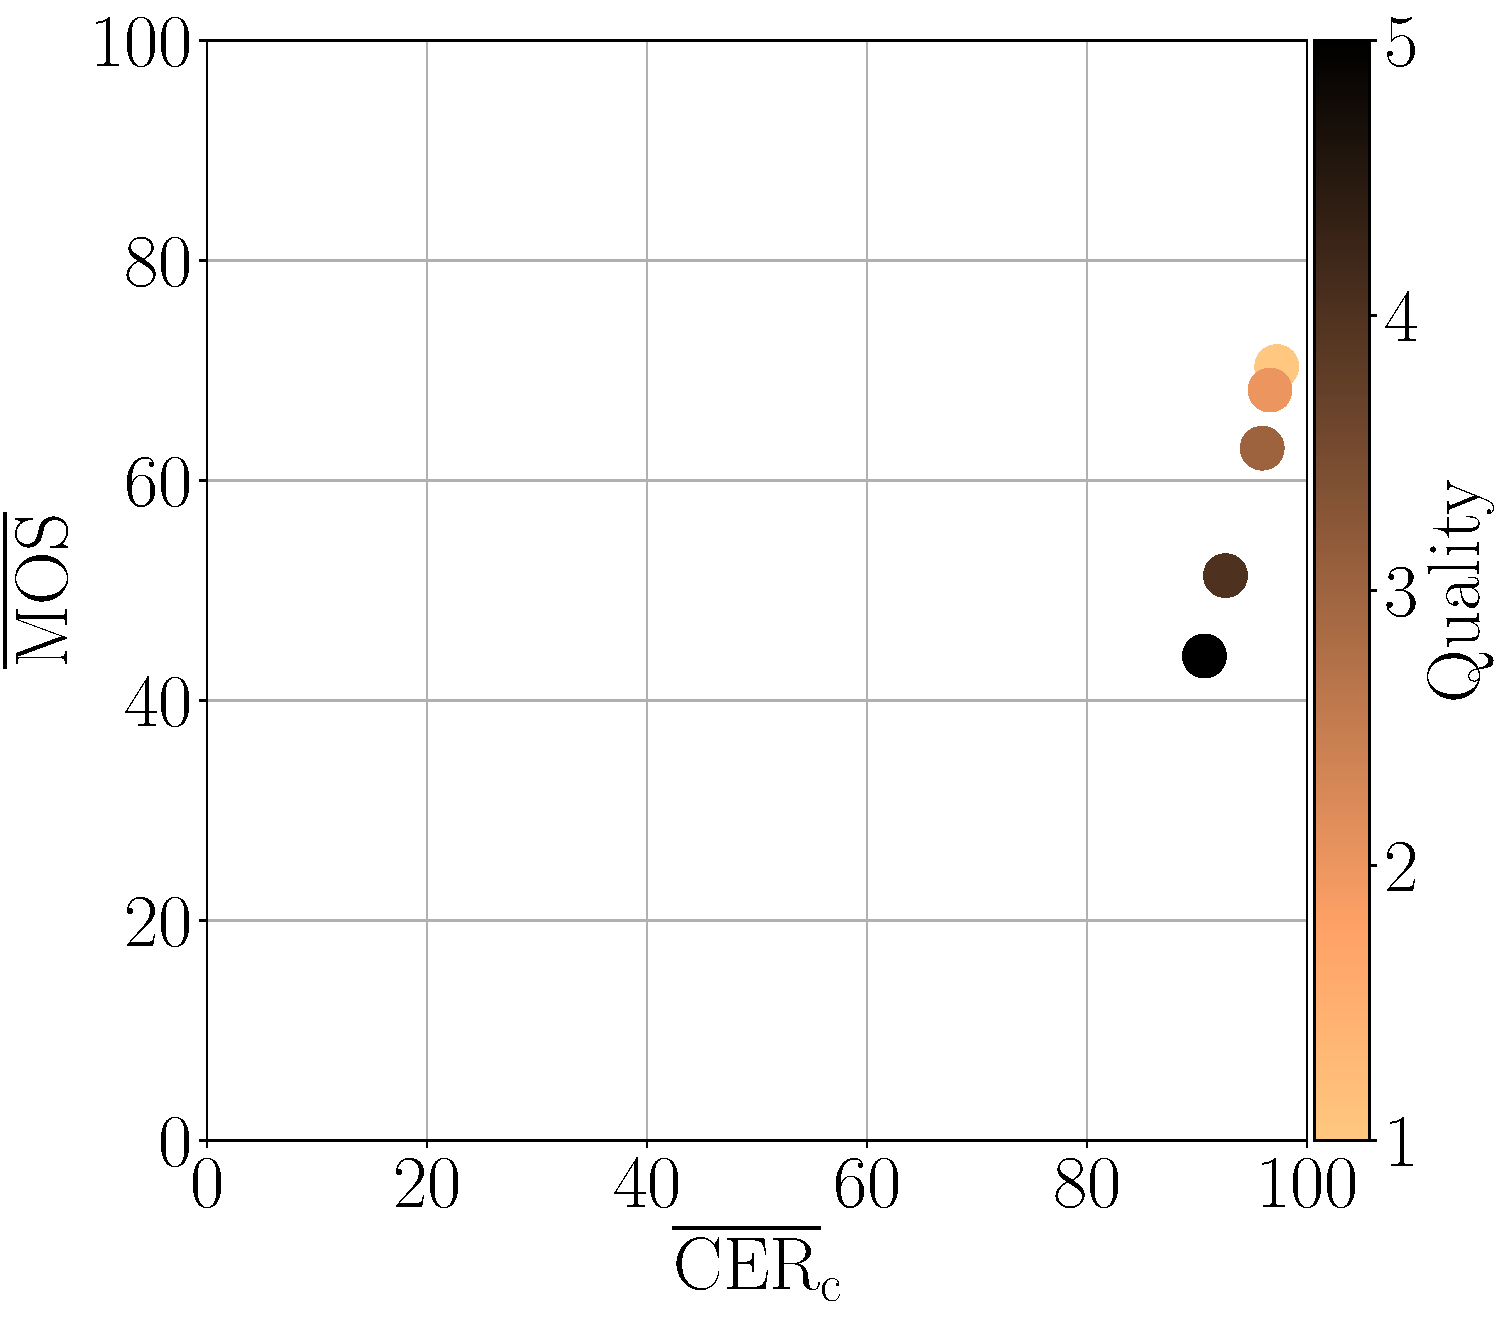
\includegraphics[width=\textwidth]{../../images/analyze/mos_cer_ref_mean_ezocr_CQD.pdf}
        \caption{CQD}
        \label{fig:mos_cer_ref_mean_ezocr_CQD}
    \end{subfigure}%
    \caption{$\overline{\text{CER}}_{\text{c}}$ in relation to the text predictions on the reference images against $\overline{\text{MOS}}$ for different distortion types with EasyOCR.}
\label{fig:mos_cer_ref_mean_ezocr}
\end{figure}

In \autoref{fig:mos_cer_ref_mean_ezocr}, we can see the $\overline{\text{CER}}_{\text{c}}$ in relation to the text predictions on the reference images against the $\overline{\text{MOS}}$ over the selected images, see \autoref{sec:dataset_analysis}, for all distortions for EasyOCR.
In general we notice that the performance ceiling for the $\overline{\text{CER}}_{\text{c}}$ is now up to almost 100.
This is due to the $\overline{\text{CER}}_{\text{c}}$ being calculated in relation to the prediction on the reference images, which is not necessarily the \gls{gt}.
The distortions \gls{csc} and \gls{cc} are not impacting the performance of EasyOCR much, like we saw in the previous section.
However, the corresponding $\overline{\text{MOS}}$ values are impacted.
For \gls{cc}, neither metric shows a clear trend.
We are uncertain why the $overline{\text{MOS}}$ for CC is not strictly decreasing with the quality level.
Contrast levels do not clearly reach from good to bad, so it might be that humans found specific contrast levels more appealing than others.
For all other distortions the graph shows a clear trend, where both $\overline{\text{CER}}_{\text{c}}$ and $\overline{\text{MOS}}$ decline with decreasing quality.
This implies at least a slight correlation between the two metrics, which we will quantify later.

% mos vs cer mean in relation to reference for Tesseract
\begin{figure}[h!]
\centering
    \begin{subfigure}[b]{0.32\textwidth}
        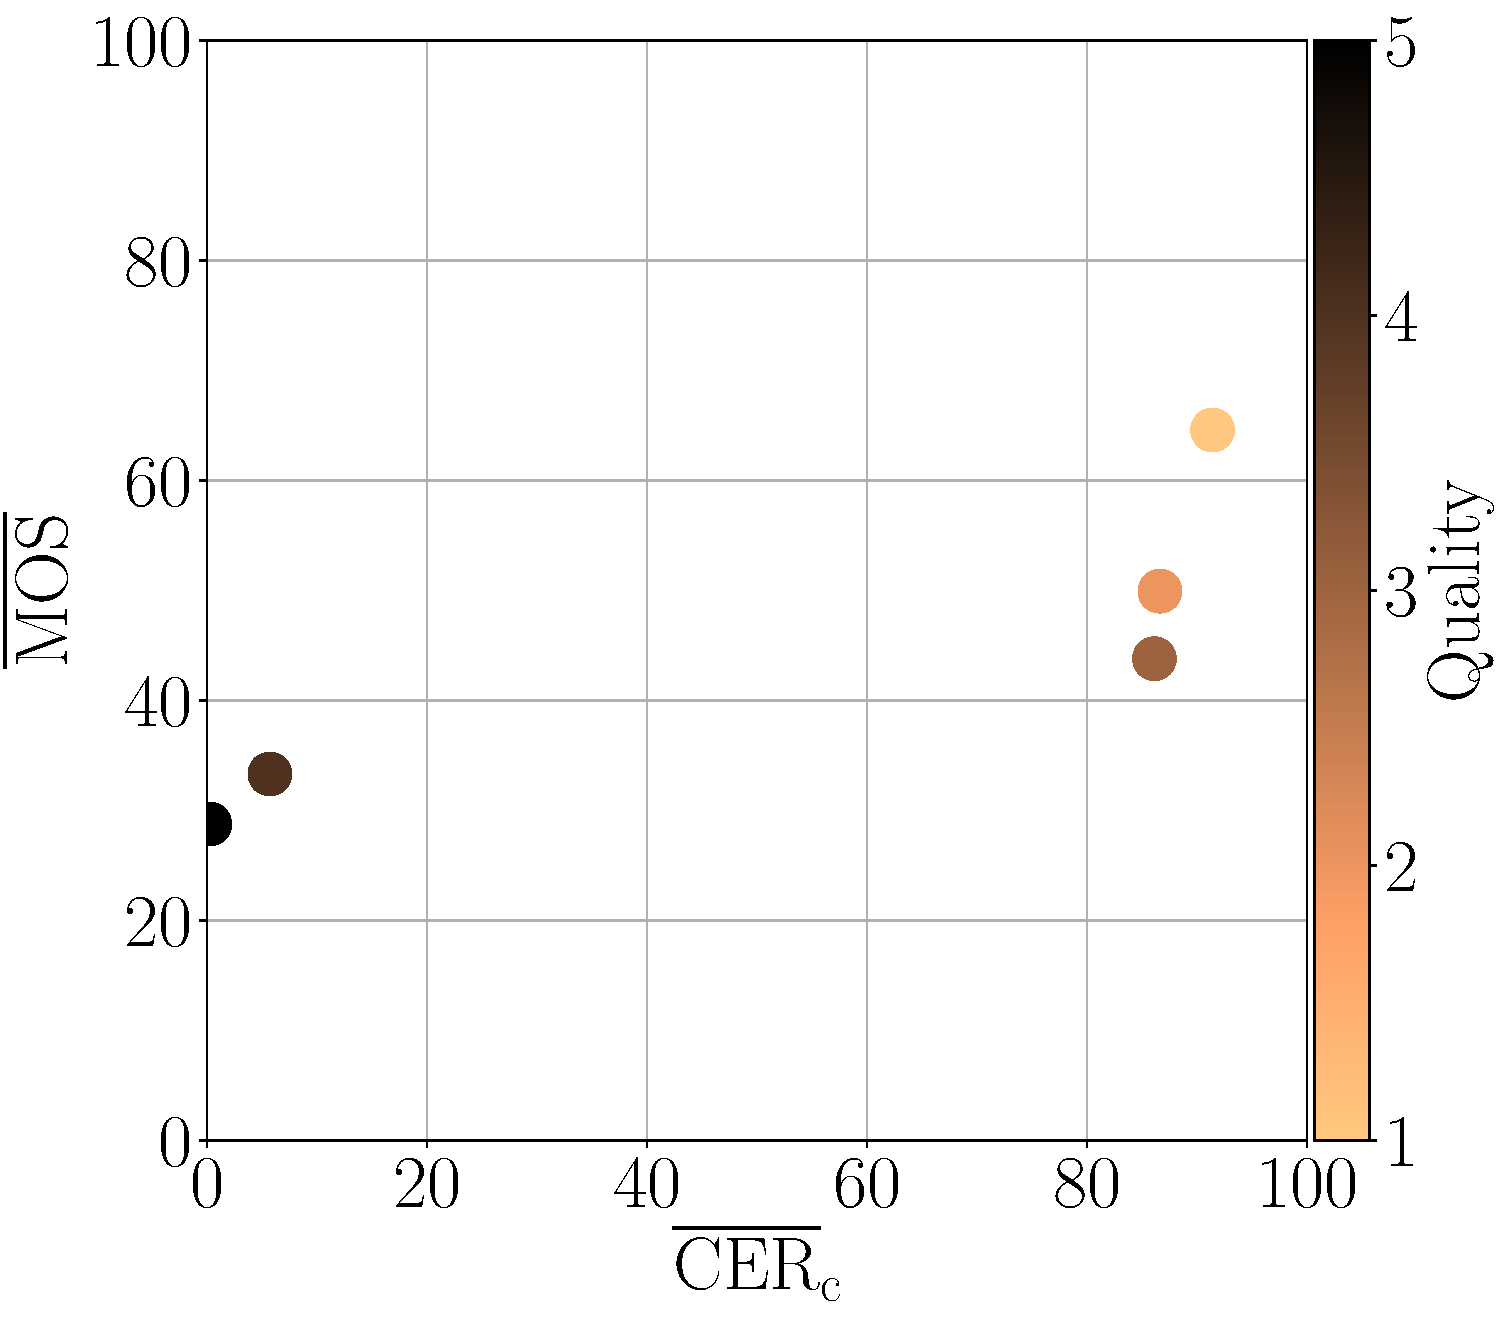
\includegraphics[width=\textwidth]{../../images/analyze/mos_cer_ref_mean_tess_GN.pdf}
        \caption{GN}
        \label{fig:mos_cer_ref_mean_tess_GN}
    \end{subfigure}%
    \hfill
    \begin{subfigure}[b]{0.32\textwidth}
        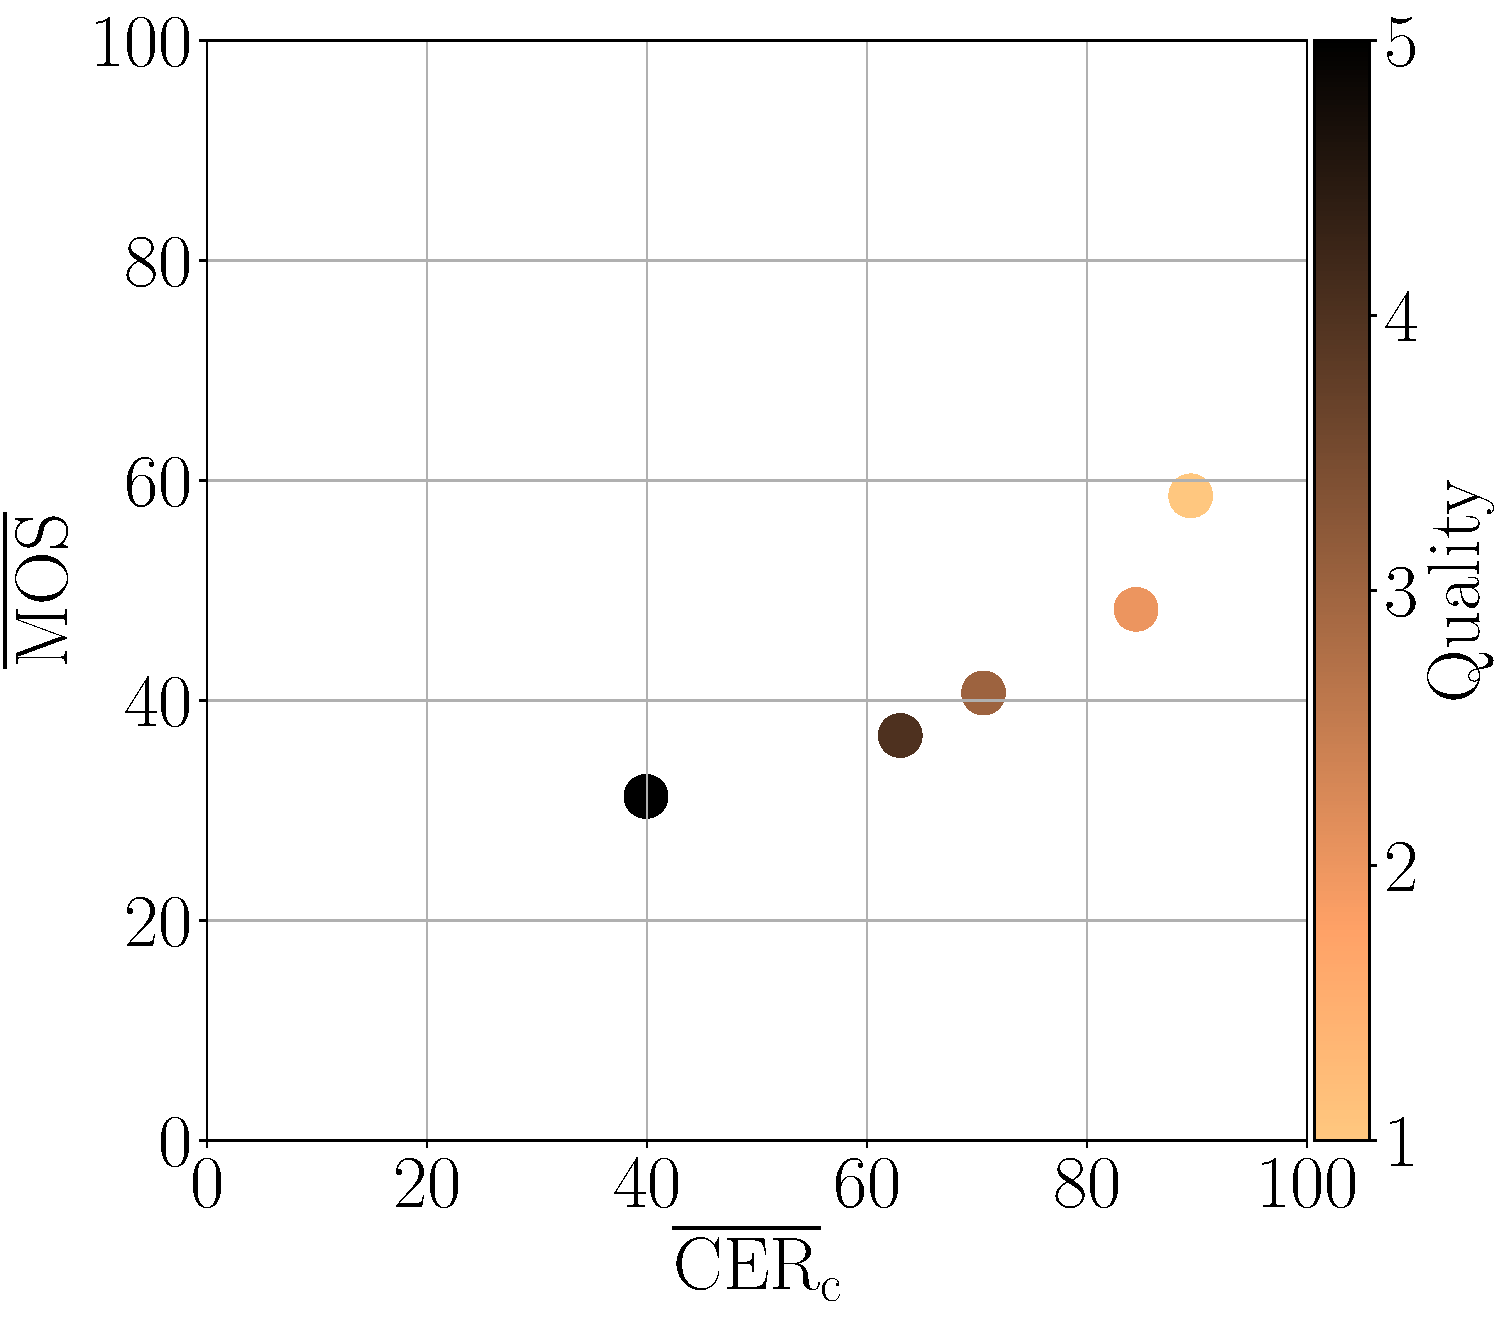
\includegraphics[width=\textwidth]{../../images/analyze/mos_cer_ref_mean_tess_GB.pdf}
        \caption{GB}
        \label{fig:mos_cer_ref_mean_tess_GB}
    \end{subfigure}%
    \hfill
    \begin{subfigure}[b]{0.32\textwidth}
        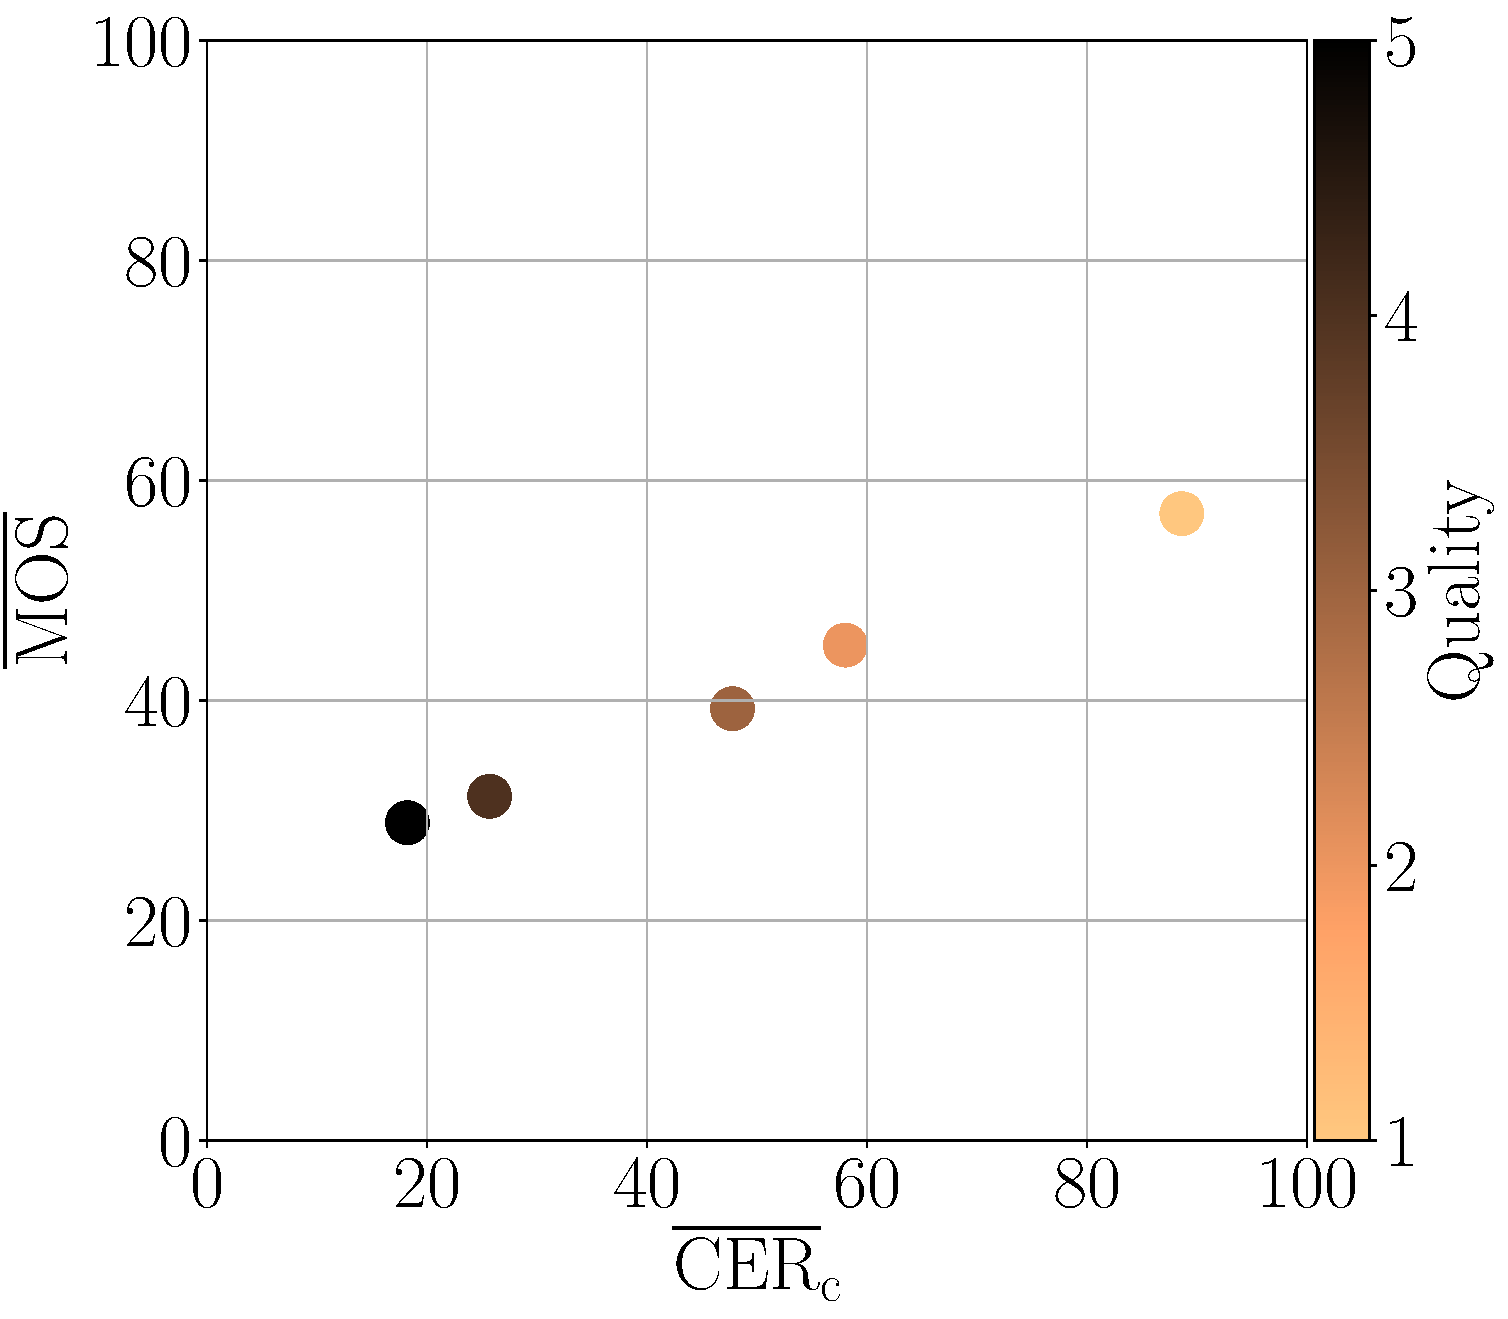
\includegraphics[width=\textwidth]{../../images/analyze/mos_cer_ref_mean_tess_MB.pdf}
        \caption{MB}
        \label{fig:mos_cer_ref_mean_tess_MB}
    \end{subfigure}%
    \newline
    \begin{subfigure}[b]{0.32\textwidth}
        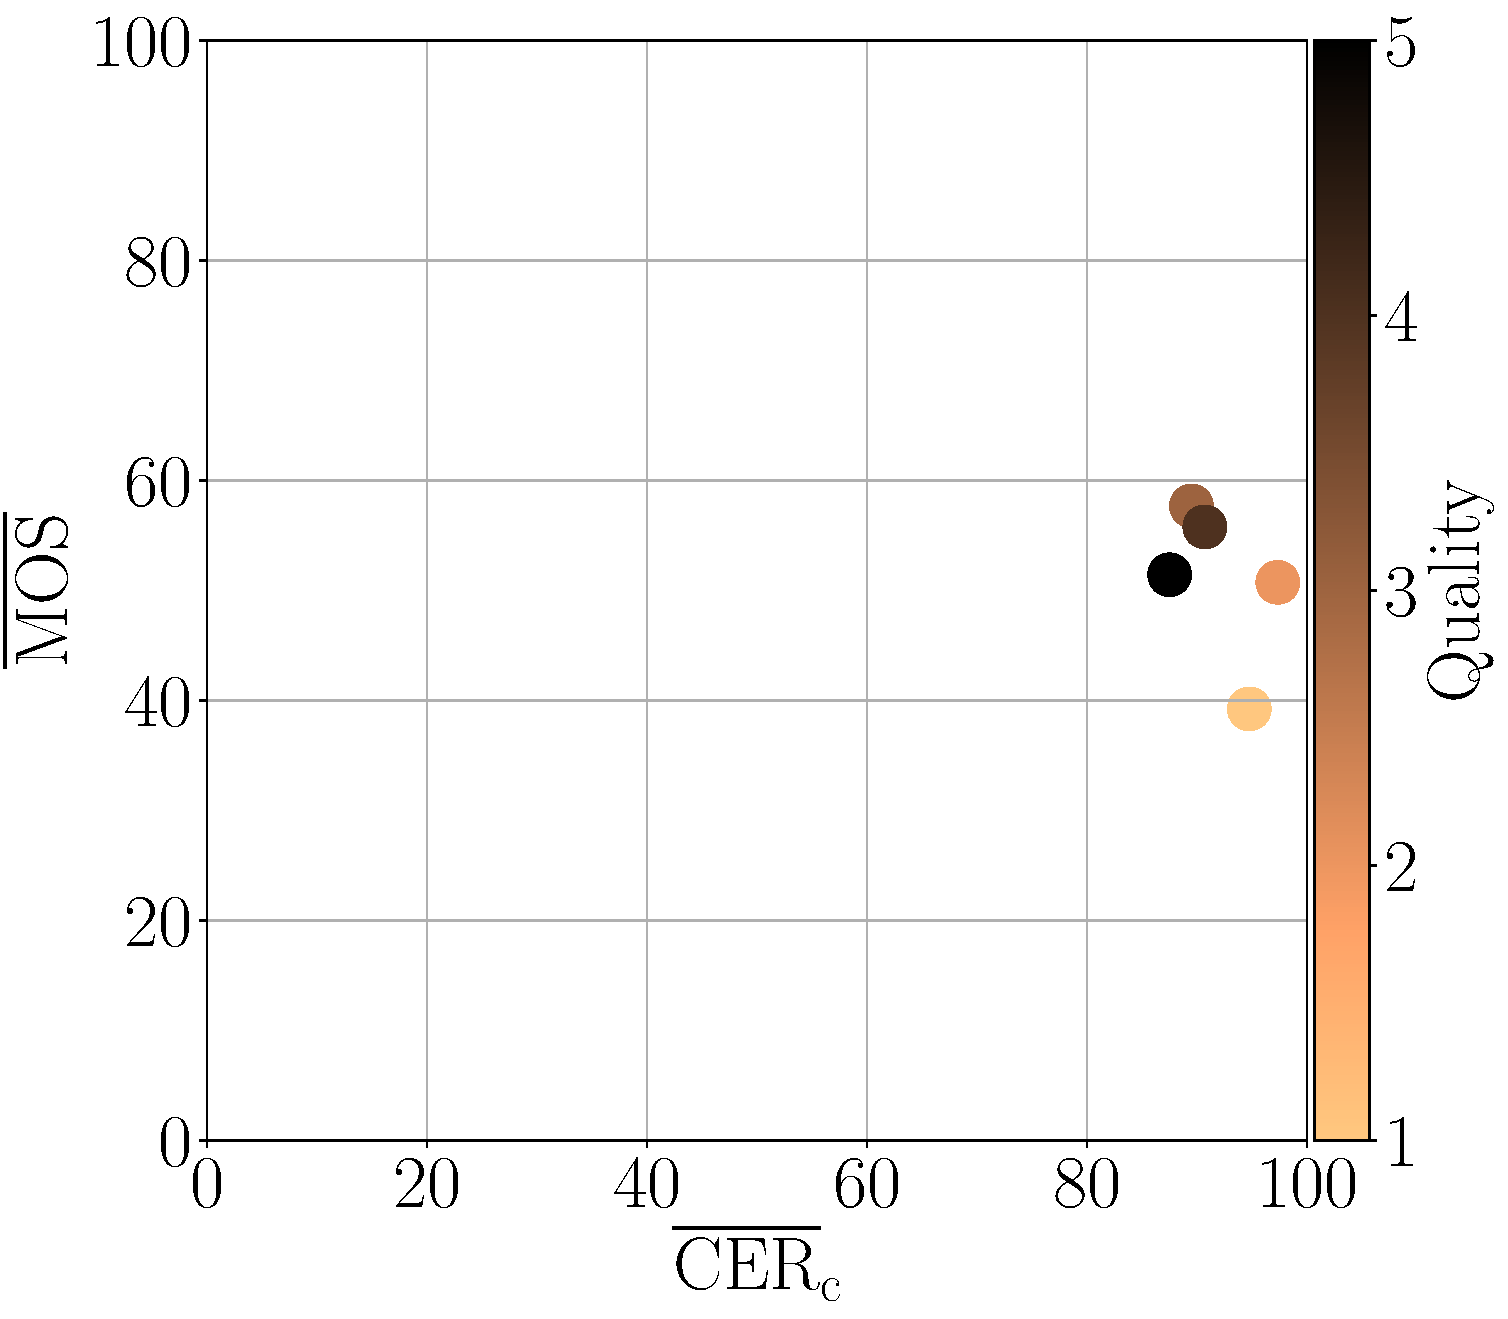
\includegraphics[width=\textwidth]{../../images/analyze/mos_cer_ref_mean_tess_CC.pdf}
        \caption{CC}
        \label{fig:mos_cer_ref_mean_tess_CC}
    \end{subfigure}%
    \hfill
    \begin{subfigure}[b]{0.32\textwidth}
        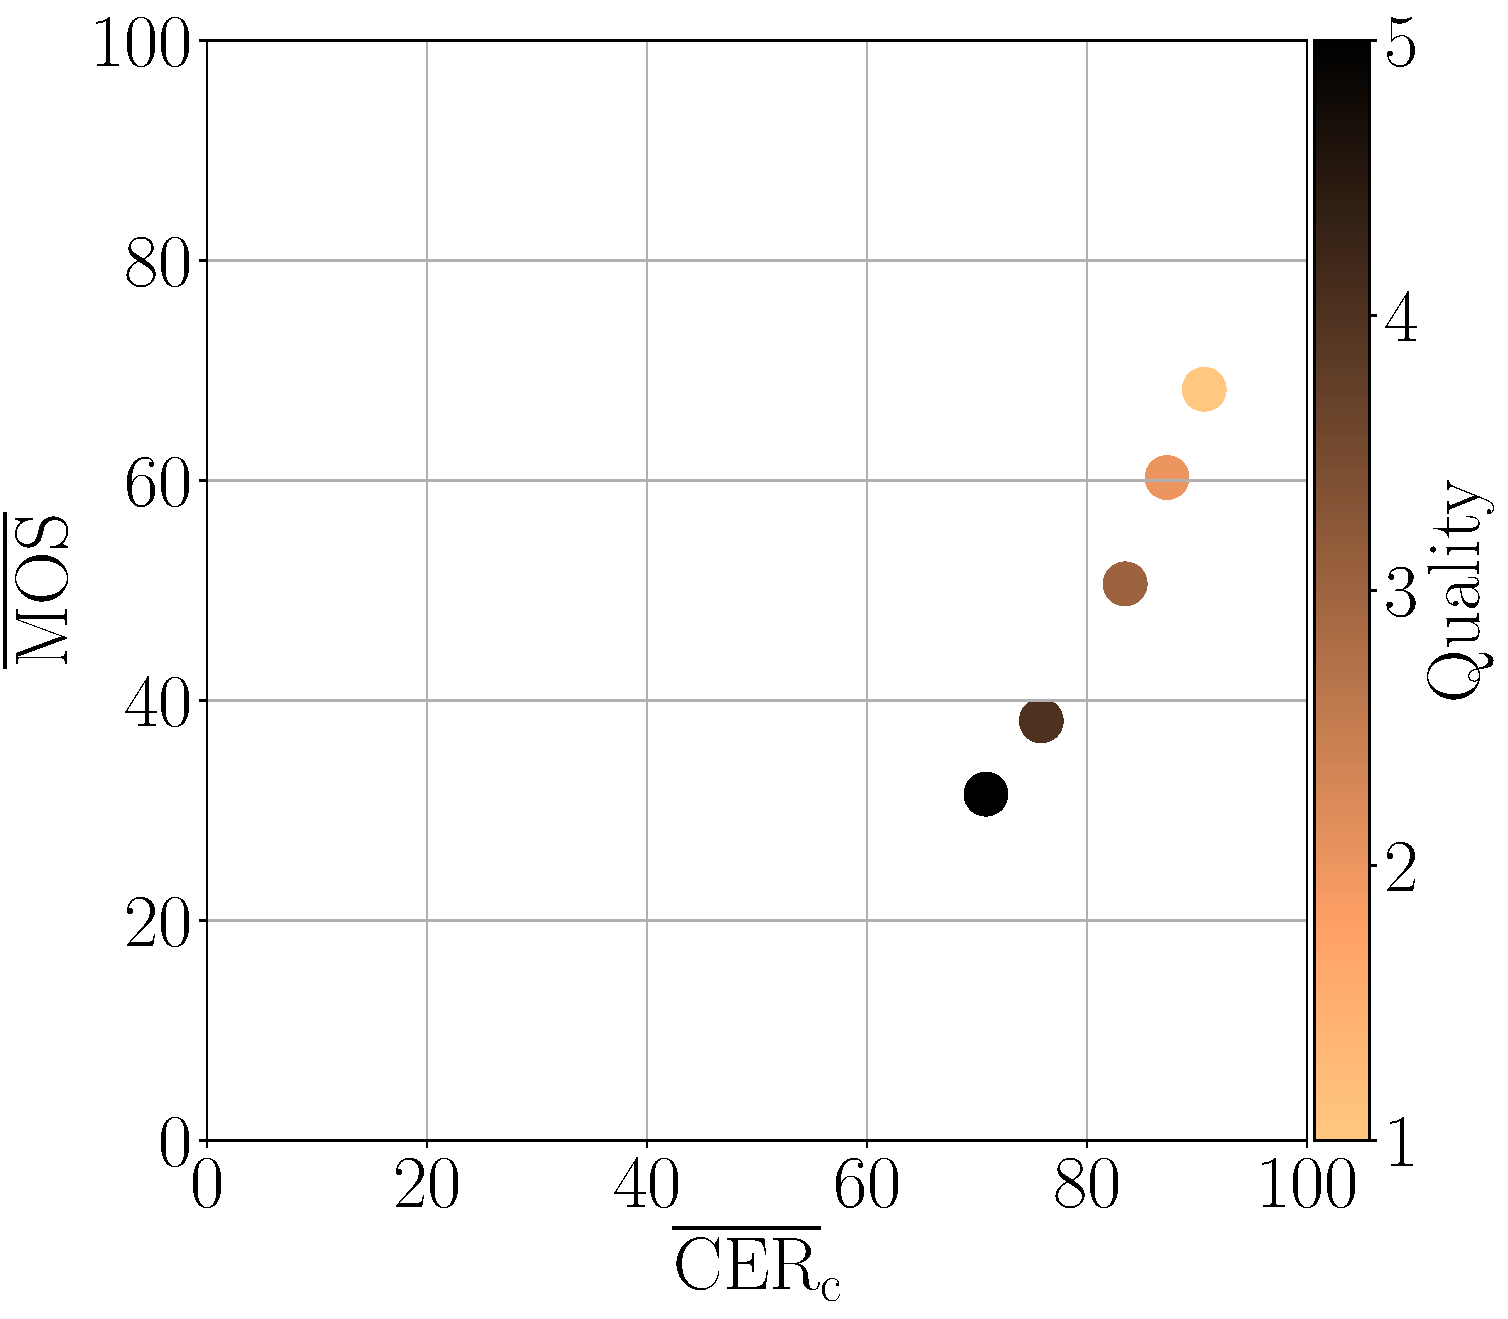
\includegraphics[width=\textwidth]{../../images/analyze/mos_cer_ref_mean_tess_JPEG.pdf}
        \caption{JPEG}
        \label{fig:mos_cer_ref_mean_tess_JPEG}
    \end{subfigure}%
    \hfill
    \begin{subfigure}[b]{0.32\textwidth}
        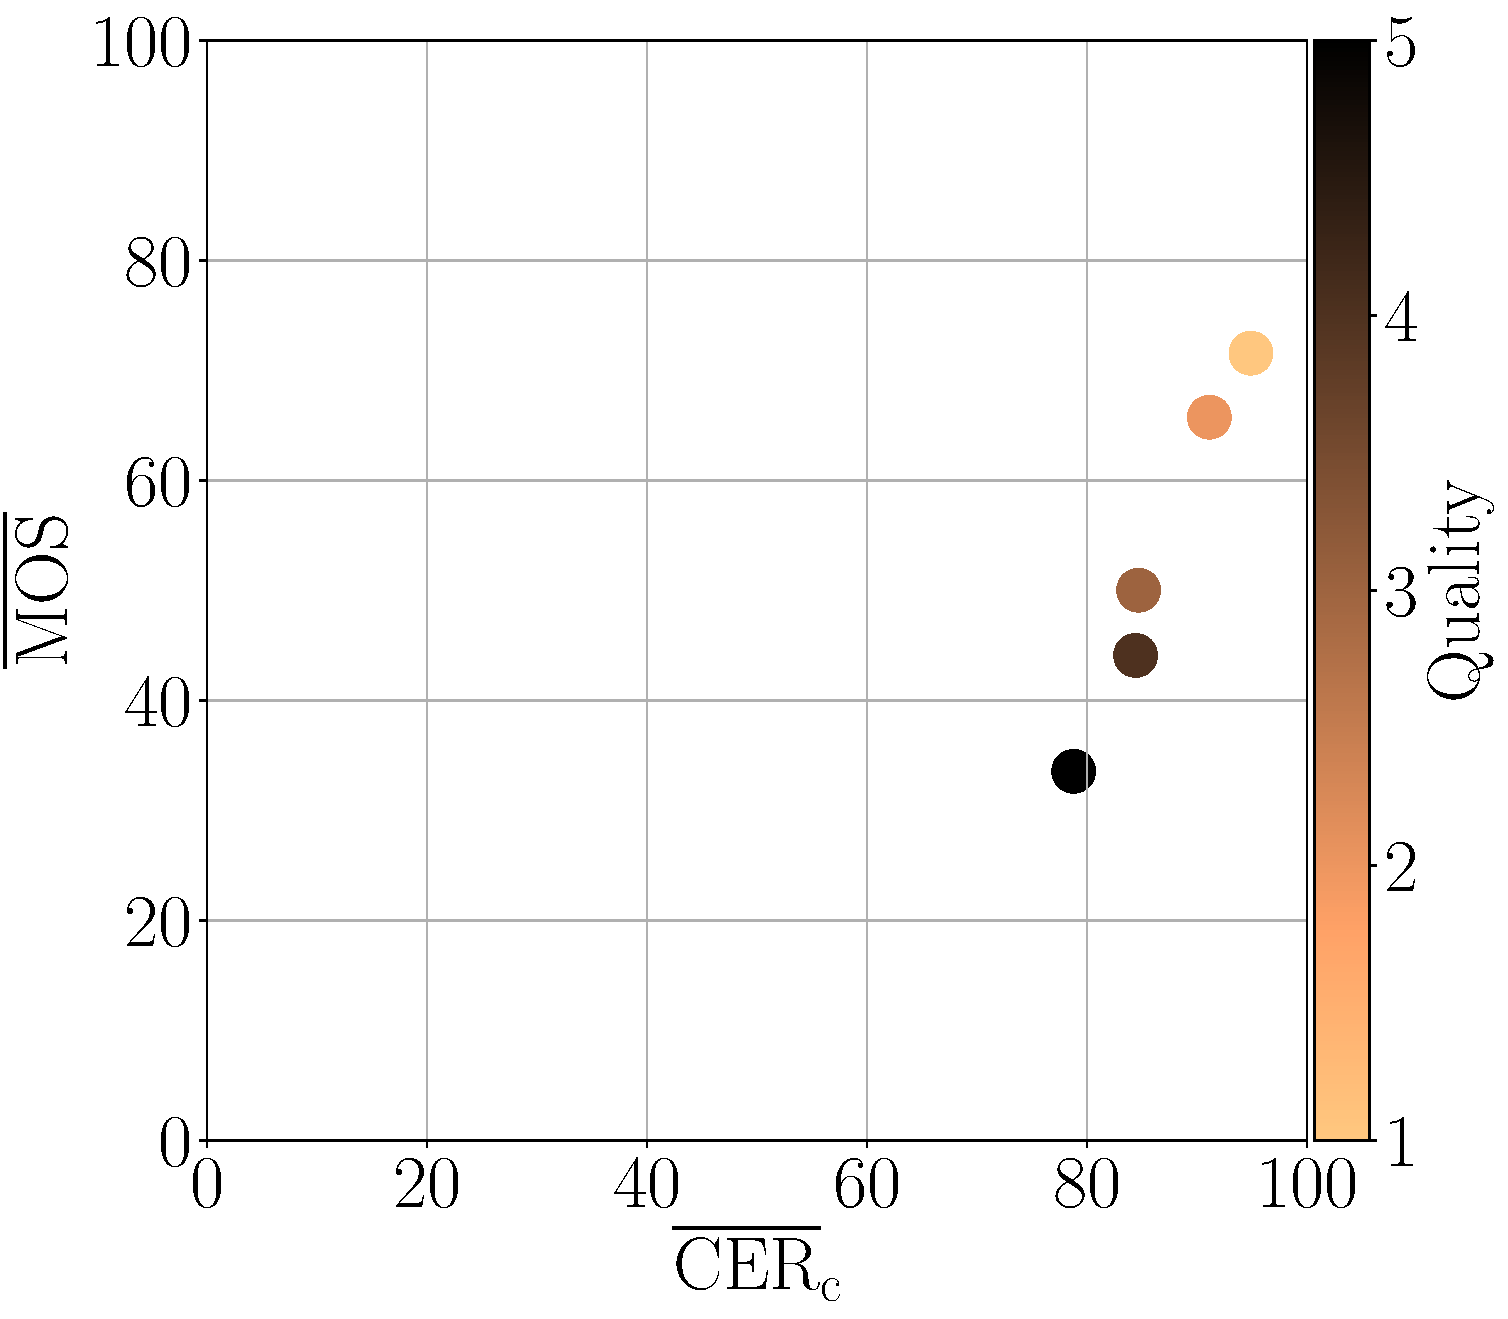
\includegraphics[width=\textwidth]{../../images/analyze/mos_cer_ref_mean_tess_JPEG2000.pdf}
        \caption{JPEG2000}
        \label{fig:mos_cer_ref_mean_tess_JPEG2000}
    \end{subfigure}%
    \newline
    \begin{subfigure}[b]{0.32\textwidth}
        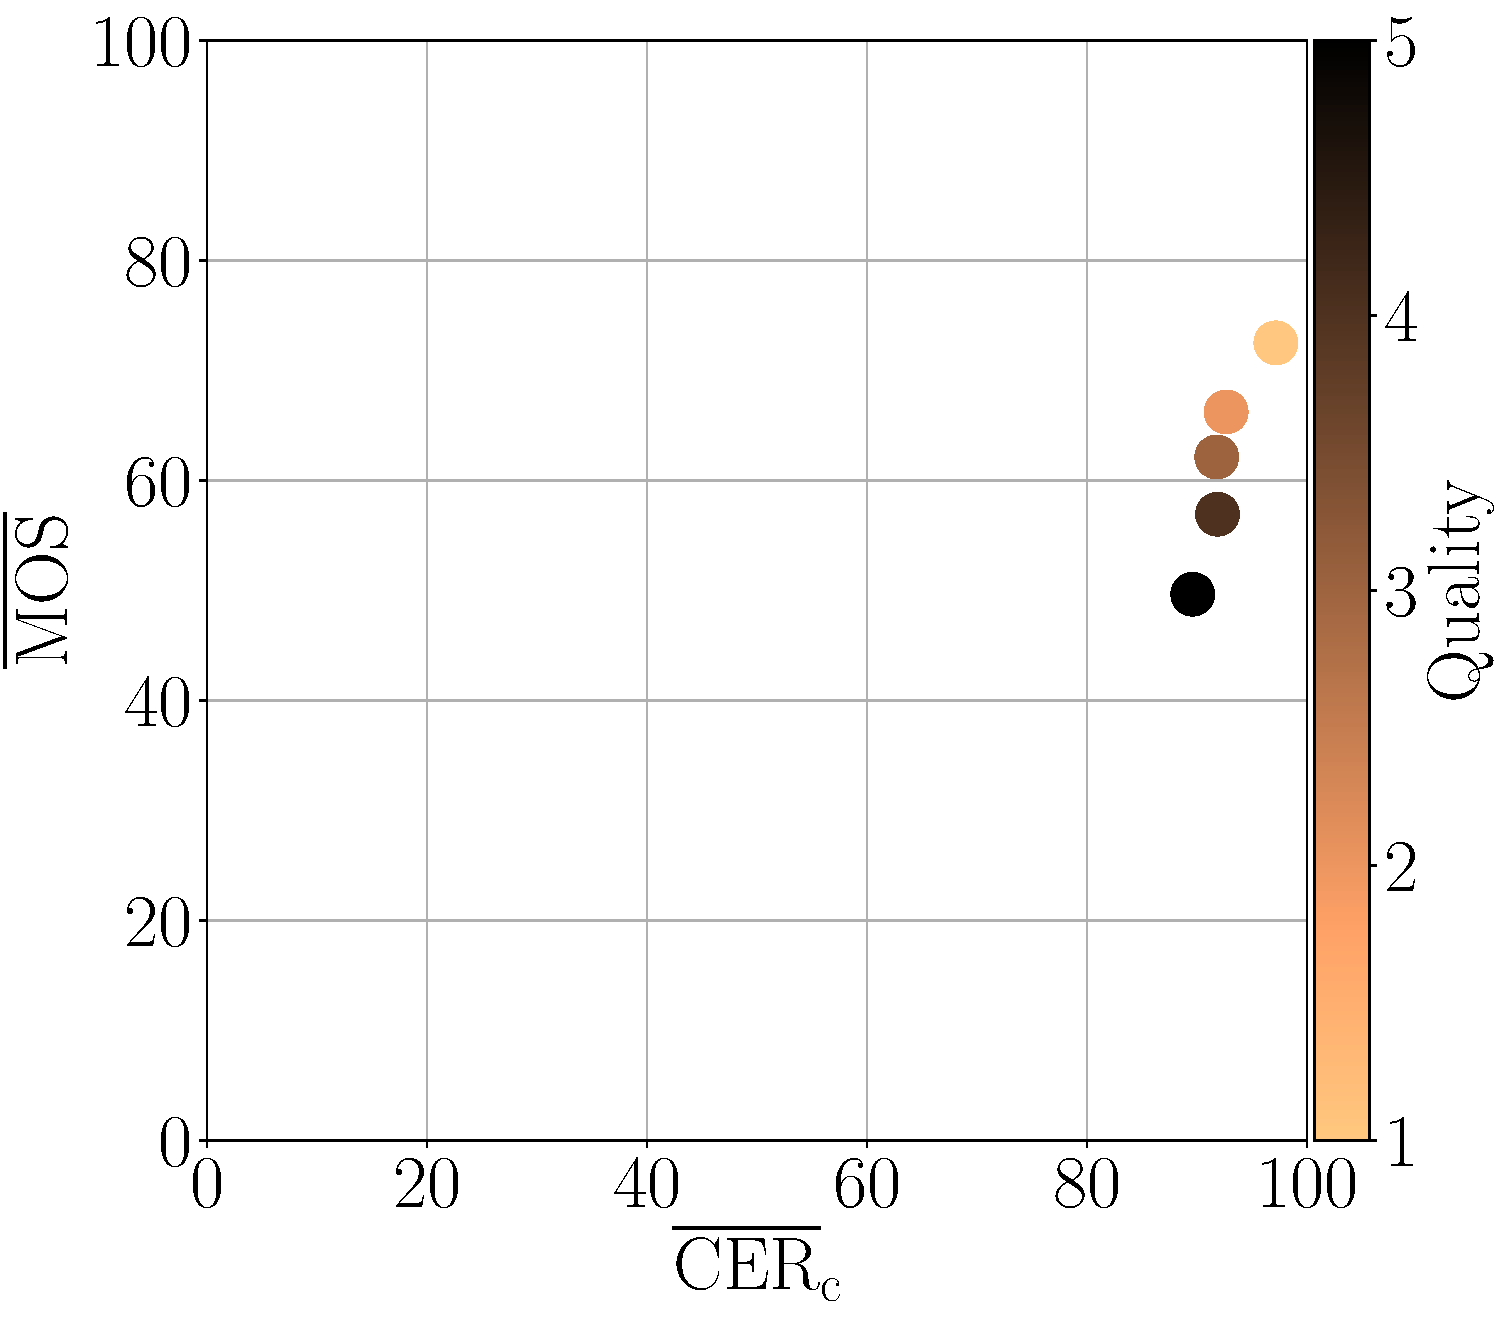
\includegraphics[width=\textwidth]{../../images/analyze/mos_cer_ref_mean_tess_CSC.pdf}
        \caption{CSC}
        \label{fig:mos_cer_ref_mean_tess_CSC}
    \end{subfigure}%
    \hfill
    \begin{subfigure}[b]{0.32\textwidth}
        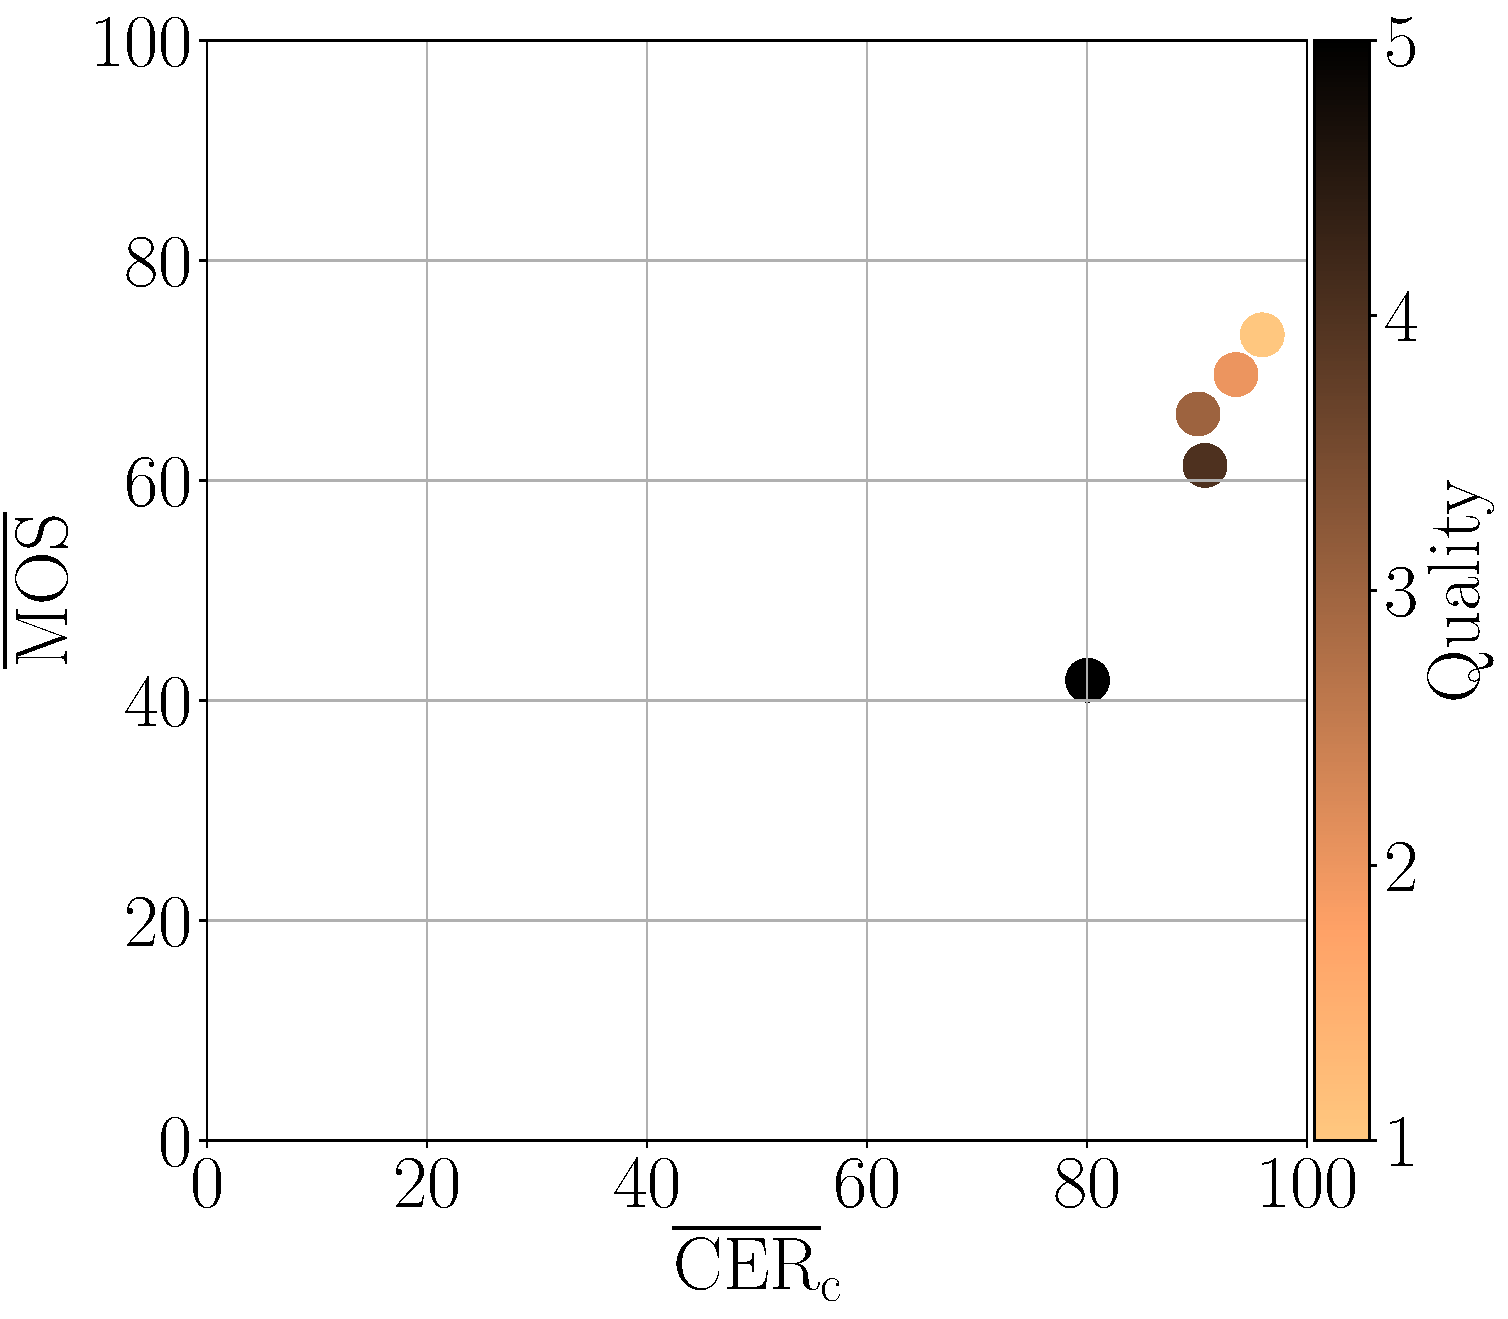
\includegraphics[width=\textwidth]{../../images/analyze/mos_cer_ref_mean_tess_HEVC-SCC.pdf}
        \caption{HEVC-SCC}
        \label{fig:mos_cer_ref_mean_tess_HEVC-SCC}
    \end{subfigure}%
    \hfill
    \begin{subfigure}[b]{0.32\textwidth}
        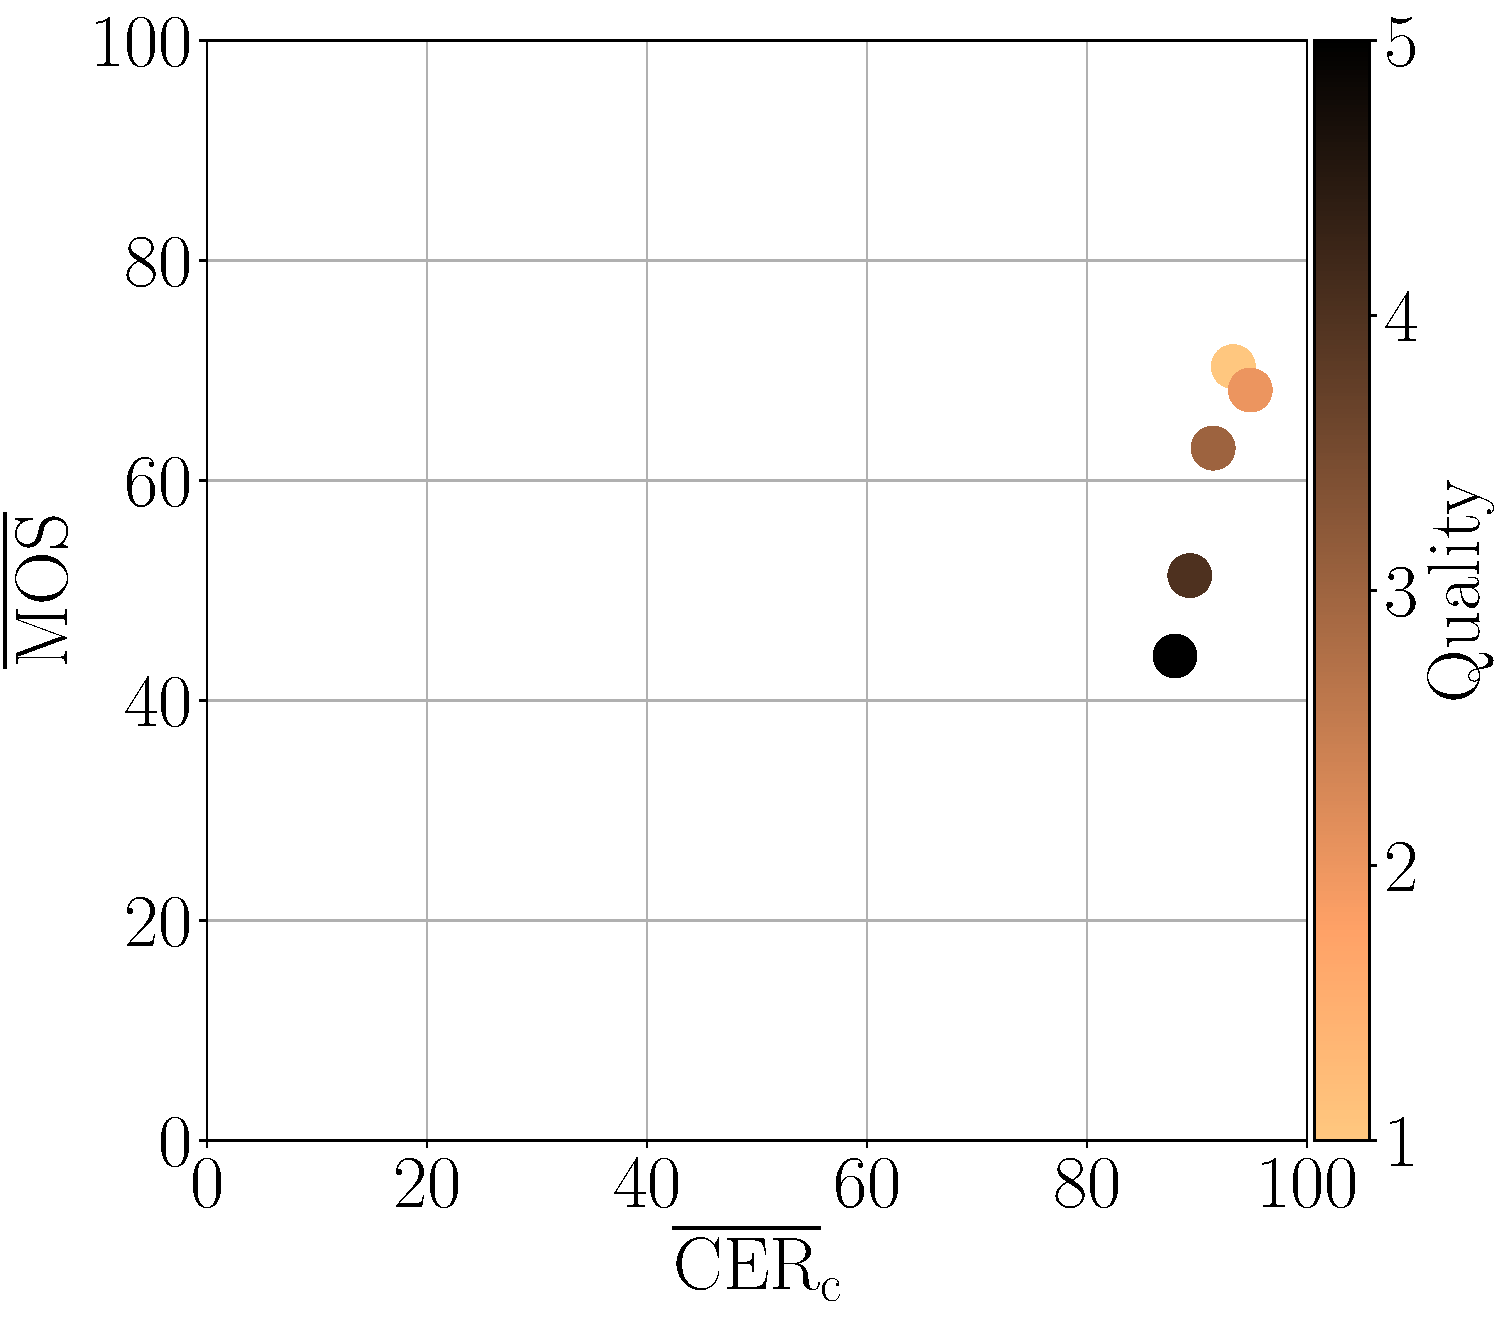
\includegraphics[width=\textwidth]{../../images/analyze/mos_cer_ref_mean_tess_CQD.pdf}
        \caption{CQD}
        \label{fig:mos_cer_ref_mean_tess_CQD}
    \end{subfigure}%
    \caption{$\overline{\text{CER}}_{\text{c}}$ in relation to the text predictions on the reference images against $\overline{\text{MOS}}$ for different distortion types with Tesseract \gls{ocr}.}
\label{fig:mos_cer_ref_mean_tess}
\end{figure}

In \autoref{fig:mos_cer_ref_mean_tess}, we conduct the same analysis for Tesseract.
Tesseract \gls{ocr} performs generally worse on all distortions compared to EasyOCR.
Due to the $\overline{\text{MOS}}$ being generally lower than the $\overline{\text{CER}}_{\text{c}}$, for some distortions the $\text{CER}_{\text{c}}$ from Tesseract \gls{ocr} might exhibit a higher correlation with the \gls{mos}.
For \gls{jpeg} for example, Tesseract's performance seems almost perfectly linear, compared to EasyOCR's nonlinear performance.
We can clearly see that the $\overline{\text{CER}}_{\text{c}}$ drops sharply on quality levels 4 and 5 of \gls{gn} while the $\overline{\text{MOS}}$ does not.
Such a large drop is not representative of the trend of the \gls{mos} and is therefore not desirable.


In general however, we need to be careful, as we are only considering the mean values of the $\text{CER}_{\text{c}}$ and \gls{mos}.
For a full analysis the full distribution of the metrics needs to be considered.
In the next part, we will consider all datapoints separately.
Additionally, we fit a model to the data points to remove nonlinearities from the objective values as described in \autoref{subsec:nonlinear}.




% mos vs cer (fitted) mean in relation to reference for ezocr
\begin{figure}[h!]
\centering
    \begin{subfigure}[b]{0.32\textwidth}
        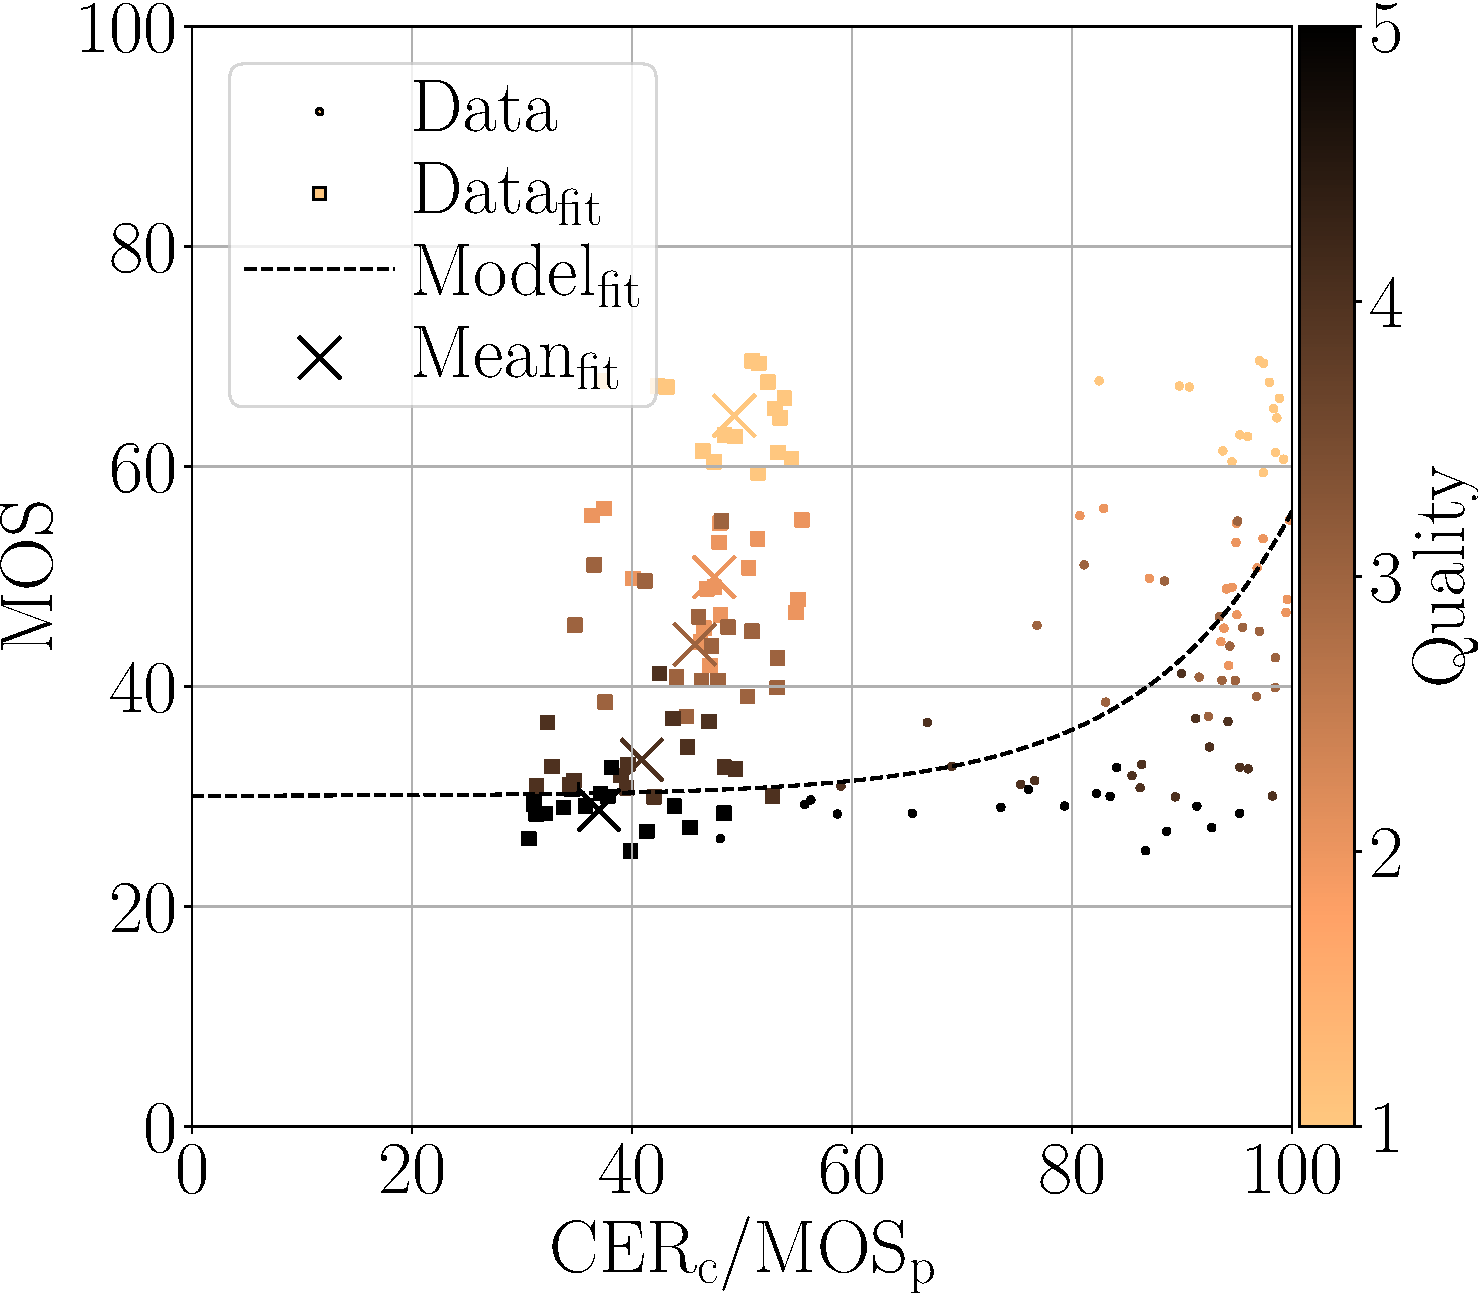
\includegraphics[width=\textwidth]{../../images/analyze/mos_cer_ref_fitted_mean_ezocr_GN.pdf}
        \caption{GN}
        \label{fig:mos_cer_ref_fitted_mean_ezocr_GN}
    \end{subfigure}%
    \hfill
    \begin{subfigure}[b]{0.32\textwidth}
        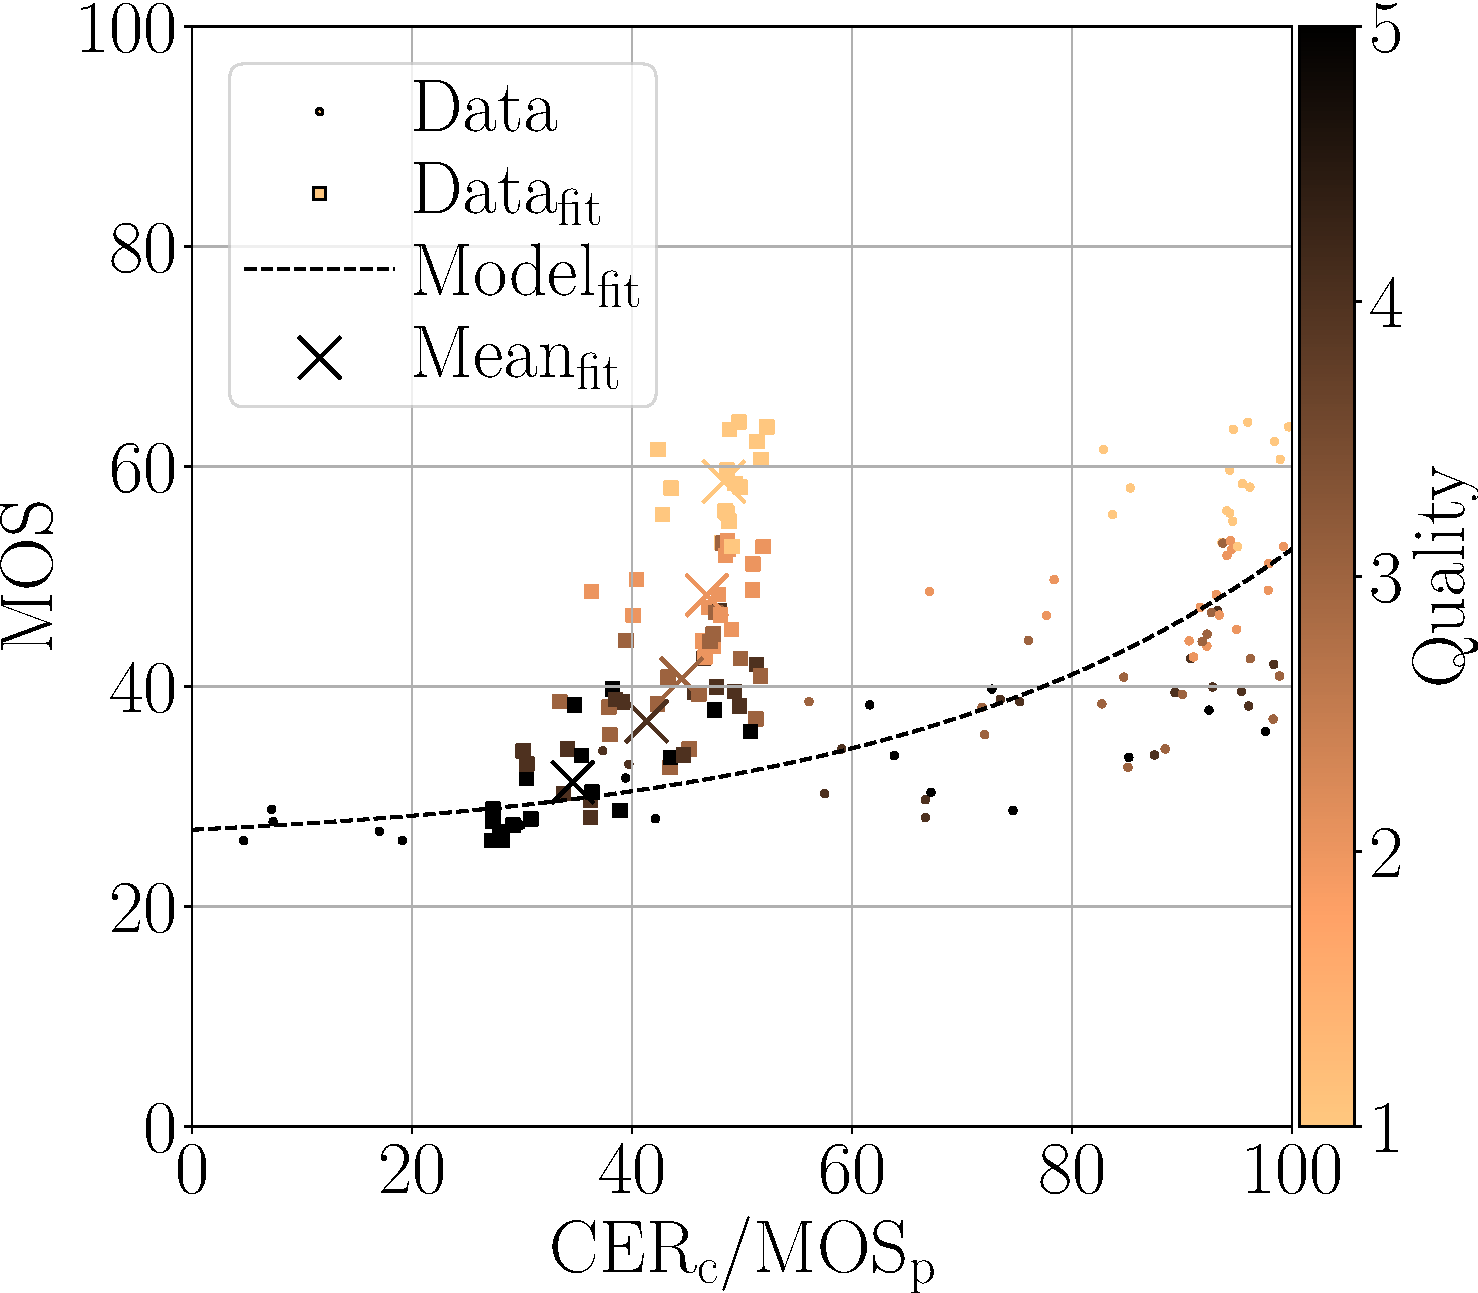
\includegraphics[width=\textwidth]{../../images/analyze/mos_cer_ref_fitted_mean_ezocr_GB.pdf}
        \caption{GB}
        \label{fig:mos_cer_ref_fitted_mean_ezocr_GB}
    \end{subfigure}%
    \hfill
    \begin{subfigure}[b]{0.32\textwidth}
        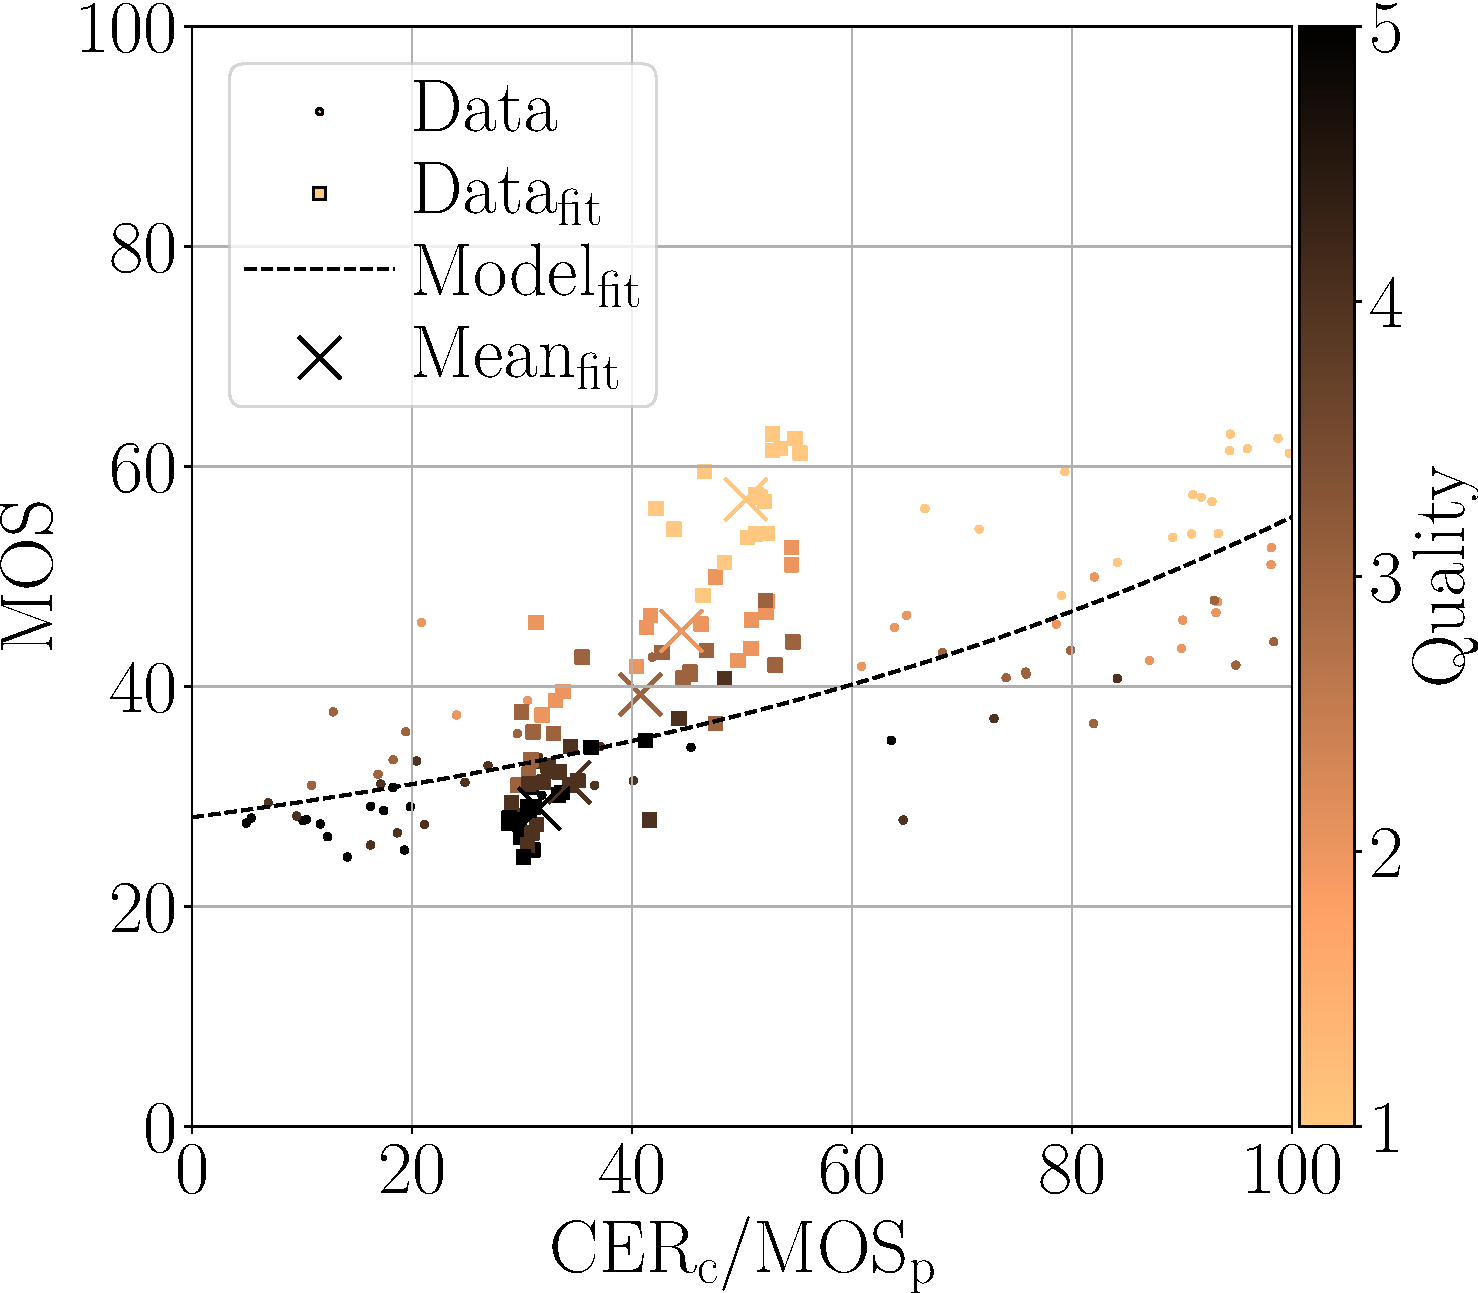
\includegraphics[width=\textwidth]{../../images/analyze/mos_cer_ref_fitted_mean_ezocr_MB.pdf}
        \caption{MB}
        \label{fig:mos_cer_ref_fitted_mean_ezocr_MB}
    \end{subfigure}%
    \newline
    \begin{subfigure}[b]{0.32\textwidth}
        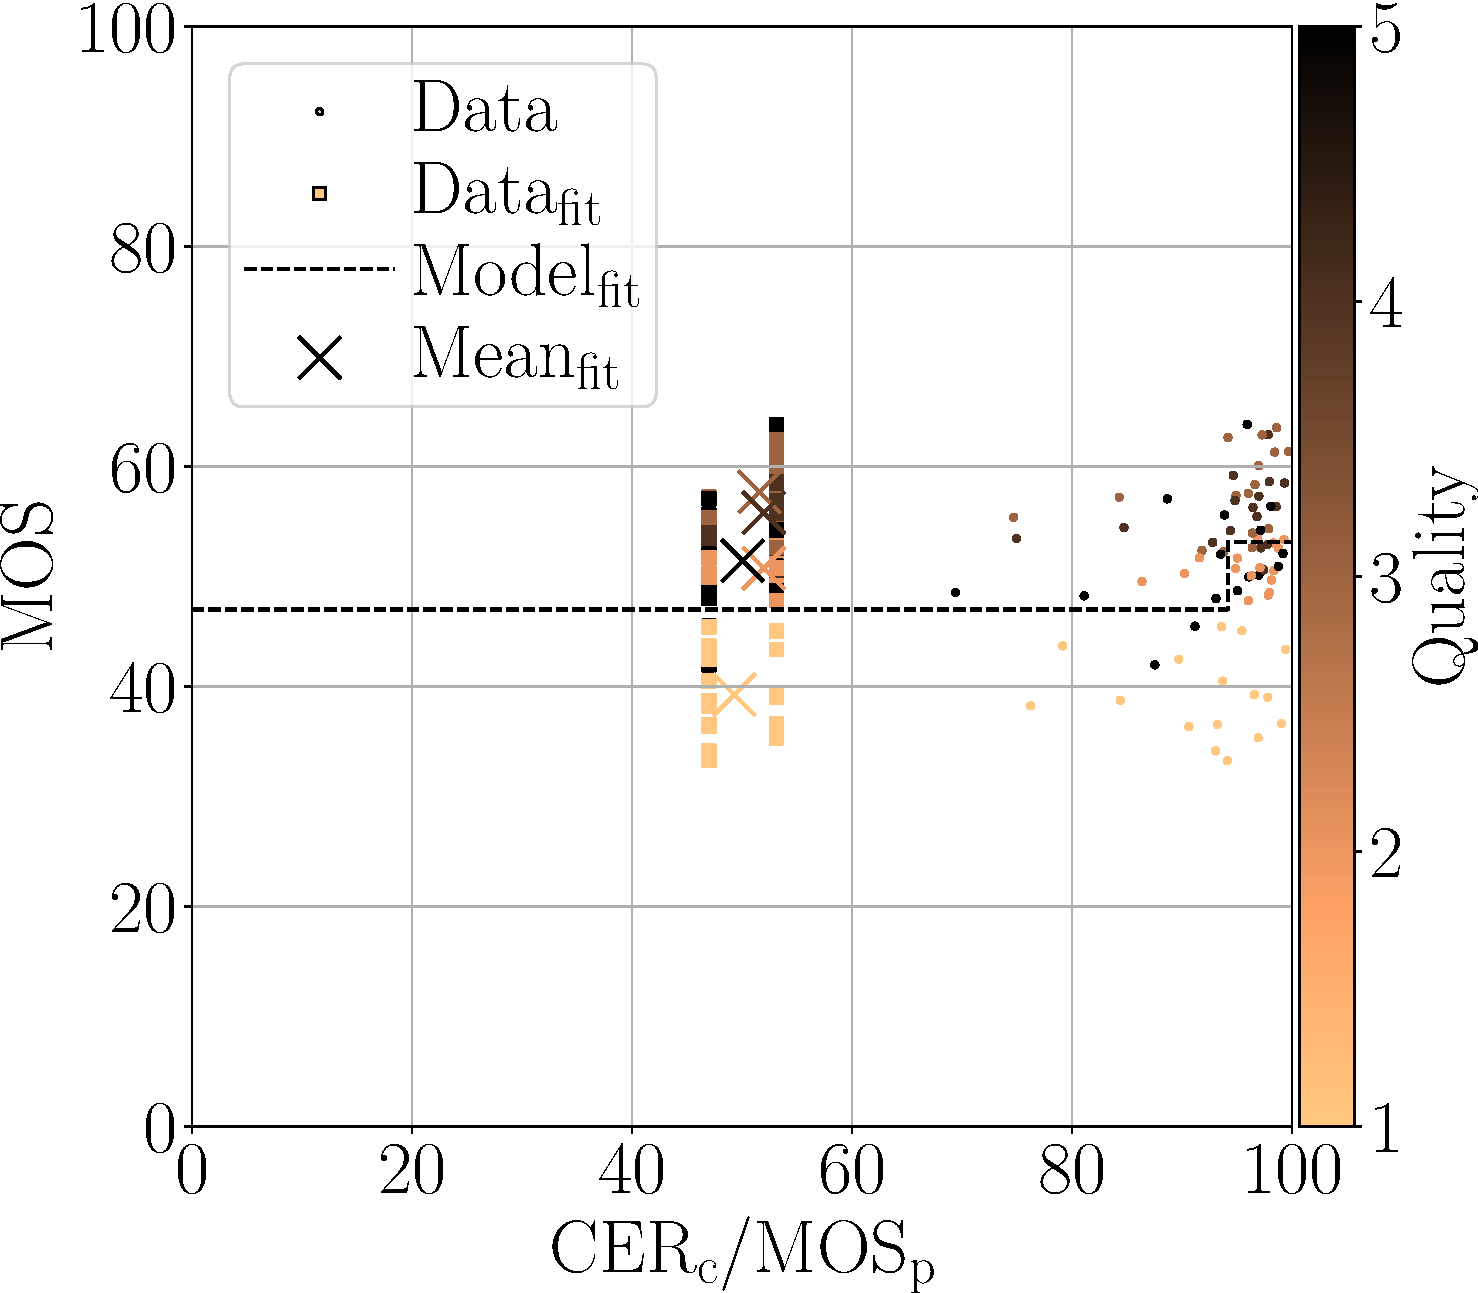
\includegraphics[width=\textwidth]{../../images/analyze/mos_cer_ref_fitted_mean_ezocr_CC.pdf}
        \caption{CC}
        \label{fig:mos_cer_ref_fitted_mean_ezocr_CC}
    \end{subfigure}%
    \hfill
    \begin{subfigure}[b]{0.32\textwidth}
        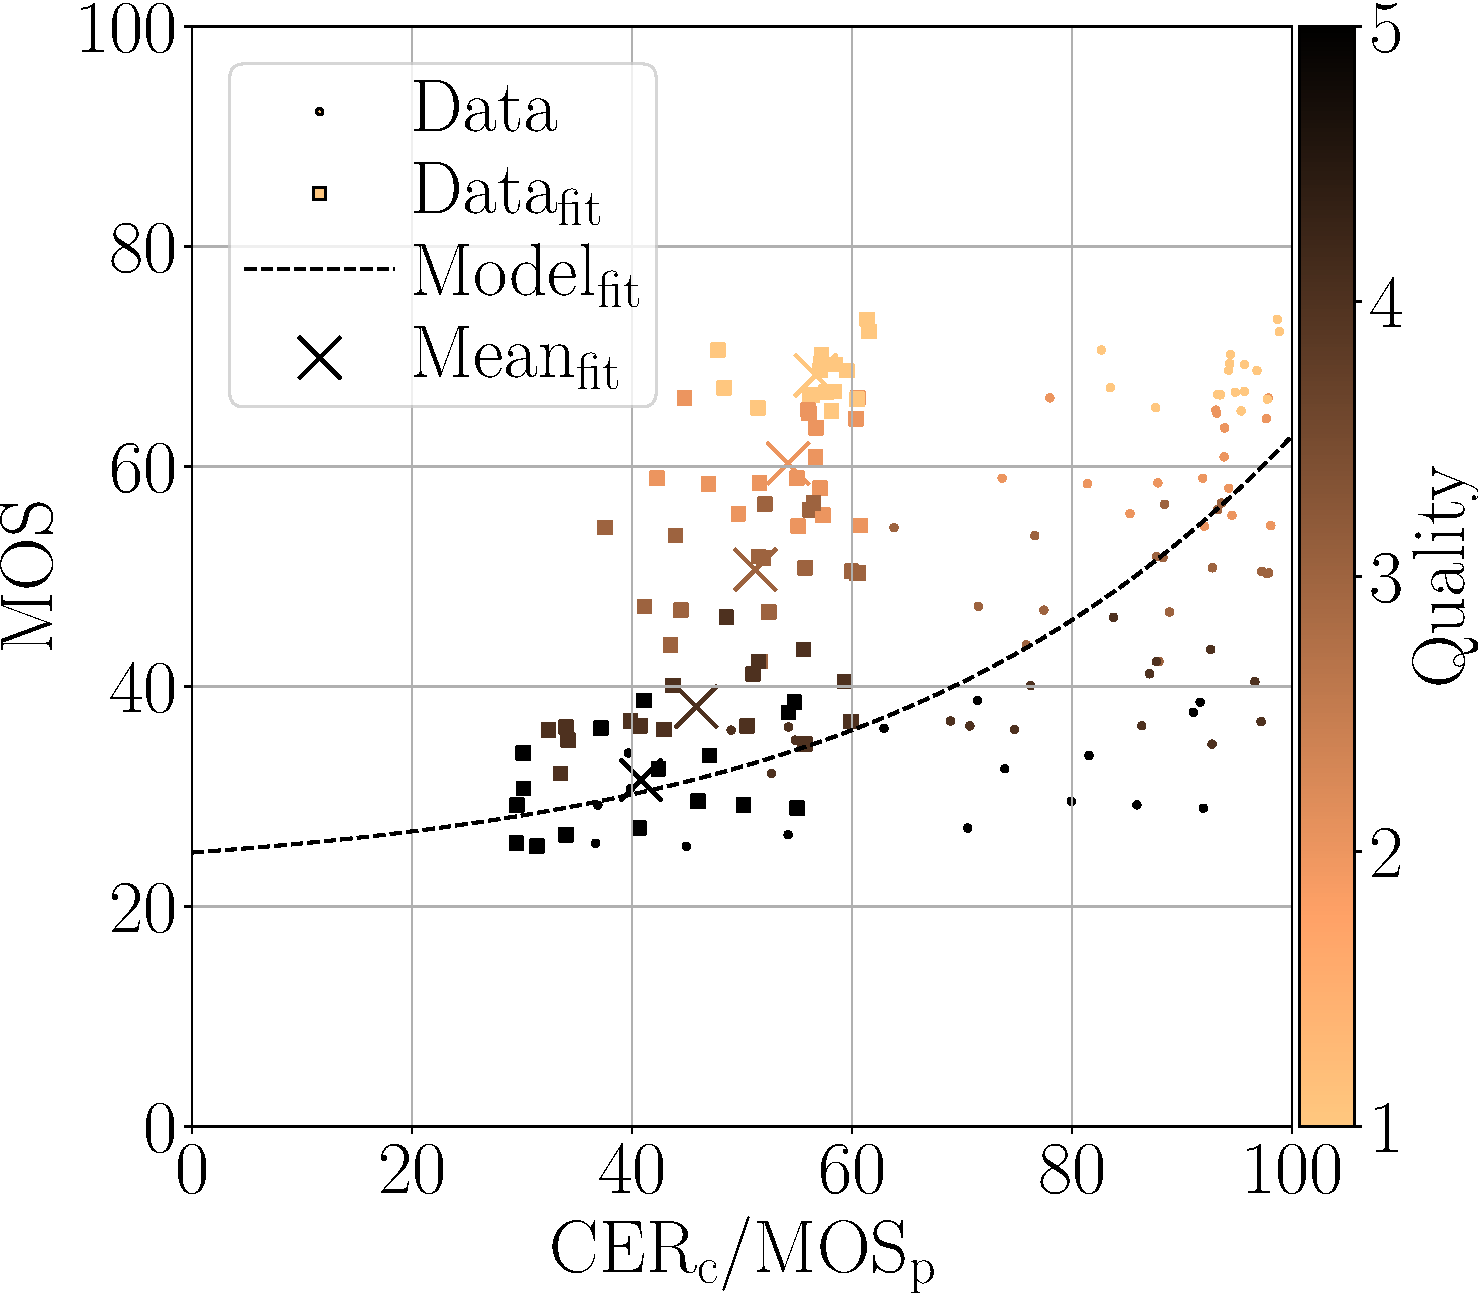
\includegraphics[width=\textwidth]{../../images/analyze/mos_cer_ref_fitted_mean_ezocr_JPEG.pdf}
        \caption{JPEG}
        \label{fig:mos_cer_ref_fitted_mean_ezocr_JPEG}
    \end{subfigure}%
    \hfill
    \begin{subfigure}[b]{0.32\textwidth}
        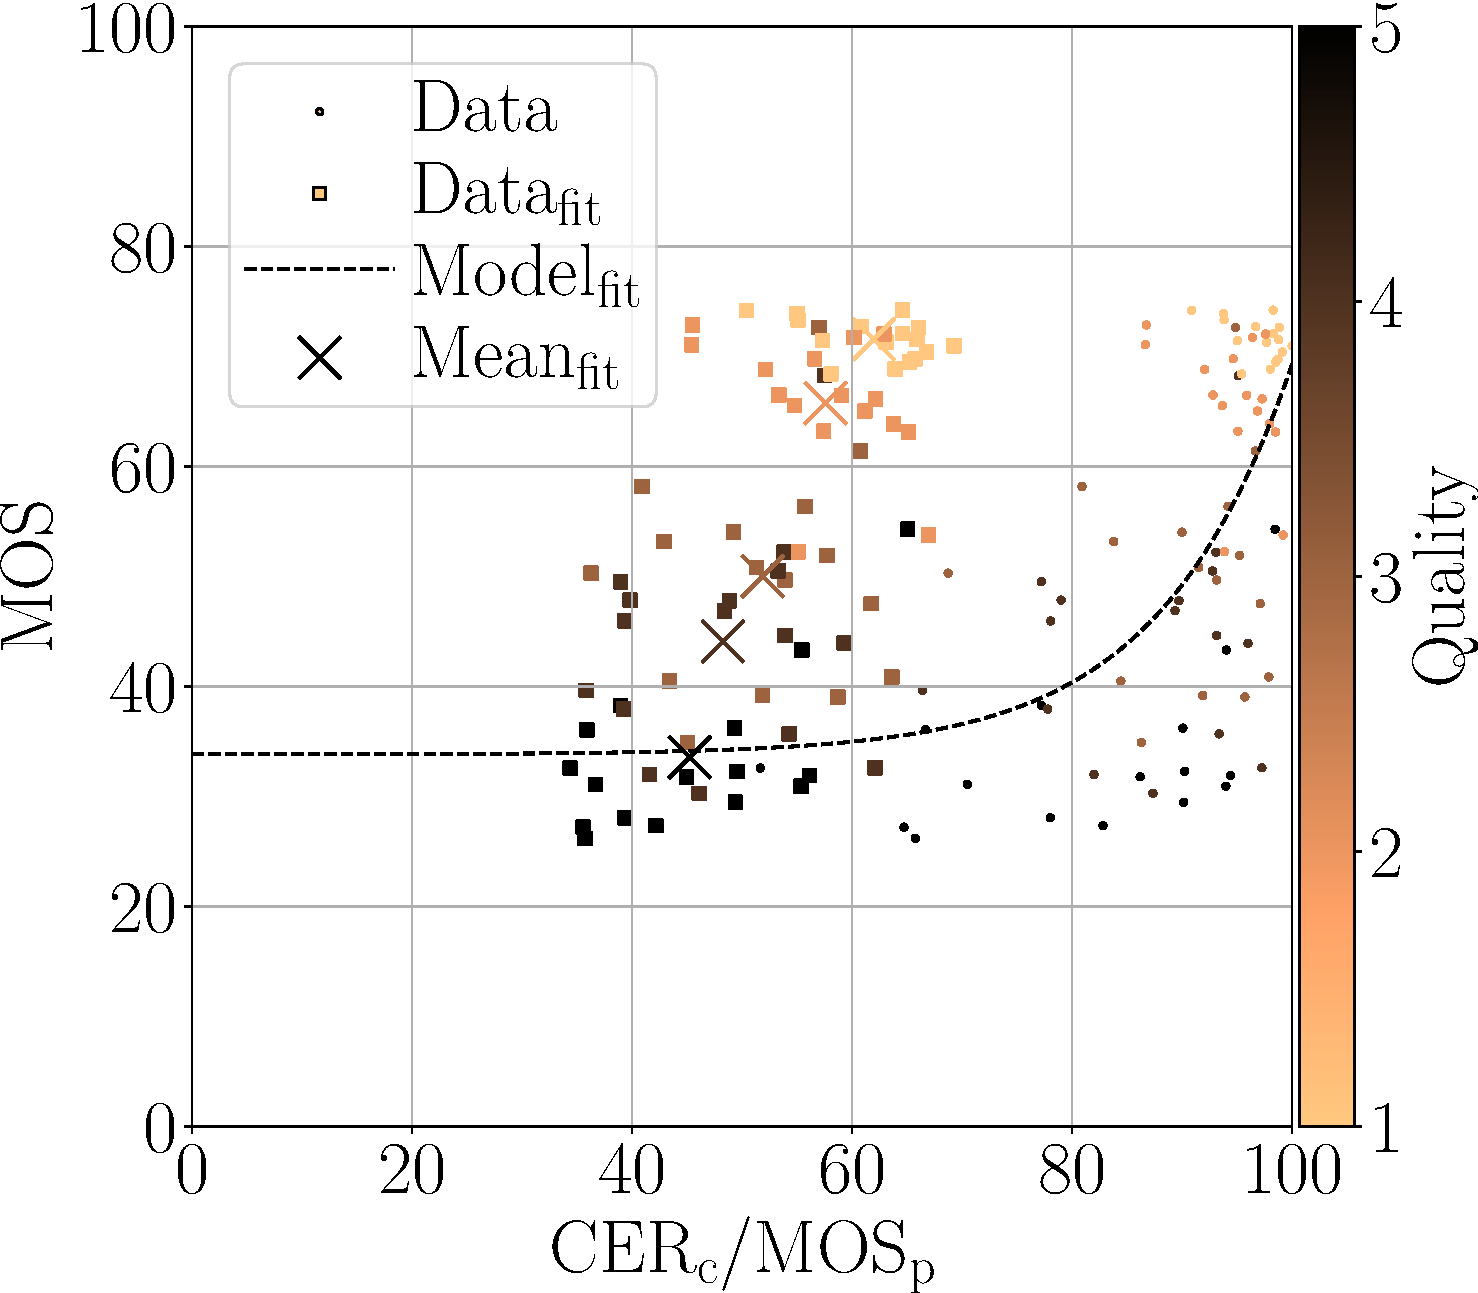
\includegraphics[width=\textwidth]{../../images/analyze/mos_cer_ref_fitted_mean_ezocr_JPEG2000.pdf}
        \caption{JPEG2000}
        \label{fig:mos_cer_ref_fitted_mean_ezocr_JPEG2000}
    \end{subfigure}%
    \newline
    \begin{subfigure}[b]{0.32\textwidth}
        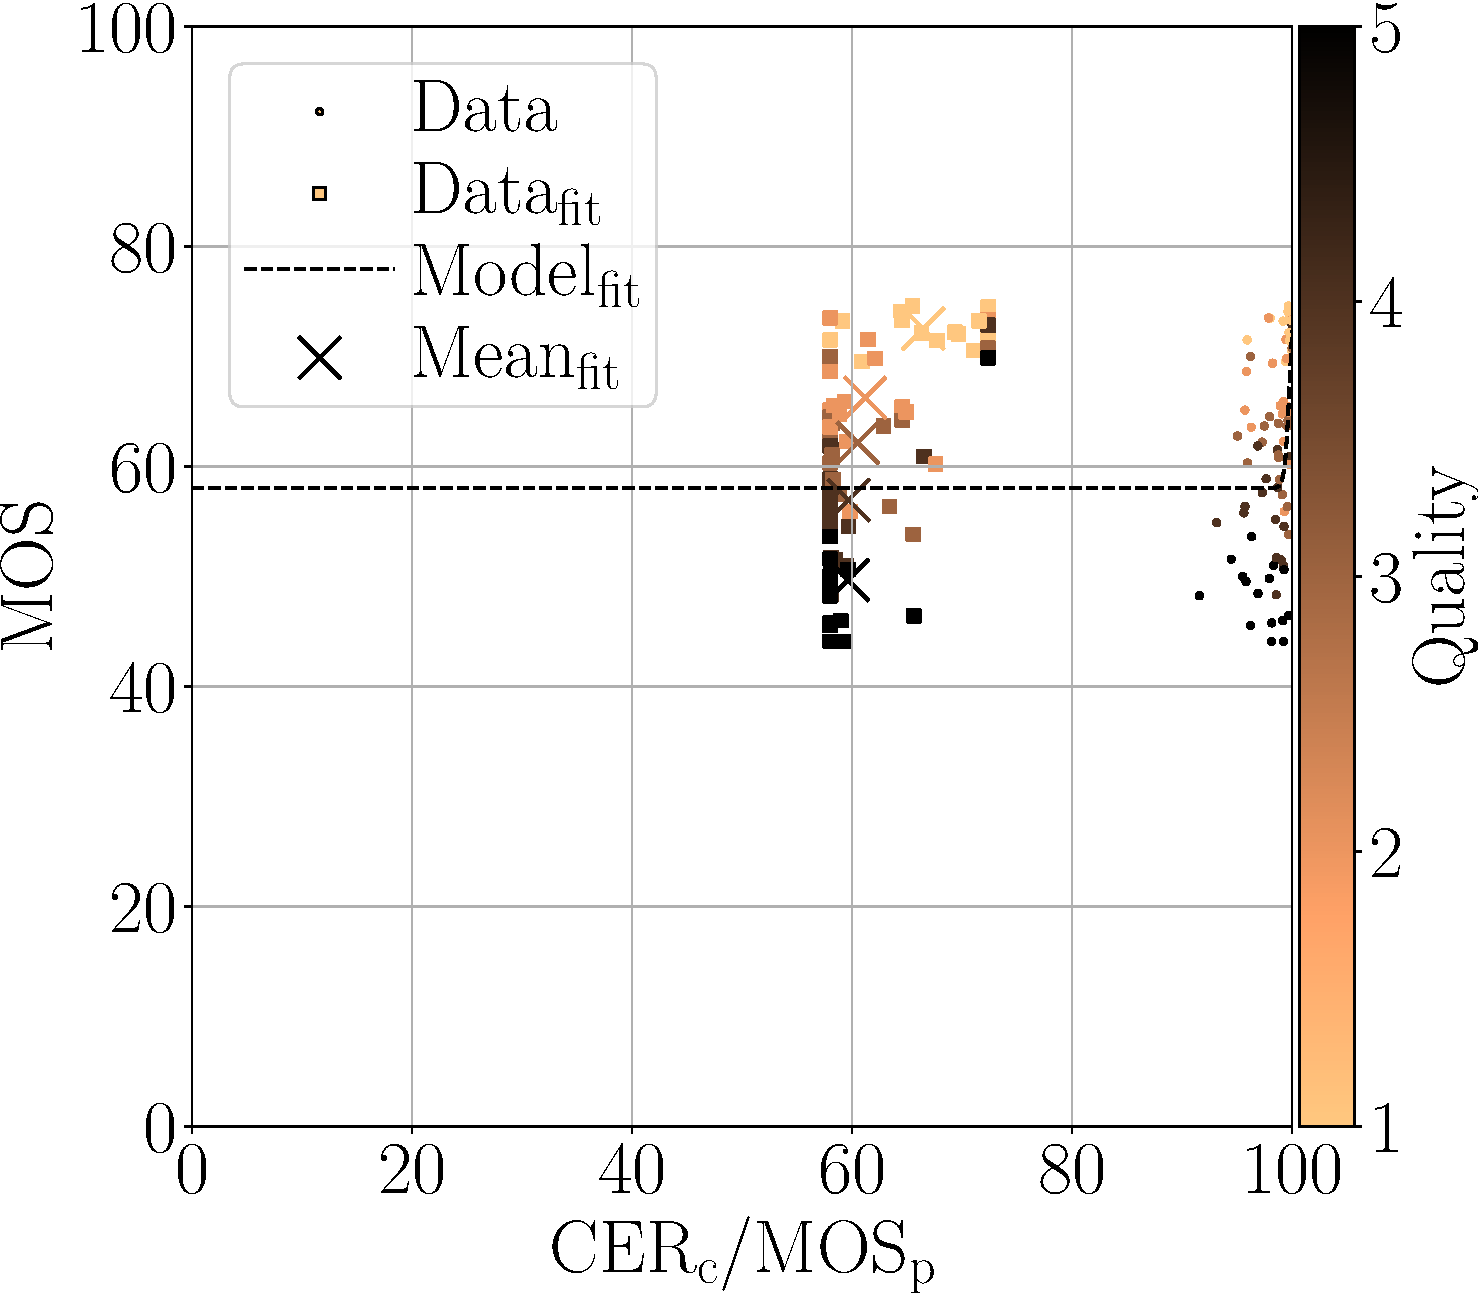
\includegraphics[width=\textwidth]{../../images/analyze/mos_cer_ref_fitted_mean_ezocr_CSC.pdf}
        \caption{CSC}
        \label{fig:mos_cer_ref_fitted_mean_ezocr_CSC}
    \end{subfigure}%
    \hfill
    \begin{subfigure}[b]{0.32\textwidth}
        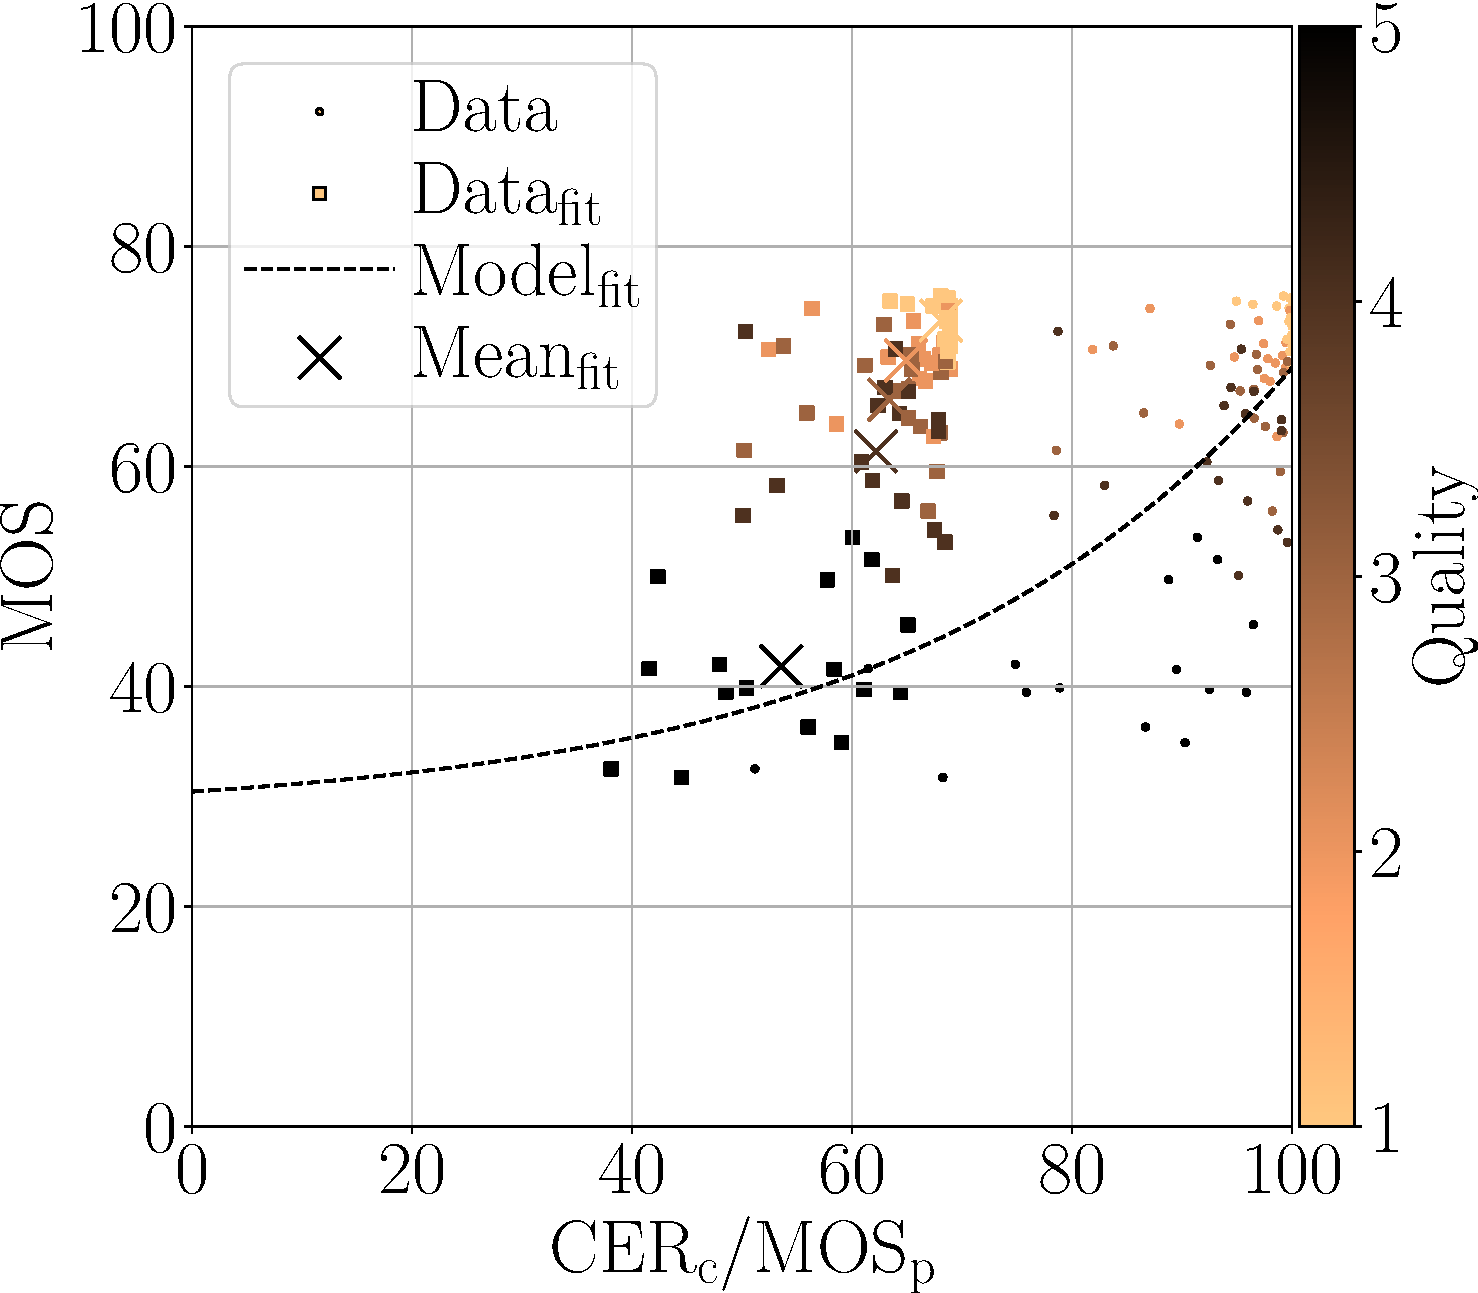
\includegraphics[width=\textwidth]{../../images/analyze/mos_cer_ref_fitted_mean_ezocr_HEVC-SCC.pdf}
        \caption{HEVC-SCC}
        \label{fig:mos_cer_ref_fitted_mean_ezocr_HEVC-SCC}
    \end{subfigure}%
    \hfill
    \begin{subfigure}[b]{0.32\textwidth}
        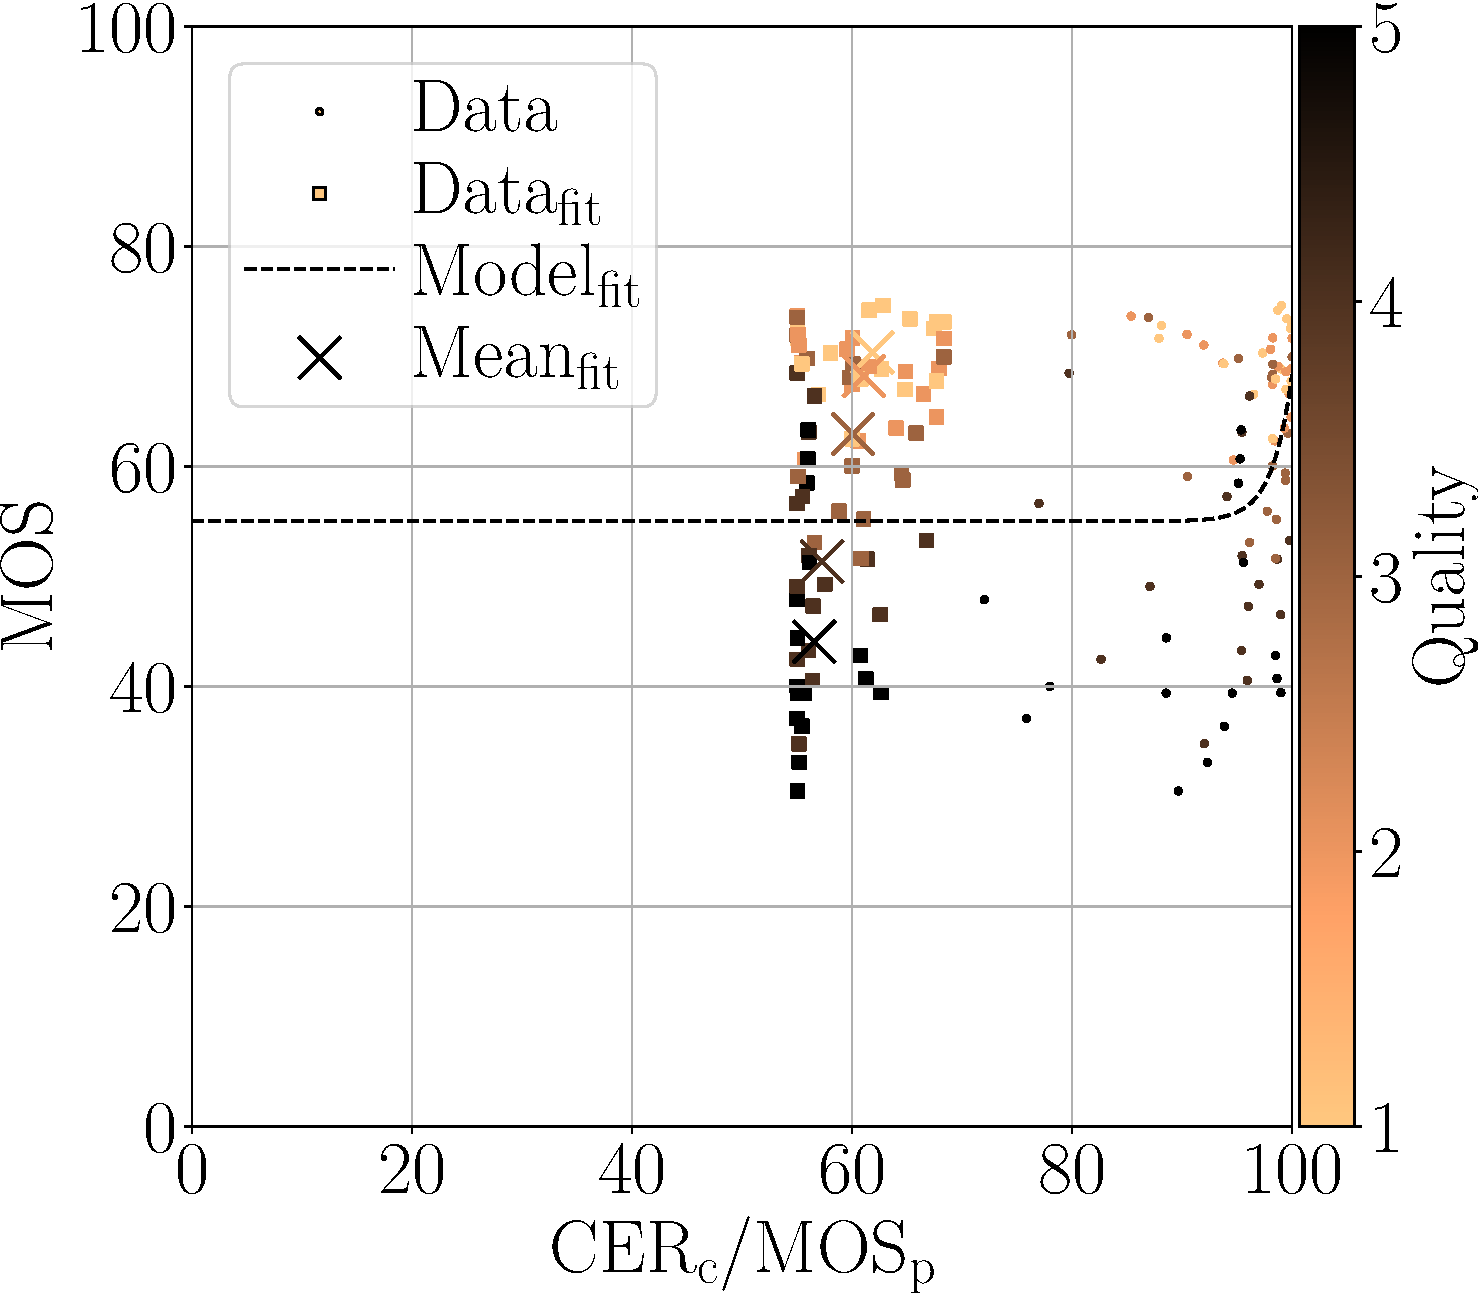
\includegraphics[width=\textwidth]{../../images/analyze/mos_cer_ref_fitted_mean_ezocr_CQD.pdf}
        \caption{CQD}
        \label{fig:mos_cer_ref_fitted_mean_ezocr_CQD}
    \end{subfigure}%
    \caption{Single datapoints ($\text{CER}_{\text{c}}$ vs \gls{mos}), the fitted model, the single datapoints after fitting ($\text{MOS}_{\text{p}}$ vs \gls{mos}) and the mean over each quality after fitting ($\text{MOS}_{\text{p}}$ vs \gls{mos}); all in relation to the text predictions on the reference images for different distortion types with EasyOCR.}
\label{fig:mos_cer_ref_fitted_mean_ezocr}
\end{figure}

In \autoref{fig:mos_cer_ref_fitted_mean_ezocr}, we can see the single $\text{CER}_{\text{c}}$ values plotted against the \gls{mos} for the selected images for all distortions with EasyOCR.
Additionally, we can see the model fitted to the datapoints.
Lastly, the resulting predicted \gls{mos} values $\text{MOS}_{\text{p}}$ and their mean over each quality are shown against the \gls{mos}.
The x-axis shows either the $\text{CER}_{\text{c}}$ or the modified values as $\text{MOS}_{\text{p}}$.
Firstly, we can observe that the models fit well to the data points and are monotonic.
The resulting $\text{MOS}_{\text{p}}$ values are generally moved to the center compared to the original $\text{CER}_{\text{c}}$ values.
This makes them have a more linear relationship to the \gls{mos} values.
For \gls{cc}, \gls{csc} and \gls{cqd} we can see that when the original points are very close to each other, it is difficult to fit a good model.
Thus, the resulting $\text{MOS}_{\text{p}}$ values seem to be almost constant, which is undesirable as they lose their predictive value, because the \gls{mos} values are obviously not constant.
As we mentioned before, this is expected due to the superior performance of EasyOCR on these distortions for all quality levels.

% We did this to reduce nonlinearities in the objective values and to generally conform to the evaluation methods of other literature in the field.


% mos vs cer (fitted) mean in relation to reference for Tesseract
\begin{figure}[h!]
\centering
    \begin{subfigure}[b]{0.32\textwidth}
        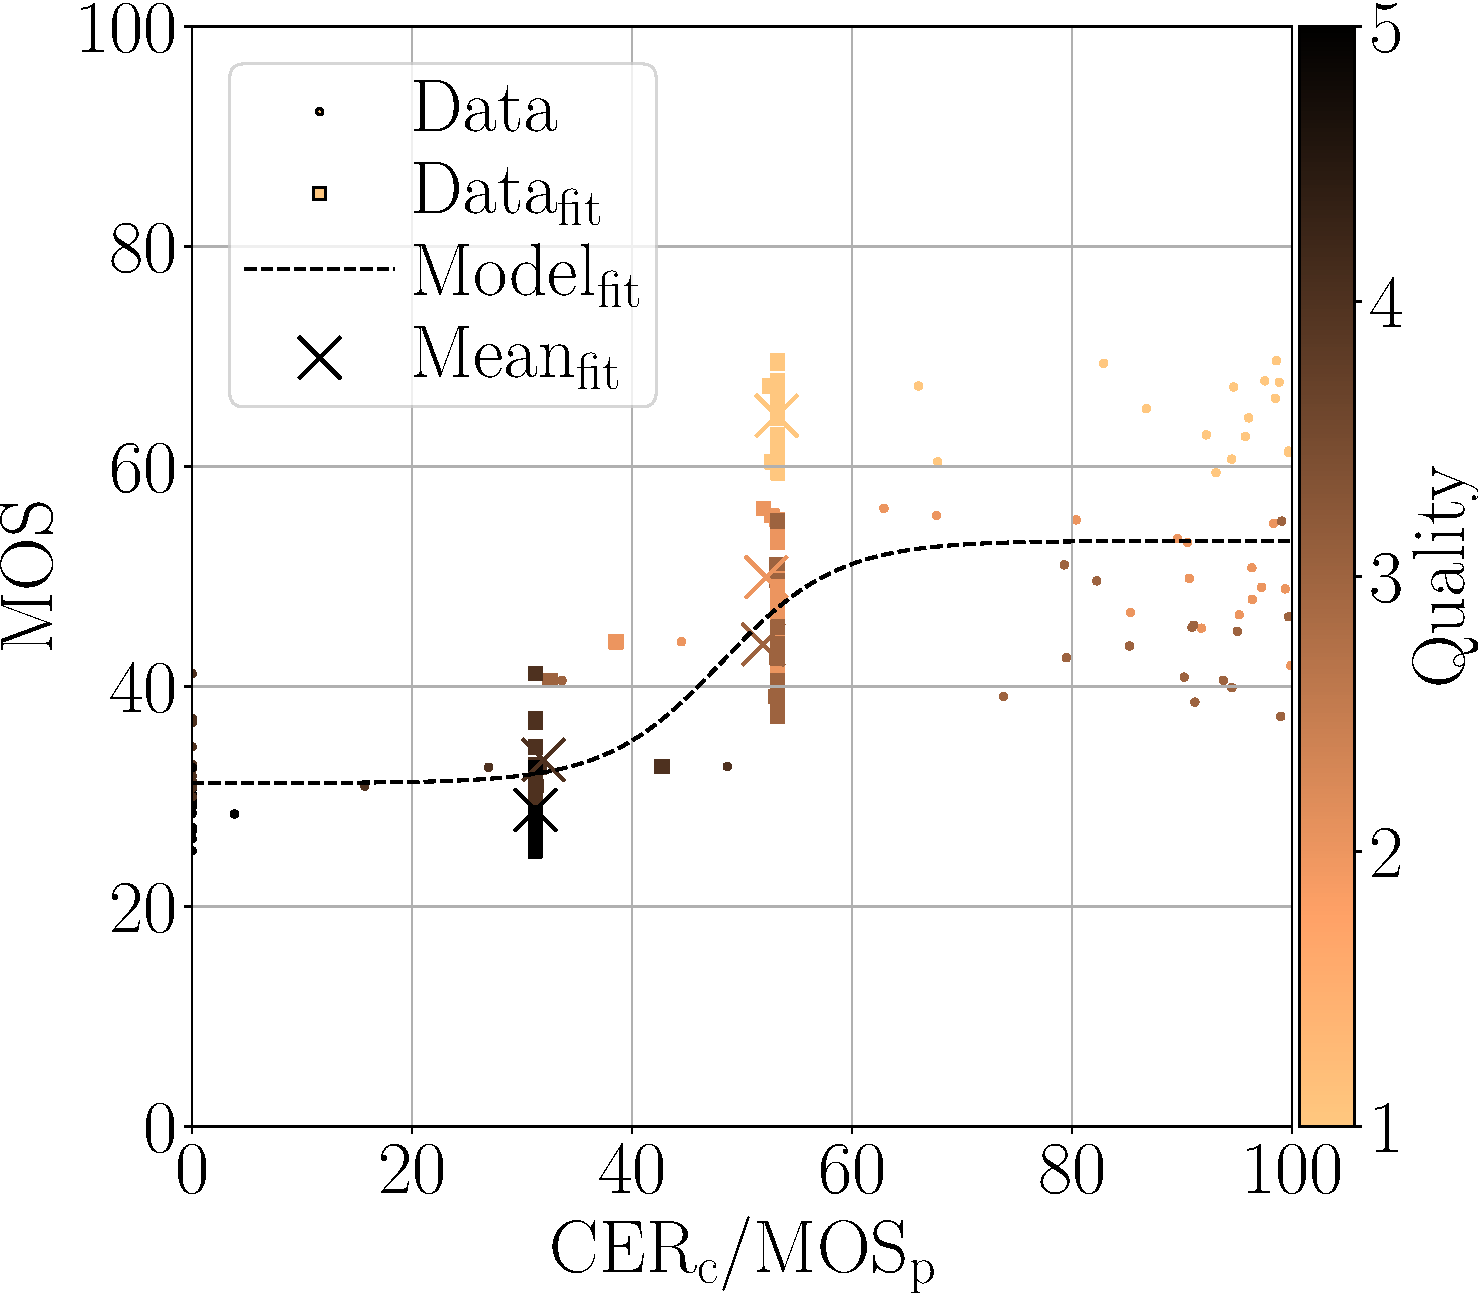
\includegraphics[width=\textwidth]{../../images/analyze/mos_cer_ref_fitted_mean_tess_GN.pdf}
        \caption{GN}
        \label{fig:mos_cer_ref_fitted_mean_tess_GN}
    \end{subfigure}%
    \hfill
    \begin{subfigure}[b]{0.32\textwidth}
        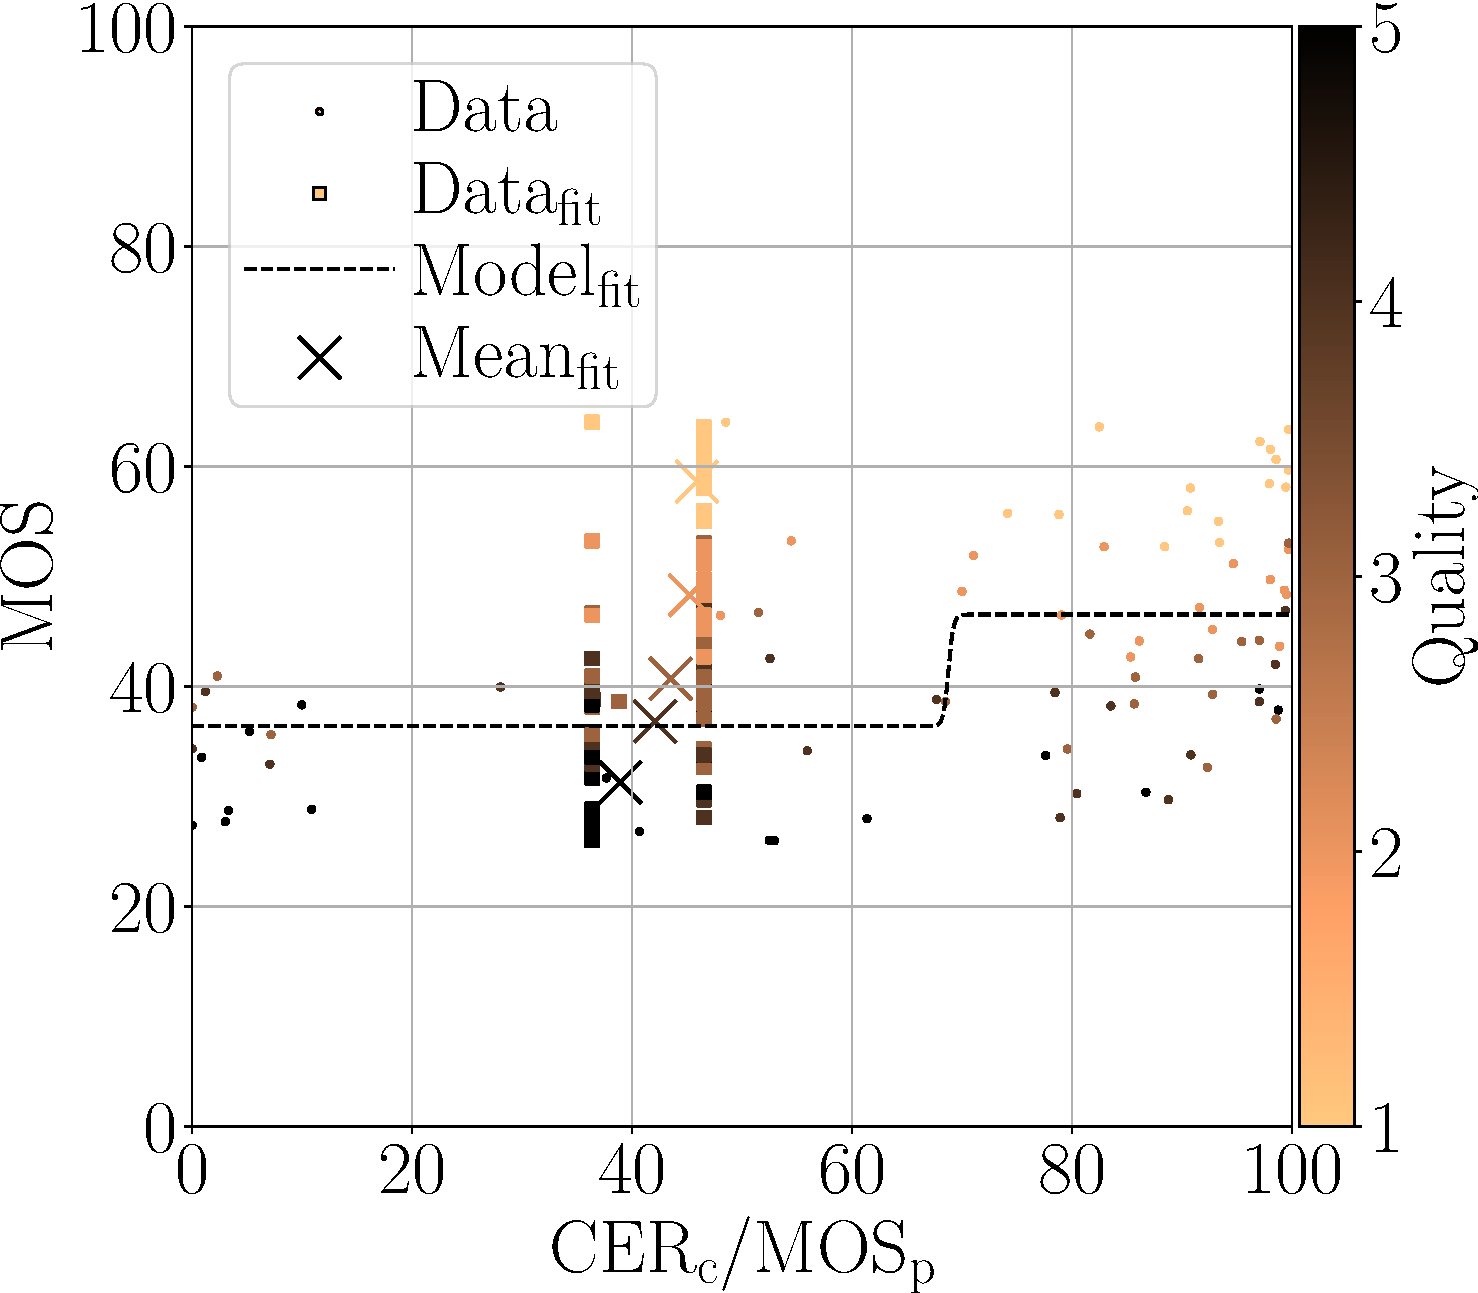
\includegraphics[width=\textwidth]{../../images/analyze/mos_cer_ref_fitted_mean_tess_GB.pdf}
        \caption{GB}
        \label{fig:mos_cer_ref_fitted_mean_tess_GB}
    \end{subfigure}%
    \hfill
    \begin{subfigure}[b]{0.32\textwidth}
        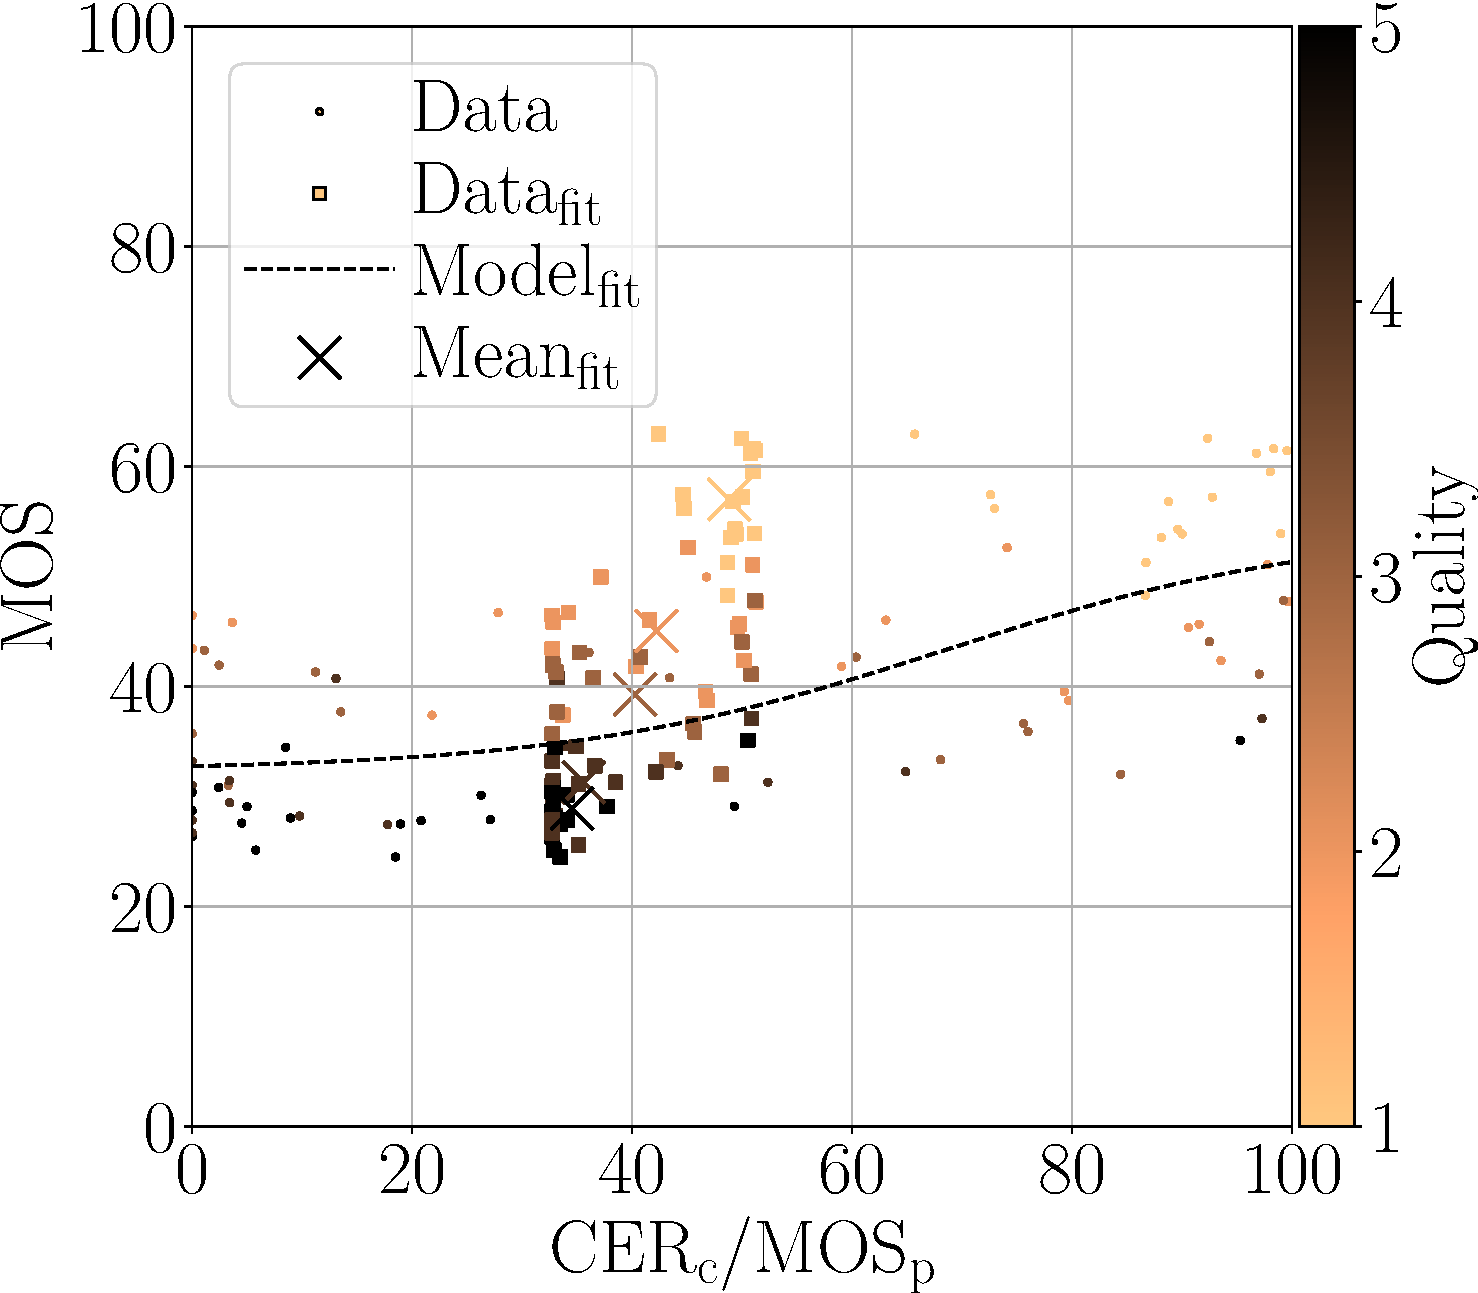
\includegraphics[width=\textwidth]{../../images/analyze/mos_cer_ref_fitted_mean_tess_MB.pdf}
        \caption{MB}
        \label{fig:mos_cer_ref_fitted_mean_tess_MB}
    \end{subfigure}%
    \newline
    \begin{subfigure}[b]{0.32\textwidth}
        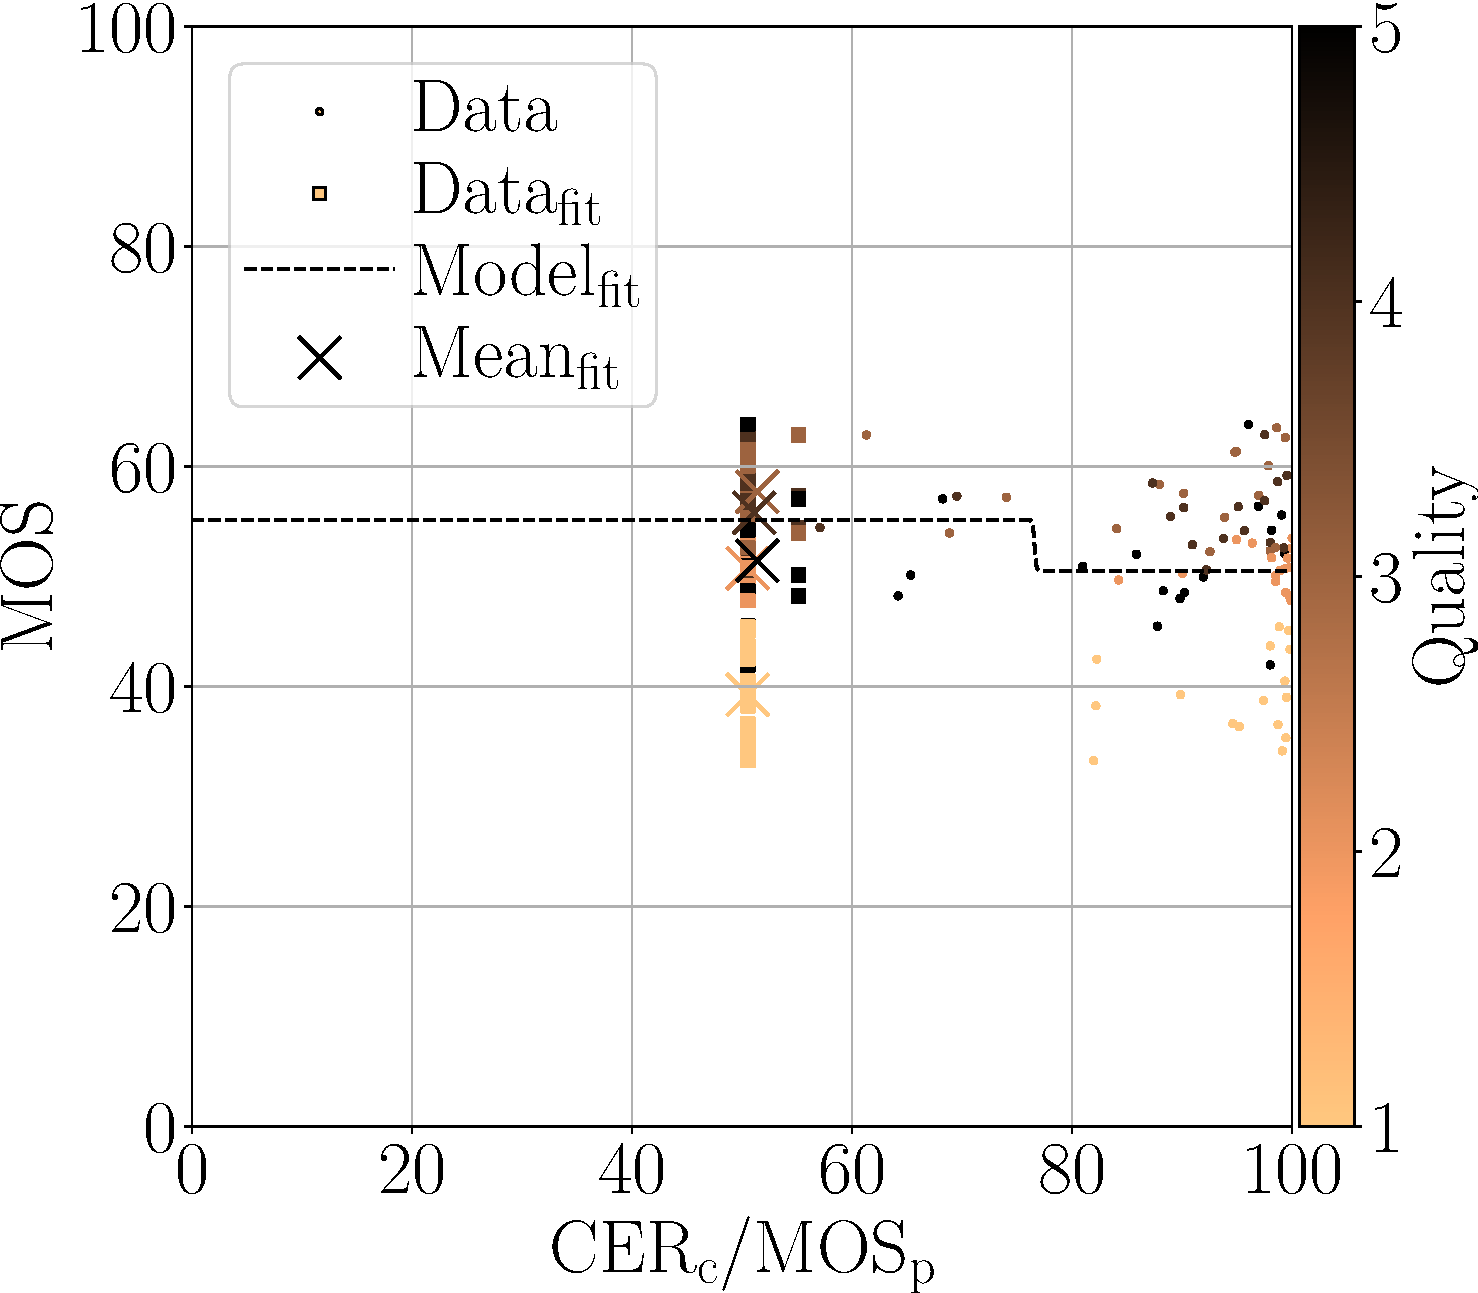
\includegraphics[width=\textwidth]{../../images/analyze/mos_cer_ref_fitted_mean_tess_CC.pdf}
        \caption{CC}
        \label{fig:mos_cer_ref_fitted_mean_tess_CC}
    \end{subfigure}%
    \hfill
    \begin{subfigure}[b]{0.32\textwidth}
        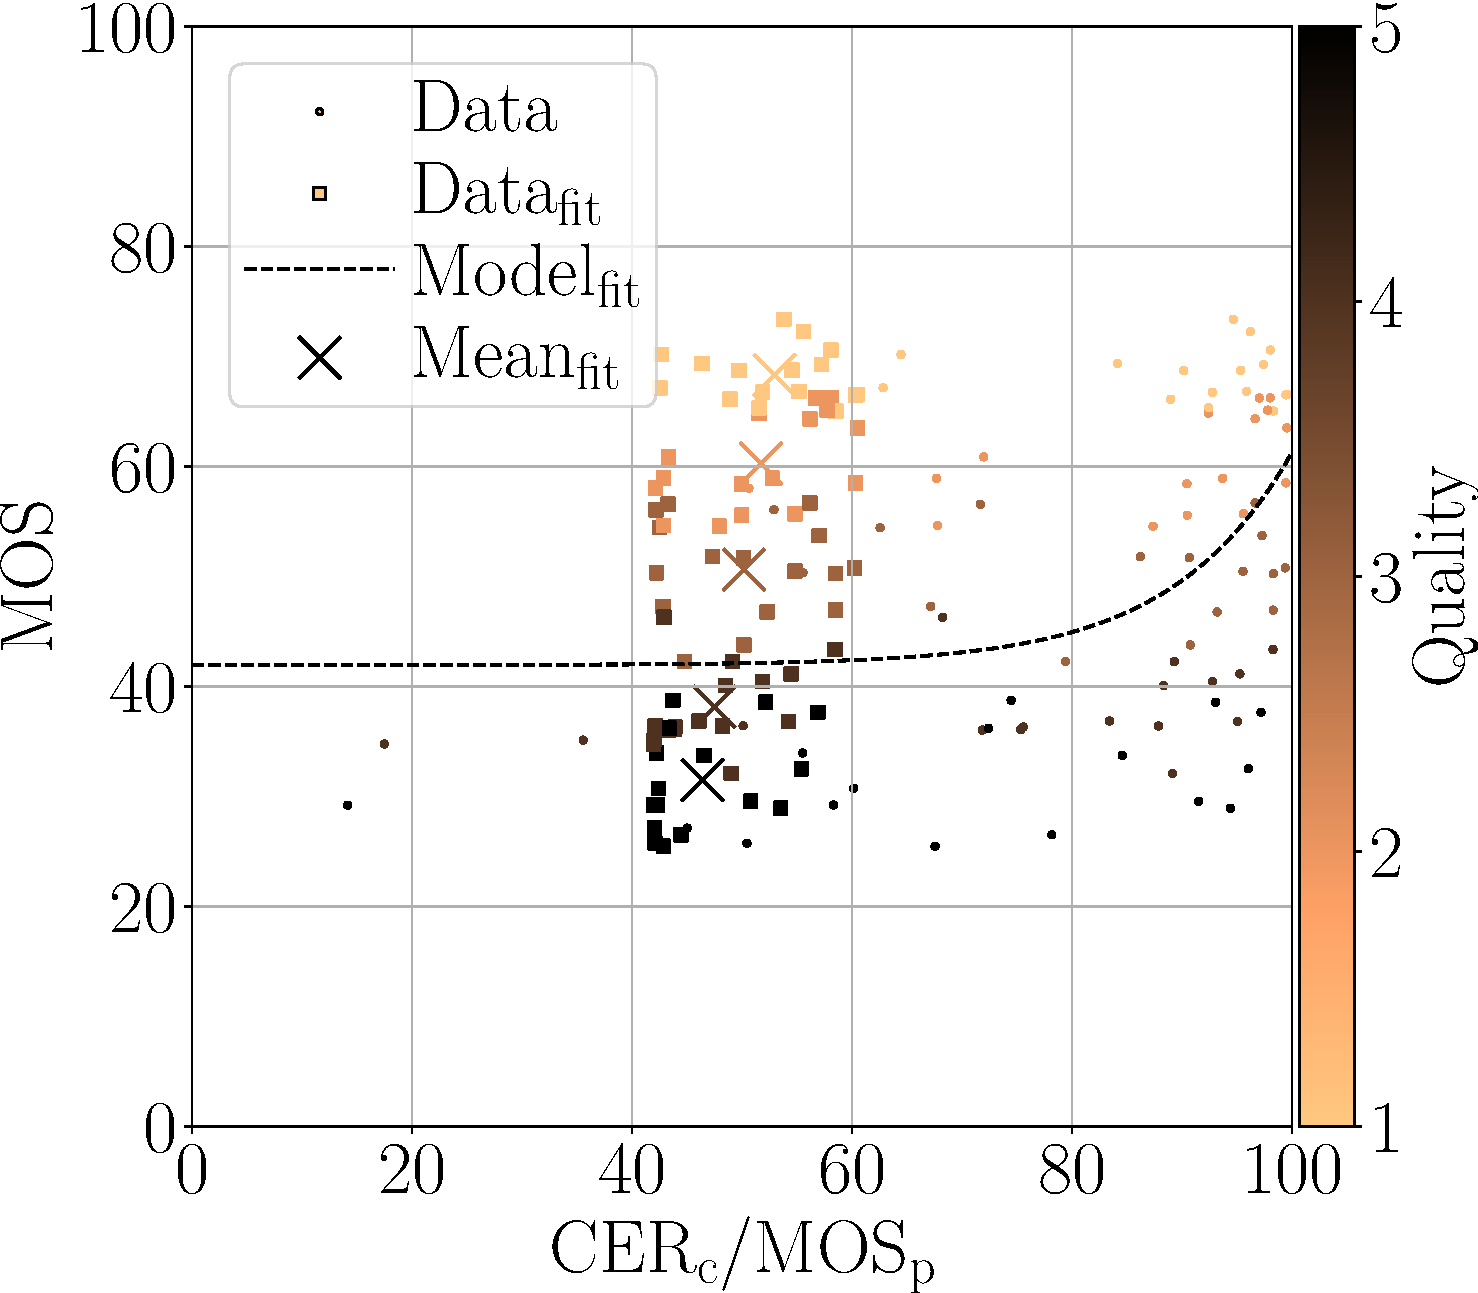
\includegraphics[width=\textwidth]{../../images/analyze/mos_cer_ref_fitted_mean_tess_JPEG.pdf}
        \caption{JPEG}
        \label{fig:mos_cer_ref_fitted_mean_tess_JPEG}
    \end{subfigure}%
    \hfill
    \begin{subfigure}[b]{0.32\textwidth}
        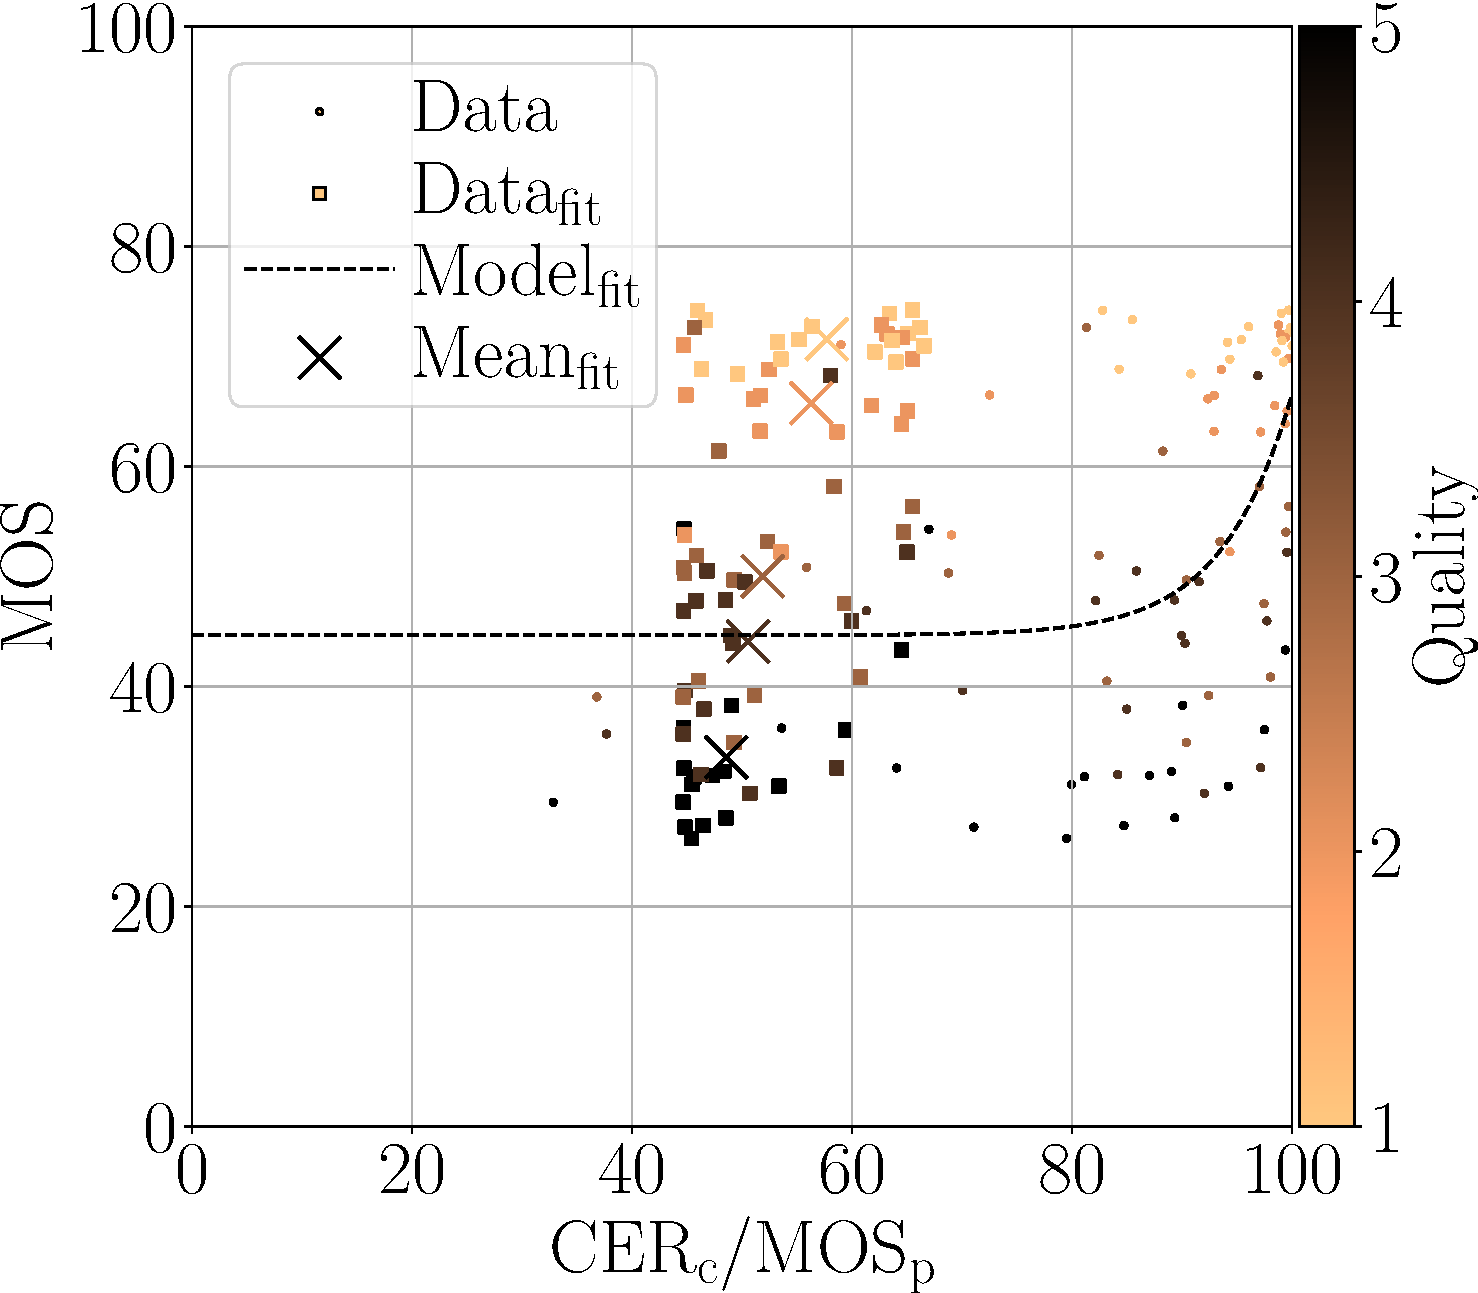
\includegraphics[width=\textwidth]{../../images/analyze/mos_cer_ref_fitted_mean_tess_JPEG2000.pdf}
        \caption{JPEG2000}
        \label{fig:mos_cer_ref_fitted_mean_tess_JPEG2000}
    \end{subfigure}%
    \newline
    \begin{subfigure}[b]{0.32\textwidth}
        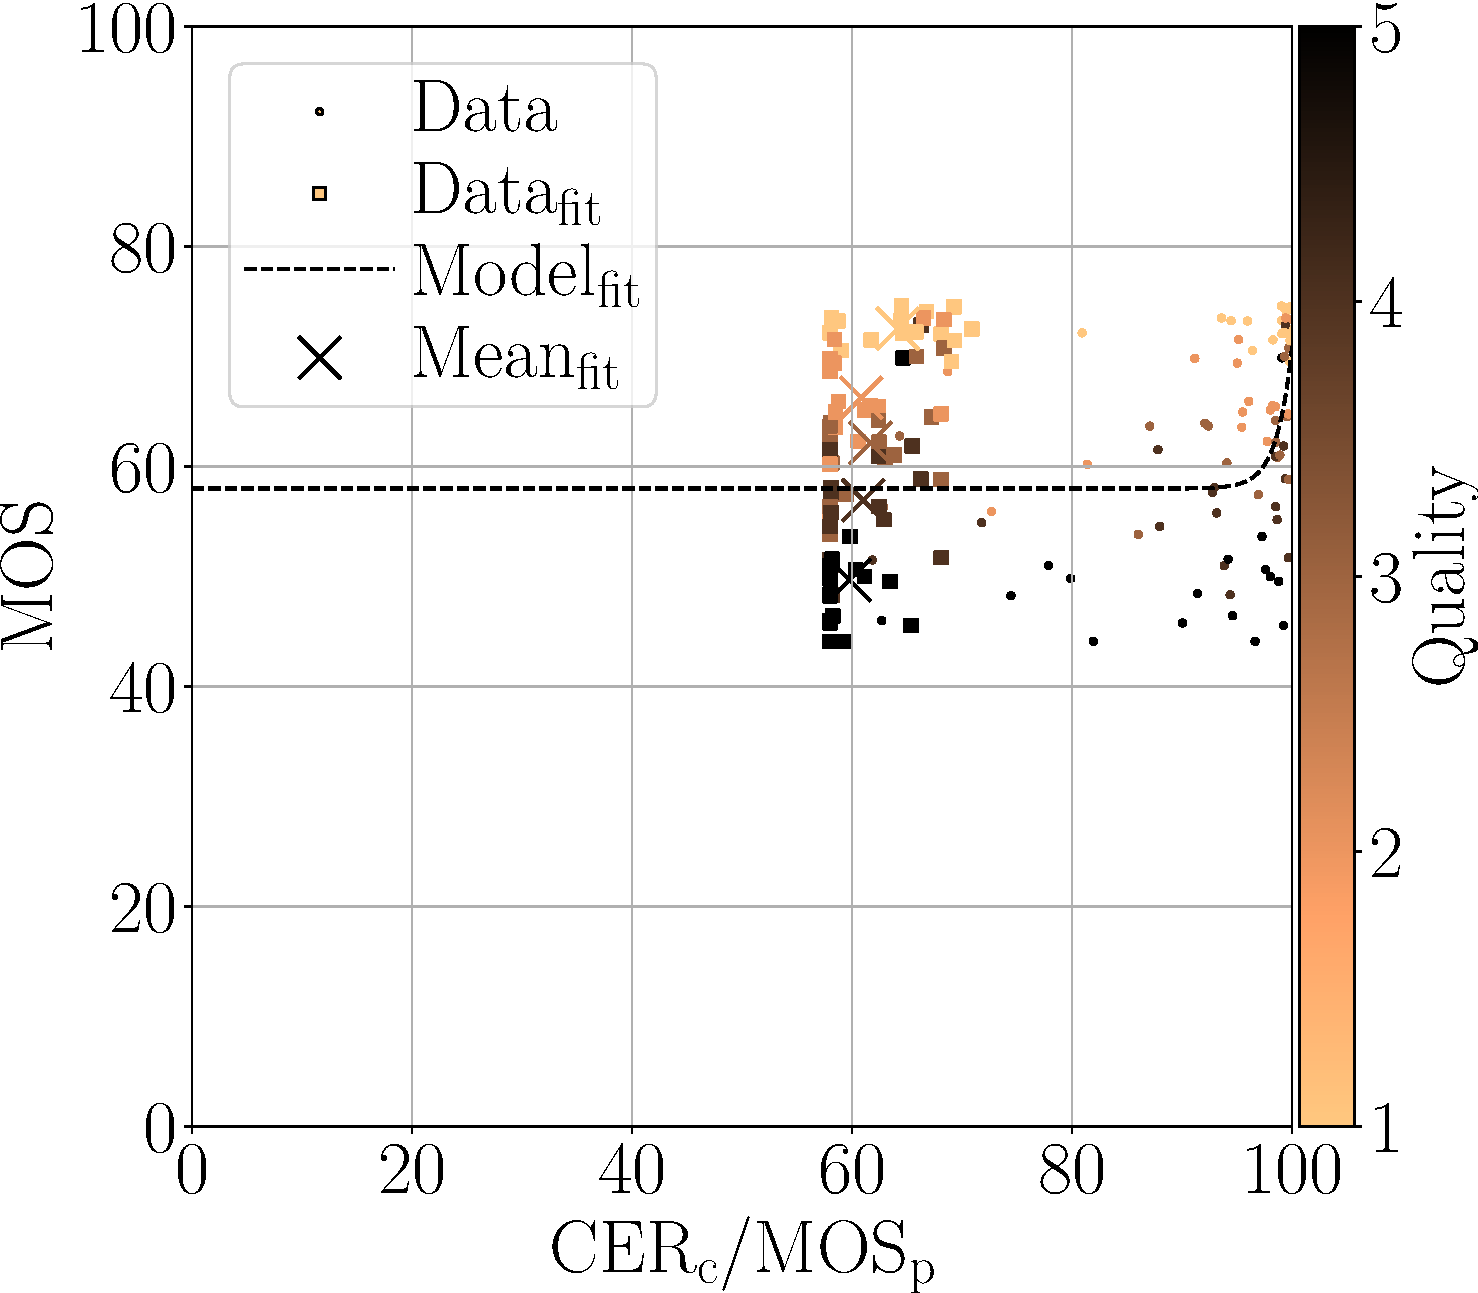
\includegraphics[width=\textwidth]{../../images/analyze/mos_cer_ref_fitted_mean_tess_CSC.pdf}
        \caption{CSC}
        \label{fig:mos_cer_ref_fitted_mean_tess_CSC}
    \end{subfigure}%
    \hfill
    \begin{subfigure}[b]{0.32\textwidth}
        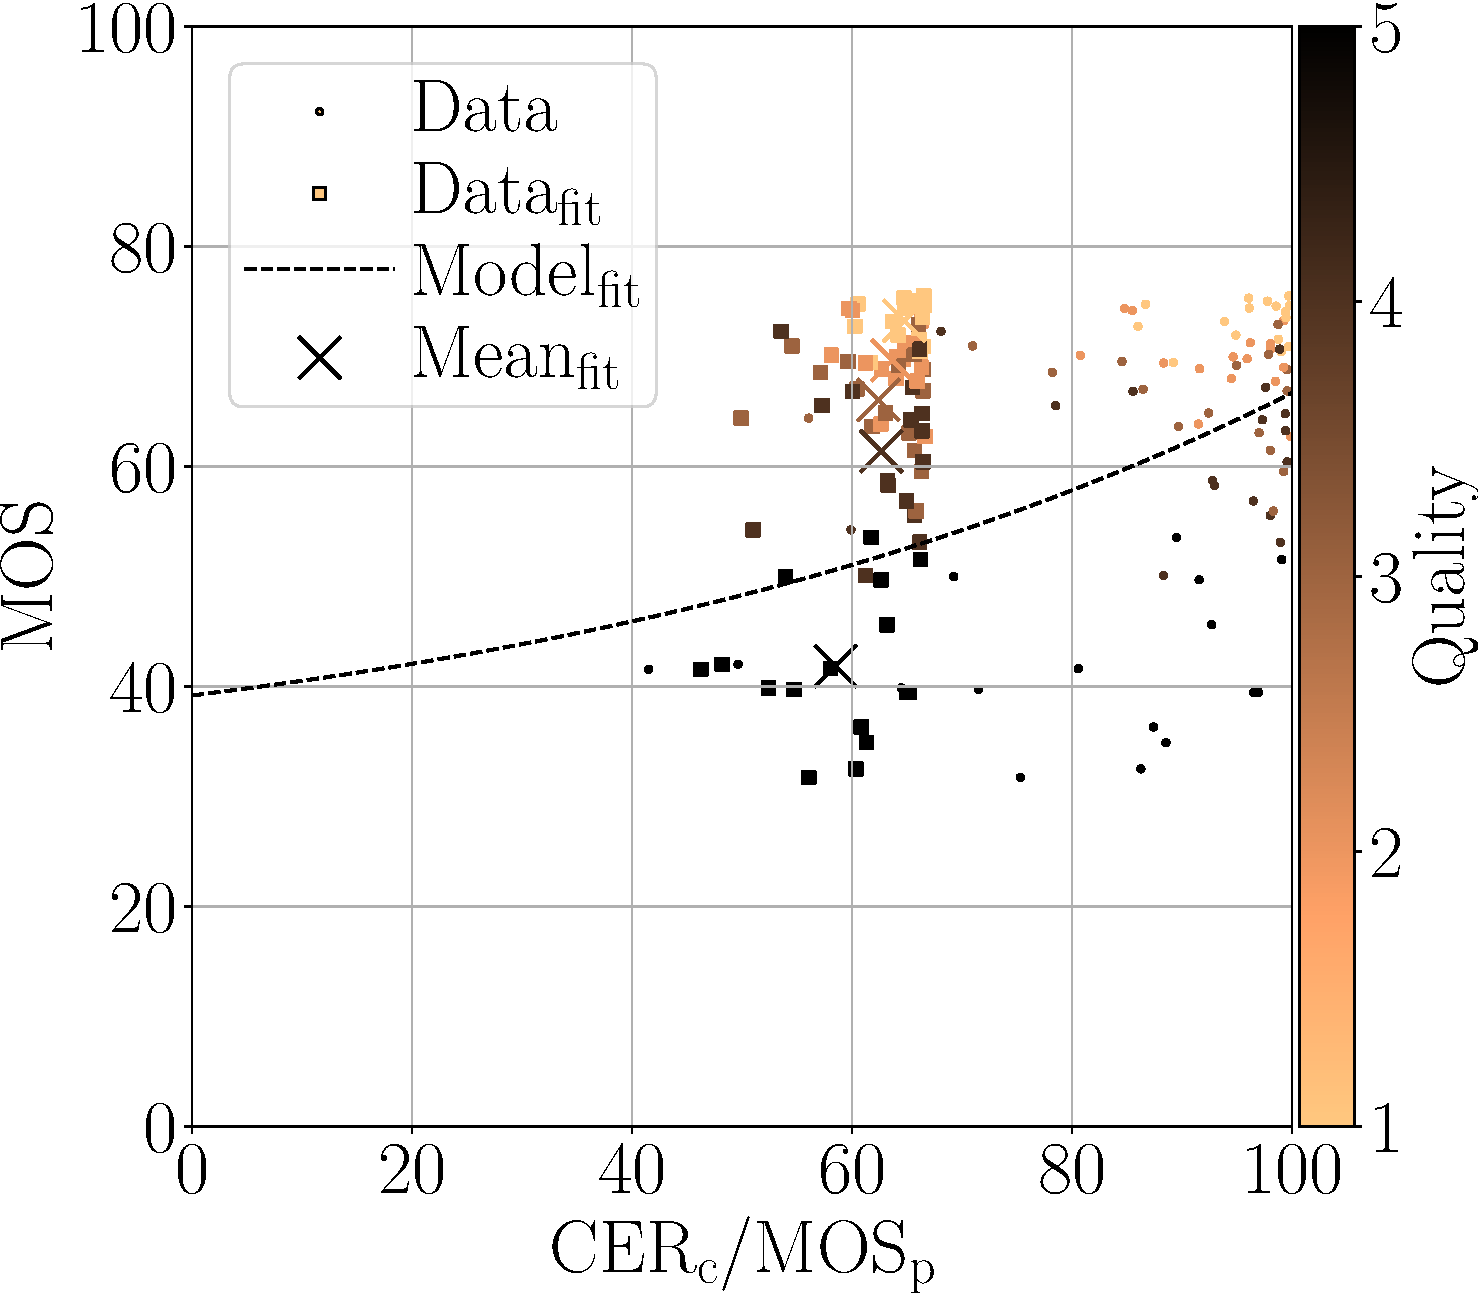
\includegraphics[width=\textwidth]{../../images/analyze/mos_cer_ref_fitted_mean_tess_HEVC-SCC.pdf}
        \caption{HEVC-SCC}
        \label{fig:mos_cer_ref_fitted_mean_tess_HEVC-SCC}
    \end{subfigure}%
    \hfill
    \begin{subfigure}[b]{0.32\textwidth}
        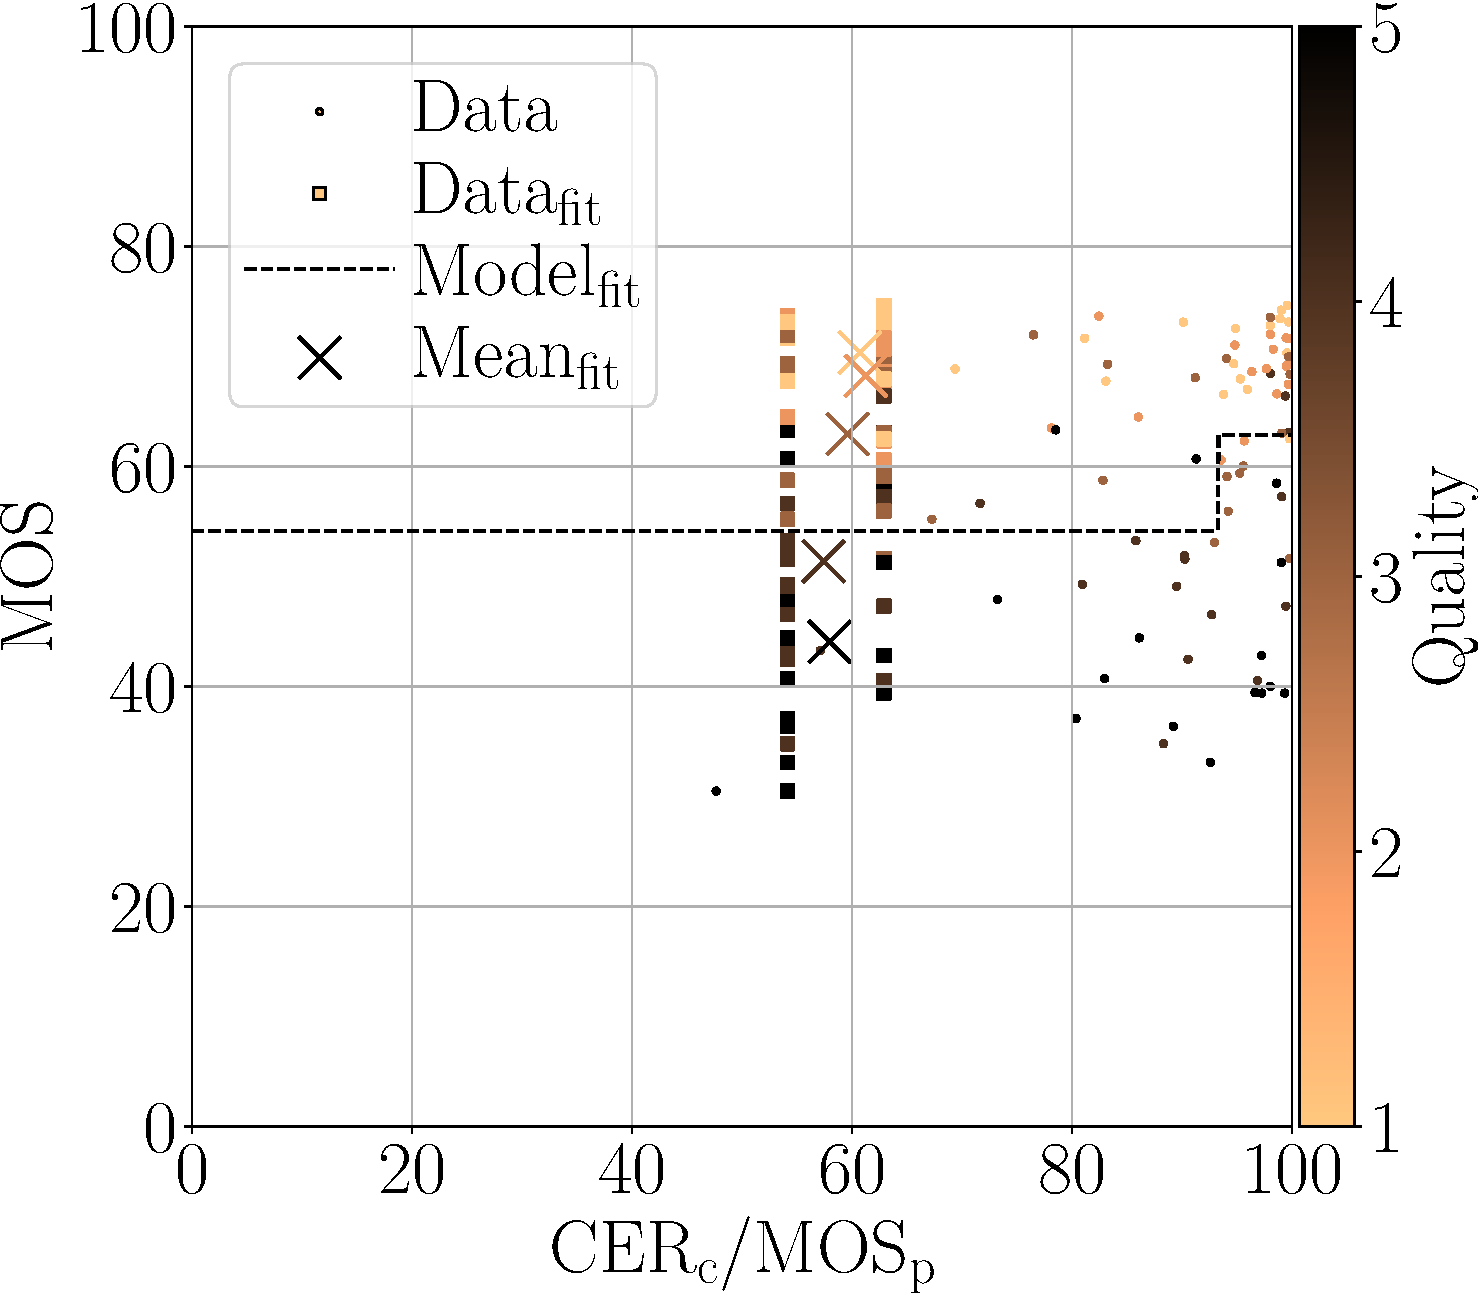
\includegraphics[width=\textwidth]{../../images/analyze/mos_cer_ref_fitted_mean_tess_CQD.pdf}
        \caption{CQD}
        \label{fig:mos_cer_ref_fitted_mean_tess_CQD}
    \end{subfigure}%
    \caption{Single datapoints ($\text{CER}_{\text{c}}$ vs \gls{mos}), the fitted model, the single datapoints after fitting ($\text{MOS}_{\text{p}}$ vs \gls{mos}) and the mean over each quality after fitting ($\text{MOS}_{\text{p}}$ vs \gls{mos}); all in relation to the text predictions on the reference images for different distortion types with Tesseract \gls{ocr}.}
\label{fig:mos_cer_ref_fitted_mean_tess}
\end{figure}

We do the same for Tesseract in \autoref{fig:mos_cer_ref_fitted_mean_tess}.
Compared to the fitting for EasyOCR, it is difficult to see any meaningful differences.
One noticeable difference is, that curves for \gls{gn} and \gls{gb} now also produce relatively constant $\text{MOS}_{\text{p}}$ values.
However to quantify and compare our results, we will look at correlations and the \gls{rmse} in the next part.

\begin{table}[h!]
    \centering
    \begin{tabular}{|l|rrr|}
        \hline
        Distortion Type & SRCC & PLCC & RMSE \\
        \hline
        \hline
        CC & 0.29 & 0.40 & 6.76 \\
        CQD & 0.28 & 0.36 & 11.45 \\
        CSC & 0.47 & 0.54 & 7.65 \\
        GB & \textbf{0.70} & \textbf{0.71} & 7.40 \\
        GN & 0.56 & 0.54 & 11.09 \\
        HEVC-SCC & 0.57 & 0.62 & 9.42 \\
        JPEG & 0.65 & 0.66 & 10.65 \\
        JPEG2000 & 0.59 & 0.61 & 12.41 \\
        MB & \textbf{0.86} & \textbf{0.85} & \textbf{5.73} \\
        \hline
        Overall & 0.65 & 0.66 & 9.44 \\
        \hline
    \end{tabular}
    \caption{\gls{srcc} between $\text{CER}_{\text{c}}$ and \gls{mos}; \gls{plcc} and \gls{rmse} between $\text{MOS}_{\text{p}}$ and \gls{mos} for different distortion types and for all distortions together (overall) for EasyOCR.}
    \label{tab:fitted_metrics_ezocr}
\end{table}

To quantify the observations we calculate the \gls{srcc} (prediction monotonicity), \gls{plcc} (prediction consistency) and \gls{rmse} (prediction accuracy) as described in \autoref{chap:qualityassessment}.
In \autoref{tab:fitted_metrics_ezocr}, we can see metrics for each distortion separately and for all distortions together (overall) for EasyOCR.

Most noteworthy are the results for \gls{mb}.
It shows the highest \gls{srcc} and \gls{plcc} and the lowest \gls{rmse}.
This means that the predicted $\text{MOS}_{\text{p}}$ values are a decent approximation of the \gls{mos} values.
Second, the \gls{gb} distortion shows the second highest \gls{srcc} and \gls{plcc} and the second lowest \gls{rmse}.
However, it is 15 points below the \gls{mb} distortion in \gls{srcc} and \gls{plcc} and 1.67 points higher in \gls{rmse}.
Thus, it is a significantly worse approximation of the \gls{mos} values compared to images with \gls{mb}.

On the other hand, we can see that the performance for \gls{cc}, \gls{cqd} and \gls{csc} show the lowest \gls{srcc} and \gls{plcc}.
So for those distortions the predicted $\text{MOS}_{\text{p}}$ values are a bad approximation of the \gls{mos} values.
The overall performance with \gls{srcc} of 0.65, \gls{plcc} of 0.66 and \gls{rmse} of 9.44 is not high enough to support a general recommendation for using EasyOCR as a substitution of the \gls{mos}.
Nevertheless these findings suggest that EasyOCR is a good approximation for human quality perception if images are impacted by blur.
Additionally, it might be an attractive addition to other combined quality metrics.

\begin{table}[h!]
    \centering
    \begin{tabular}{|l|rrr|}
        \hline
        Distortion Type & SRCC & PLCC & RMSE \\
        \hline
        \hline
        CC & -0.15 & 0.19 & \textbf{7.24} \\
        CQD & 0.31 & 0.35 & 11.51 \\
        CSC & 0.47 & 0.44 & 8.17 \\
        GB & 0.53 & 0.46 & 9.30 \\
        GN & \textbf{0.77} & \textbf{0.81} & \textbf{7.77} \\
        HEVC-SCC & 0.30 & 0.40 & 11.02 \\
        JPEG & 0.45 & 0.44 & 12.66 \\
        JPEG2000 & 0.48 & 0.49 & 13.70 \\
        MB & 0.64 & 0.69 & \textbf{7.90} \\
        \hline
        Overall & 0.55 & 0.59 & 10.17 \\
        \hline
    \end{tabular}
    \caption{\gls{srcc} between $\text{CER}_{\text{c}}$ and \gls{mos}; \gls{plcc} and \gls{rmse} between $\text{MOS}_{\text{p}}$ and \gls{mos} for different distortion types and for all distortions together (overall) for Tesseract \gls{ocr}.}
    \label{tab:fitted_metrics_tess}
\end{table}

In \autoref{tab:fitted_metrics_tess}, we can see the same metrics for Tesseract \gls{ocr}.
The performance on images with \gls{mb} shows a lower \gls{srcc} and \gls{plcc} and a higher \gls{rmse} compared to EasyOCR.
The three metrics are even worse than the performance on images with \gls{gb} for EasyOCR.
In general, we notice that the ability of Tesseract \gls{ocr} to approximate human quality perception is worse than EasyOCR for almost all distortions.
The only exception are images with \gls{gn}, where Tesseract \gls{ocr} shows a higher \gls{srcc} and \gls{plcc} and a lower \gls{rmse} than EasyOCR.
However, this is not meaningful as the $\text{MOS}_{\text{p}}$ values for \gls{gn} are mostly constant, see \autoref{fig:mos_cer_ref_fitted_mean_tess_GN}, and thus lose predictive value.
The overall performance with \gls{srcc} of 0.55, \gls{plcc} of 0.59 and \gls{rmse} of 10.17 is not high enough to support a general recommendation for using Tesseract \gls{ocr} as a substitution of the \gls{mos} either.

To summarize, we can say that in general EasyOCR is a better approximation of human quality perception than Tesseract \gls{ocr}.
Additionally, with a \gls{srcc} of 0.86 and a \gls{plcc} of 0.87, EasyOCR shows potential as a rough estimate of the \gls{mos} for textual images with \gls{mb}.
However, specifically in online communication, images are not very often impacted by blurring.
One application might be the \gls{iqa} of images of street signs with text from self driving cars or scrolled text in video conferences, as they deal with \gls{mb}.
Finally, we can compare our results to other \gls{iqa} algorithms evaluated on the same dataset summarized in \cite{ni_esim_2017}.
Most of the algorithms show a overall \gls{srcc} and \gls{plcc} above 0.75 with some reaching 0.85.
Our overall performance for EasyOCR and Tesseract \gls{ocr} is significantly lower around 0.55 to 0.65.
Our overall \gls{rmse} is on the higher end compared to the other algorithms.
However the performance for \gls{mb} is close to some of the best performing algorithm \cite{state_of_the_art_scciqa} with a \gls{srcc} of around $0.9$, a \gls{plcc} of around $0.91$ and a \gls{rmse} of around $4.4$.
It is important to note that we selected a subset of the dataset, which has a positive impact on the performance of our method, as some images do not contain text at all and would result in no quality assessment.
On the other hand, the other methods were able to take the entire images into account, while we only used the textual elements, which miss valuable information for distortions that do not affect the text much, like \gls{cc}.
Thus, the comparison is not entirely accurate.




    
\section{Usage of Recognized Text as Ground Truth}
\label{sec:usage_of_recognized_text_as_ground_truth}

In this section, we will evaluate the feasibility of using recognized text by the \gls{ocr} algorithms as \gls{gt}.
To do so, we use both EasyOCR and Tesseract \gls{ocr} to recognize the text in the reference images without distortions.
We then compared the recognized text with the hand annotated \gls{gt} text.

\begin{table}[h!]
\centering
\begin{tabular}{|c|c|c|}
    \hline
    \cline{2-3}
    & \multicolumn{2}{|c|} {$\text{CER}_{\text{c}}$} \\
    \hline
    \gls{ocr} algorithm & Mean & Std. Dev. \\
    \hline
    EasyOCR & 83.25 & 10.26 \\
    \hline
    Tesseract & 79.08 & 12.00 \\
    \hline
\end{tabular}
    \caption{Mean and standard deviation of $\text{CER}_{\text{c}}$ for EasyOCR and Tesseract \gls{ocr} over selected reference images against the \gls{gt}.}
\label{tab:mean_cer_cer_comp}
\end{table}

From \autoref{tab:mean_cer_cer_comp}, we can see that the $\overline{\text{CER}}_{\text{c}}$ for EasyOCR is roughly 4 points higher compared to Tesseract \gls{ocr}.
With a roughly 2 points higher standard deviation, the performance of Tesseract \gls{ocr} is also more inconsistent.
With a $\overline{\text{CER}}_{\text{c}}$ of 83.79 its difficult to recommend using EasyOCR as a \gls{gt} source, as almost $16\%$ of the text might be wrong.
Tesseract is worse with a $\overline{\text{CER}}_{\text{c}}$ of 79.1, and thus cannot be recommended either.
It might however be possible to improve the performance of the \gls{ocr} algorithms by using a pre-processing pipeline.
However, this is out of scope for this thesis and requires good knowledge of the type of data that will be used.



Although the performance of the \gls{ocr} algorithms is not good enough to be used as a \gls{gt} source, we can still use it to compare the performance of different codecs.
Thus, we now focus on the performance of the \gls{ocr} algorithms on images encoded with the \gls{hevc} and \gls{vvc}.
For this, we modified the dataset as described in \autoref{sec:dataset_codec}.
In this section, we refer to the \gls{gt} in relation to the hand annotated \gls{gt} as the true \gls{gt}.
The \gls{gt} in relation to the recognized text by the \gls{ocr} algorithms on the reference images is referred to as pseudo \gls{gt}.
The goal is to determine if the \gls{ocr} algorithms can be used as a pseudo \gls{gt} for the comparison of different codecs.
More specifically, if the difference between both pseudo \glspl{gt} is similar to the difference between both true \glspl{gt}, we might be able to use the pseudo \gls{gt} later to compare the performance of other, similar codecs.

The following plots have the same structure.
They show multiple rate-distortion curves for different codecs.
On the x-axis we see the size of the compressed images in Mbits.
The y-axis shows the $\overline{\text{CER}}_{\text{c}}$.
We plot the mean of the different \glspl{qp} for each codec for the pseudo and the true \gls{gt}.


\begin{figure}[h!]
    \centering
    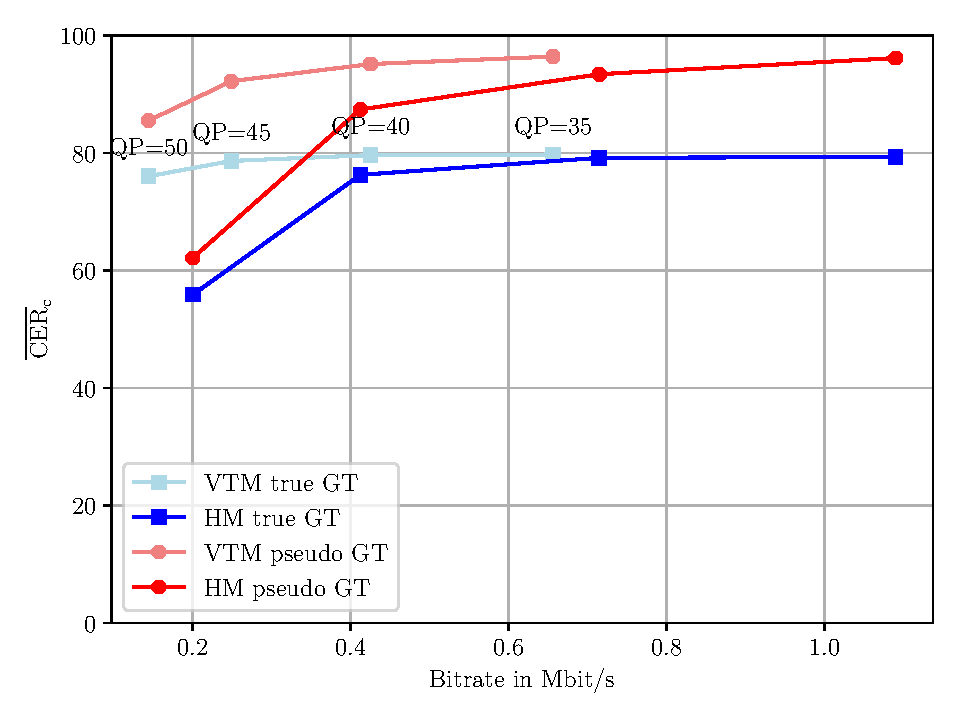
\includegraphics[width=\textwidth]{../images/analyze/codec_cer_size_ezocr_default.pdf}
    \caption{Rate-distortion curves for $\overline{\text{CER}}_{\text{c}}$ vs bitrate for selected images encoded with the HM and VTM codec with the default configuration for EasyOCR.}
    \label{fig:codec_cer_size_ezocr_default}
\end{figure}

In \autoref{fig:codec_cer_size_ezocr_default}, we can see the $\overline{\text{CER}}_{\text{c}}$ in relation to the pseudo and the true \gls{gt} against the size of the images for the HM and VTM codec with the default codec configuration for EasyOCR.
We can observe that the VTM curves are generally further to the top left corner, compared to the HM curves.
This means that the \gls{ocr} algorithm performs better on the VTM encoded images and they are smaller in size.
Additionally, we can see that the trends of the true \gls{gt} curve pair (blue) are similar to the trends of the pseudo \gls{gt} curve pair (red).
To quantify this, we later calculate the \gls{bdrate} between these curves.

\begin{figure}[h!]
    \centering
    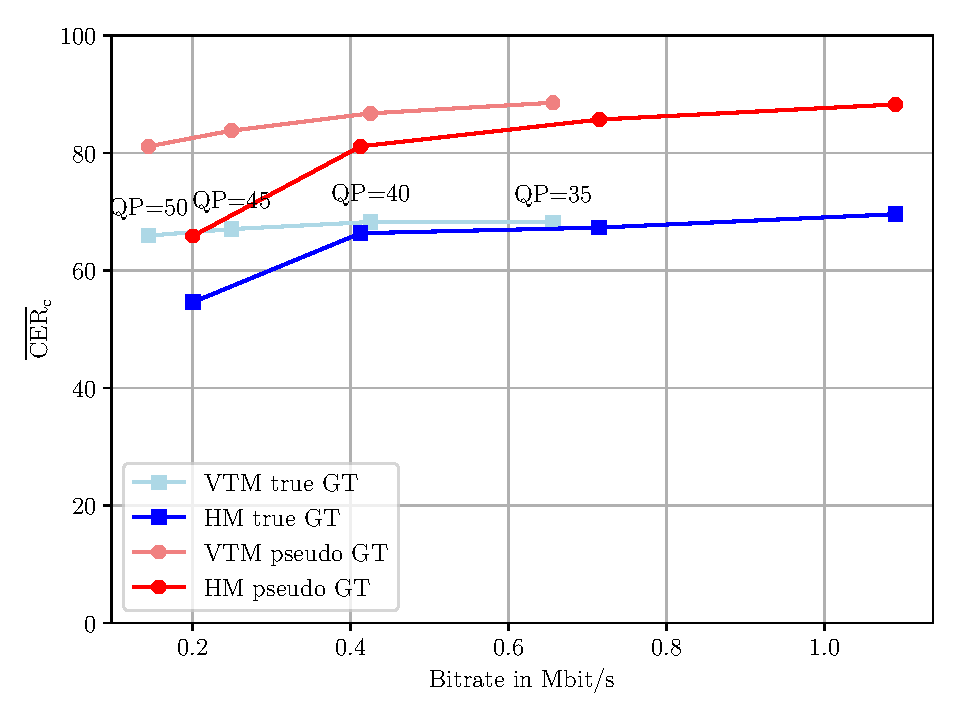
\includegraphics[width=\textwidth]{../images/analyze/codec_cer_size_tess_default.pdf}
    \caption{Rate-distortion curves for $\overline{\text{CER}}_{\text{c}}$ vs bitrate for selected images encoded with the HM and VTM codec with the default configuration for Tesseract \gls{ocr}.}
    \label{fig:codec_cer_size_tess_default}
\end{figure}

In \autoref{fig:codec_cer_size_tess_default}, we can see the same curves with the default codec configuration for Tesseract.
We can again observe that the VTM curves are generally further to top left, compared to the HM curves.
One exception is the \gls{qp} 35, where the VTM codec has a slightly lower $\overline{\text{CER}}_{\text{c}}$ than the HM codec, but still much less bitrate.
When comparing the two blue curves with the two red curves, we can again see the similar trends.
However, for the light blue curve the value for \gls{qp} 35 are lower than for \gls{qp} 40.
In this case we are not able to calculate the \gls{bdrate} between the curves, since one of the curves is not monotonically increasing.


\begin{figure}[h!]
    \centering
    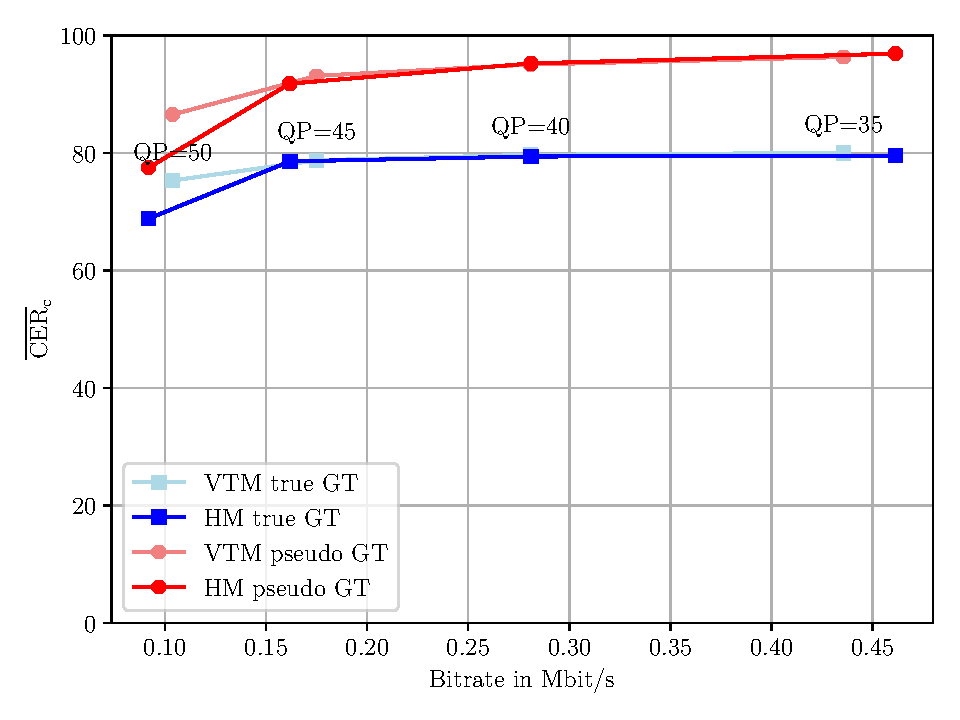
\includegraphics[width=\textwidth]{../images/analyze/codec_cer_size_ezocr_scc.pdf}
    \caption{Rate-distortion curves for $\overline{\text{CER}}_{\text{c}}$ vs bitrate for selected images encoded with the HM and VTM codec with the \gls{scc} configuration for EasyOCR.}
    \label{fig:codec_cer_size_ezocr_scc}
\end{figure}

In \autoref{fig:codec_cer_size_ezocr_scc}, we can see same curves with the \gls{scc} codec configuration for EasyOCR.
The \gls{scc} configuration enables the HM codec to perform similarly to the VTM codec, with the exception of using a \gls{qp} of 50, where the VTM performs better.
When comparing the blue and red curves, we can see that the trends are very similar.


\begin{figure}[h!]
    \centering
    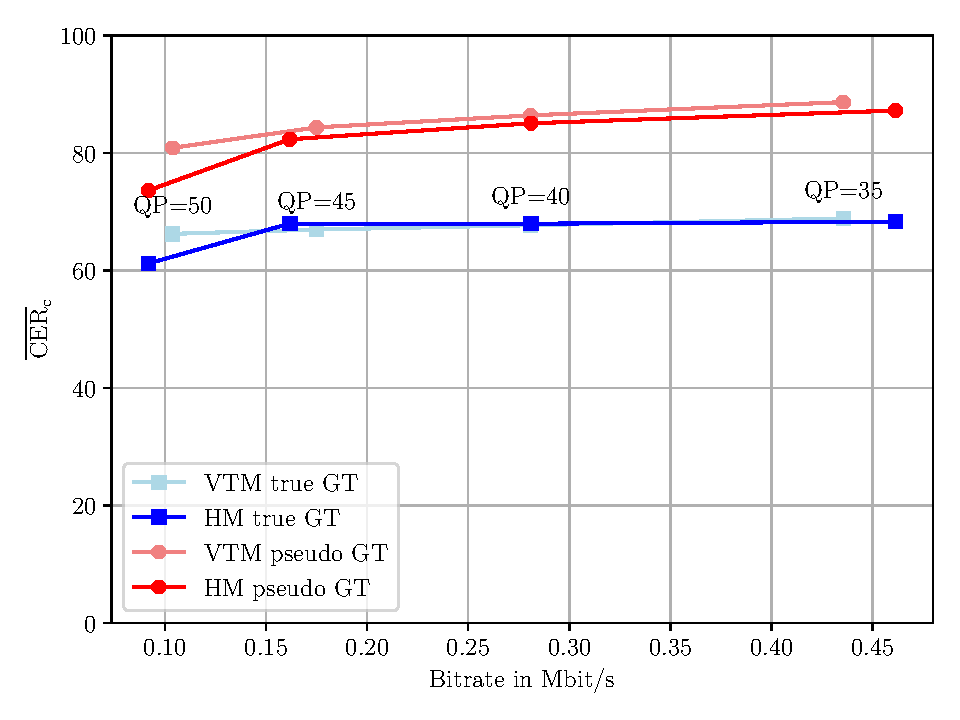
\includegraphics[width=\textwidth]{../images/analyze/codec_cer_size_tess_scc.pdf}
    \caption{Rate-distortion curves for $\overline{\text{CER}}_{\text{c}}$ vs bitrate for selected images encoded with the HM and VTM codec with the \gls{scc} configuration for Tesseract \gls{ocr}.}
    \label{fig:codec_cer_size_tess_scc}
\end{figure}

In \autoref{fig:codec_cer_size_tess_scc}, we can see the same curves with the \gls{scc} codec configuration for Tesseract.
We can see the same phenomenon of the HM codec performing similarly to the VTM codec, with the exception of using a \gls{qp} of 50, where the VTM codec performs better.
When comparing the blue and red curves, we can see that the trends are not similar.
For the true \gls{gt}, the HM codec performs better than the VTM codec, while for the pseudo \gls{gt} the VTM codec performs better than the HM codec.

\begin{table}[h!]
    \centering
    \begin{tabular}{|cc|cc|c|}
        \hline
        % algo, config, pseudo, true, diff
        \gls{ocr} Algorithm & Codec Configuration & Pseudo GT & True GT & Difference \\
        \hline
        \hline
        EasyOCR & Default & -59.28 & -61.02 & 1.73 \\
        EasyOCR & \gls{scc} & -7.41 & -1.1 & -6.32 \\
        \hline
        Tesseract & Default & -54.15 & --- & --- \\
        Tesseract & \gls{scc} & -25.24 & --- & --- \\
        \hline
    \end{tabular}
    \caption{Comparison of $\Delta R$ in \% between the pseudo and the true \gls{gt} for the different \gls{ocr} algorithms and codec configurations.}
    \label{tab:bd_rate}
\end{table}

From \autoref{tab:bd_rate}, we can see that the \gls{bdrate} is way higher for the default configuration than for the \gls{scc} configuration for both the pseudo and the true \gls{gt}.
This reflects the large average distance of the curves seen in \autoref{fig:codec_cer_size_ezocr_default} and \autoref{fig:codec_cer_size_tess_default}, compared to the almost non existent distance seen in \autoref{fig:codec_cer_size_ezocr_scc} and \autoref{fig:codec_cer_size_tess_scc}.
For Tesseract \gls{ocr} we could not calculate the $\Delta R$ for the true \gls{gt}, since the curves are not monotonically increasing.
The difference between the pseudo and the true \gls{gt} is low with $1.73\%$ for the default configuration, but relatively high with $-6.31\%$ for the \gls{scc} configuration.
We can conclude that for images encoded with the default configurations of the HM and VTM codecs, EasyOCR can produce a good pseudo \gls{gt}.

To summarize, we can see that the \gls{ocr} algorithms perform better on the VTM encoded images than on the HM encoded images.
Additionally, the \gls{scc} configuration makes the HM codec perform very similarly to the VTM codec.
It seems like the \gls{scc} configuration manages to keep the text readable even for high \glspl{qp} values.
For the default configuration, EasyOCR seems to be a good pseudo \gls{gt}.
In contrast, Tesseract \gls{ocr} is most likely not suitable for creating a pseudo \gls{gt}, as we were not able to calculate the \gls{bdrate}.
